\documentclass[12pt]{article}
\usepackage[T1]{fontenc}
\usepackage[titletoc]{appendix}
\usepackage[utf8]{inputenc}
\usepackage{CJKutf8}
\usepackage{wrapfig}
\usepackage[font={scriptsize}]{caption}
\usepackage{hyperref}
\usepackage{tikz}
\usepackage{amsmath}



\usetikzlibrary{positioning,shapes,arrows,matrix,calc}

\bibliographystyle{ieeetr}

\newcommand{\brand}{}
\newcommand{\degrees}{\,^{\circ}\mathrm{C}}


\title{\textbf{DORI: Distributed Outdoor \\ Robotic Instruments \\ \large  \textsc{Hardware Design}}}
\author{Andrew Fuller \\ Vedran Budimčić}
\renewcommand{\abstractname}{\large \textsc{Abstract}}
\begin{document}

\pagenumbering{gobble}
\maketitle
\vspace{15mm}
\begin{abstract}
\textsc{DORI} (Distributed Outdoor Robotic Instruments) is a remotely controlled vehicle that is designed to simulate a planetary exploration mission. \textsc{DORI} is equipped with over 20 different environment sensors and can perform basic data analysis, logging and remote upload. The individual components are distributed across a fault-tolerant bus for redundancy. A partial sensor list includes atmospheric pressure, rainfall, wind speed, GPS, gyroscopic inertia, linear acceleration, magnetic field strength, temperature, laser and ultrasonic distance sensing, as well as digital audio and video capture. The project uses recycled consumer electronics devices as a low-cost source for sensor components. This report describes the hardware design of DORI including sensor electronics, embedded firmware, and physical construction.
\end{abstract}
\newpage
\tableofcontents
\newpage
\pagenumbering{arabic}


\section{Introduction}
Few engineering projects require as much careful planning and execution as NASA's space exploration missions. On deployment they are permanently launched to remote locations that make them completely inaccessible to further physical repairs. This thesis describes a planetary exploration mission with self-imposed accessibility and communications constraints, in order to examine a few of the engineering challenges that NASA's mission designers must overcome.



\section{Project Overview}
\subsection{Description}
\textsc{DORI} is a remotely controlled vehicle containing a distributed network of nodes able to remotely measure and record environmental data, which are transmitted to a server for manual analysis. To perform this analysis we have created a suite of data visualization tools called \textsc{tk} that allows us to filter, visualize, and interpret the data recorded by \textsc{DORI}. They present a standard interface for the generation of charts, graphs and plots, as well as the creation of simple 3D reconstructions of the sites where the data were captured. We have also created \textsc{gateway}, a central server to receive and archive the data uploaded by \textsc{DORI}, in addition to performing simple data preprocessing and normalization.

    For the majority of its operating lifetime DORI will simply record the measurements output by the various nodes onto one of two SD cards (referred to as \emph{passive mode}). Once a large batch of sensor values have been collected, one of the uplink nodes will connect to \textsc{gateway} and transfer the full sensor log in a single transfer. A CRC-16 checksum is then computed on both sides and these checksums are compared to confirm that the file was successfully transferred. After a successful transfer the log file can be safely deleted from the logging node.

    In addition to DORI's passive mode of operation, we are also able to send and monitor traffic directly on DORI's system bus using either of the two uplink modems (referred to as \emph{active mode}). TODO add more information here

\subsection{Objectives}
Our aim for this project was to create a fault tolerant distributed data collection system to be deployed to a location that is not easily accessible after launch. DORI will be deployed to a location several hundred kilometers away to guarantee that we were not able to perform any physical repairs after launch. In this way we hope to artificially recreate the risk and uncertainty of a space mission. We intend for \textsc{DORI} to 6remain operational for a minimum of 12 months after deployment. After launch, we plan on conducting simple experiments with all included sensing equipment to record the state of the environment.

For the construction of the device we focused on finding the cheapest possible sources for the required components. The majority of the electronic components in \textsc{DORI} were purchased from retailers in China. Most of the materials used to construct the chassis, ar,m and sensor plate were salvaged from a junkyard at little or no cost. 

The processing power of \textsc{DORI} is distributed among a dozen microcontroller nodes that are each responsible for specific groups of functions. Each node manages a limited number of devices. In this way, the robot is protected from severe malfunction in the event that a single node fails.

Despite being inaccessible after deployment, \textsc{DORI} will inevitably require upgrades and maintenance. Due to this requirement we have included the ability to remotely upgrade the firmware of any node in the distributed system.


\section{System core}
DORI's core is comprised of a collection of nodes distributed over a main system bus. The primary goal in DORI's design was to ensure that the main architecture was highly reliable, with several redundant systems in place to protect against hardware failure. 
developed using atmega88. were short on space for several nodes, so we decided to increase the chip size instead of reducing code size, because that would risk the reliability.

\begin{figure}[h]
    \centering
    \definecolor{cffffff}{RGB}{255,255,255}


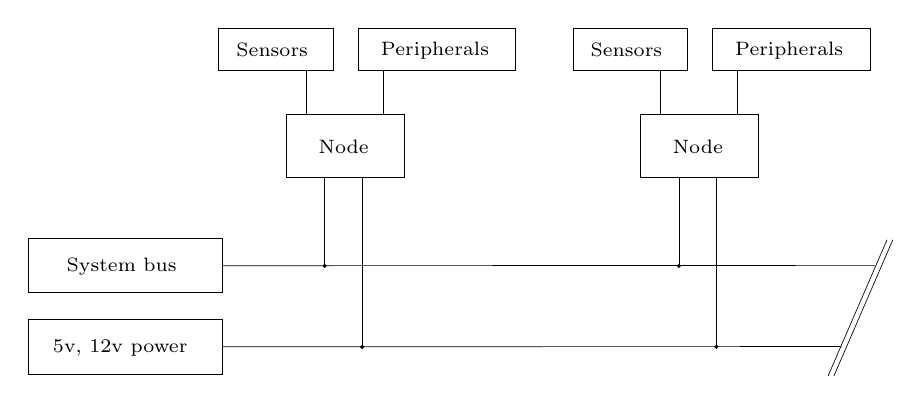
\begin{tikzpicture}[y=0.80pt,x=0.80pt,yscale=-1, inner sep=0pt, outer sep=0pt]
\tikzstyle{every node}=[font=\scriptsize]
\begin{scope}[cm={{1.25,0.0,0.0,-1.25,(0.0,420.0)}}]
  \path[xscale=1.000,yscale=-1.000,draw=black,miter limit=4.38,line
    width=0.240pt,rounded corners=0.0000cm] (41.3070,-168.2285) rectangle
    (111.4056,-148.4549);
  \path[xscale=1.000,yscale=-1.000,fill=black] (55.290295,-154.72006) node[above
    right] (text4399) {System bus};
  \path[xscale=1.000,yscale=-1.000,draw=black,miter limit=4.38,line
    width=0.240pt,rounded corners=0.0000cm] (41.3070,-138.7317) rectangle
    (111.4056,-118.9581);
  \path[xscale=1.000,yscale=-1.000,fill=black] (50.328854,-125.29317) node[above
    right] (text4405) {5v, 12v power};
  \path[draw=black,line join=miter,line cap=butt,miter limit=4.38,line
    width=0.240pt] (111.4056,128.8580) -- (335.1013,128.9552);
  \path[draw=black,line join=miter,line cap=butt,miter limit=4.38,line
    width=0.240pt] (111.4056,158.1552) -- (347.5340,158.2832);
  \begin{scope}[cm={{1.31622,0.0,0.0,1.31682,(1.67945,-77.33039)}},miter limit=4.38,line width=0.240pt]
      \path[xscale=1.000,yscale=-1.000,draw=black,miter limit=4.38,line
        width=0.182pt,rounded corners=0.0000cm] (101.0592,-220.3038) rectangle
        (133.2734,-203.1575);
      \path[xscale=1.000,yscale=-1.000,fill=black] (109.90815,-209.69177) node[above
        right] (text4421) {Node};
      \path[draw=black,line join=miter,line cap=butt,miter limit=4.38,line
        width=0.182pt] (111.5333,203.1575) -- (111.5333,178.7671);
      \path[draw=black,line join=miter,line cap=butt,miter limit=4.38,line
        width=0.182pt] (121.8425,203.1575) -- (121.8425,156.4616);
      \begin{scope}[cm={{1.77172,0.0,0.0,1.77172,(-66.37583,-119.47174)}},miter limit=4.38,line width=0.135pt]
        \path[cm={{0.8,0.0,0.0,-0.8,(0.0,336.0)}},draw=black,fill=black,miter
          limit=4.38,line width=0.129pt] (125.8876,209.5633) .. controls
          (125.8876,209.7678) and (125.7217,209.9337) .. (125.5172,209.9337) .. controls
          (125.3126,209.9337) and (125.1468,209.7678) .. (125.1468,209.5633) .. controls
          (125.1468,209.3587) and (125.3126,209.1929) .. (125.5172,209.1929) .. controls
          (125.7217,209.1929) and (125.8876,209.3587) .. (125.8876,209.5633) -- cycle;
      \end{scope}
      \path[xscale=1.000,yscale=-1.000,draw=black,miter limit=4.38,line
        width=0.182pt,rounded corners=0.0000cm] (82.4284,-244.0851) rectangle
        (113.9330,-232.4201);
      \path[xscale=1.000,yscale=-1.000,fill=black] (87.330894,-236.26181) node[above
        right] (text4446) {Sensors};
      \path[xscale=1.000,yscale=-1.000,fill=black] (127.0157,-235.35158) node[above
        right] (text4450) {Peripherals};
      \path[xscale=1.000,yscale=-1.000,draw=black,miter limit=4.38,line
        width=0.182pt,rounded corners=0.0000cm] (120.8283,-244.0851) rectangle
        (163.9980,-232.4201);
      \path[draw=black,line join=miter,line cap=butt,miter limit=4.38,line
        width=0.182pt] (106.5148,232.5140) -- (106.5148,220.5636);
      \path[draw=black,line join=miter,line cap=butt,miter limit=4.38,line
        width=0.182pt] (127.5580,232.5140) -- (127.5580,220.5636);
      \begin{scope}[cm={{1.77172,0.0,0.0,1.77172,(-56.04266,-141.69955)}},miter limit=4.38,line width=0.135pt]
        \path[cm={{0.8,0.0,0.0,-0.8,(0.0,336.0)}},draw=black,fill=black,miter
          limit=4.38,line width=0.129pt] (125.8876,209.5633) .. controls
          (125.8876,209.7678) and (125.7217,209.9337) .. (125.5172,209.9337) .. controls
          (125.3126,209.9337) and (125.1468,209.7678) .. (125.1468,209.5633) .. controls
          (125.1468,209.3587) and (125.3126,209.1929) .. (125.5172,209.1929) .. controls
          (125.7217,209.1929) and (125.8876,209.3587) .. (125.8876,209.5633) -- cycle;
      \end{scope}
    \begin{scope}[shift={(97.24784,0)}]
      \path[xscale=1.000,yscale=-1.000,draw=black,miter limit=4.38,line
        width=0.182pt,rounded corners=0.0000cm] (101.0592,-220.3038) rectangle
        (133.2734,-203.1575);
      \path[xscale=1.000,yscale=-1.000,fill=black] (109.90815,-209.69177) node[above
        right] (text4845) {Node};
      \path[draw=black,line join=miter,line cap=butt,miter limit=4.38,line
        width=0.182pt] (111.5333,203.1575) -- (111.5333,178.7671);
      \path[draw=black,line join=miter,line cap=butt,miter limit=4.38,line
        width=0.182pt] (121.8425,203.1575) -- (121.8425,156.4616);
      \begin{scope}[cm={{1.77172,0.0,0.0,1.77172,(-66.37583,-119.47174)}},miter limit=4.38,line width=0.135pt]
        \path[cm={{0.8,0.0,0.0,-0.8,(0.0,336.0)}},draw=black,fill=black,miter
          limit=4.38,line width=0.129pt] (125.8876,209.5633) .. controls
          (125.8876,209.7678) and (125.7217,209.9337) .. (125.5172,209.9337) .. controls
          (125.3126,209.9337) and (125.1468,209.7678) .. (125.1468,209.5633) .. controls
          (125.1468,209.3587) and (125.3126,209.1929) .. (125.5172,209.1929) .. controls
          (125.7217,209.1929) and (125.8876,209.3587) .. (125.8876,209.5633) -- cycle;
      \end{scope}
      \path[xscale=1.000,yscale=-1.000,draw=black,miter limit=4.38,line
        width=0.182pt,rounded corners=0.0000cm] (82.4284,-244.0851) rectangle
        (113.9330,-232.4201);
      \path[xscale=1.000,yscale=-1.000,fill=black] (87.330894,-236.26181) node[above
        right] (text4859) {Sensors};
      \path[xscale=1.000,yscale=-1.000,fill=black] (127.0157,-235.35158) node[above
        right] (text4863) {Peripherals};
      \path[xscale=1.000,yscale=-1.000,draw=black,miter limit=4.38,line
        width=0.182pt,rounded corners=0.0000cm] (120.8283,-244.0851) rectangle
        (163.9980,-232.4201);
      \path[draw=black,line join=miter,line cap=butt,miter limit=4.38,line
        width=0.182pt] (106.5148,232.5140) -- (106.5148,220.5636);
      \path[draw=black,line join=miter,line cap=butt,miter limit=4.38,line
        width=0.182pt] (127.5580,232.5140) -- (127.5580,220.5636);
      \begin{scope}[cm={{1.77172,0.0,0.0,1.77172,(-56.04266,-141.69955)}},miter limit=4.38,line width=0.135pt]
        \path[cm={{0.8,0.0,0.0,-0.8,(0.0,336.0)}},draw=black,fill=black,miter
          limit=4.38,line width=0.129pt] (125.8876,209.5633) .. controls
          (125.8876,209.7678) and (125.7217,209.9337) .. (125.5172,209.9337) .. controls
          (125.3126,209.9337) and (125.1468,209.7678) .. (125.1468,209.5633) .. controls
          (125.1468,209.3587) and (125.3126,209.1929) .. (125.5172,209.1929) .. controls
          (125.7217,209.1929) and (125.8876,209.3587) .. (125.8876,209.5633) -- cycle;
      \end{scope}
    \end{scope}
  \end{scope}
  \path[draw=black,line join=miter,line cap=butt,miter limit=4.38,line
    width=0.240pt] (351.7073,167.5268) -- (330.4212,118.3501);
  \path[draw=black,line join=miter,line cap=butt,miter limit=4.38,line
    width=0.240pt] (353.8132,167.5268) -- (332.5272,118.3502);
\end{scope}
\end{tikzpicture}
    \caption{Core system design}
\end{figure}

    \subsection{Message bus}
    DORI's main system backbone is a CAN (Controller Area Network) bus operating at 250kbit/s. 
electrically robust
multi-master
every node has identical interface: atmega88, 
"backbone"

    \subsection{Uplink}
    The uplink connection used by DORI to communicate with our \textsc{gateway} server must always be available to receive new commands and transmit sensor readings. If the uplink were to fail we would be completely unable to read sensor values or dignose the circumstances that caused the failure. We decided to install a minimum of two uplink modems: one for normal use, and another for emergency communications.

    Several communications strategies were evaluated for DORI's main uplink. We first decided to use an RF transceiver, sending Olivia MFSK-encoded AX.25 data over the HF frequency range using hobbyist HAM equipment\cite{olivia-mfsk}. This packet radio format would give us 1200 baud bidirectional transfer at distances of hundreds of kilometers using NVIS (skywave) propagation. We also attempted to design a mechanism where DORI would deploy a 7.5m monopole antenna directly onto the ground to transmit on the 5MHz/60m band. Eventually we decided that this solution had too many drawbacks including weather interference, low transmission range, and high power usage, and was abandoned.

    We finally decided that we would allow ourselves to piggyback off the existing cellular mobile network infrastructure that installed throughout the country in order to simplify the project implementation. Two GSM cellular modems were purchased: a \brand{BenQ m32} USB GSM modem as a main modem, and a \brand{Nokia 3390} cellular phone with SMS capability as a backup modem. These were taken apart and wires were soldered to the respective debugging pins.

    DORI communicates with our \textsc{gateway} server on the cellular network using its main modem, which uses the \brand{7-11 SpeakOut} network at 850/1900MHz. The module's existing antenna was a simple stub of metal, so we replaced its antenna with an external GSM antenna meant for vehicle use, increasing its signal strength by approximately 2dB. The module includes a \brand{Prolific PL2303} USB-serial controller which we have bypassed in order to directly access the \brand{m32} chip's 3.3v UART input and output signals\cite{m32}.

    \subsection{Nodes}
        \subsubsection{AVR}
        Each node consists of an \brand{Atmel AVR ATmega88} microcontroller connected to a number of external sensors and peripherals, with 8192 bytes of Flash program memory and 1024 bytes of RAM. Every node runs a custom event loop configured to the specific peripherals controlled by it, rather than a generic task-switching operating system. Due to the lightweight nature of the driver software and event loop system, most of our node firmware is smaller than 2000 bytes (notable exceptions are the FAT16 driver and the NMEA datestamp parsing code.)

        Node firmware is deliberately simple, and very little pre-processing is performed by DORI. Most drivers are simple wrappers which read sensor values, perform simple low-pass filtering, normalization, and these semi-processed sensor values are directly broadcast on the system bus to be logged and uploaded for analysis. All CPU-intensive processing is performed by \textsc{gateway} or \textsc{tk}. Support circuitry is also minimal, using whatever components are required to interface a particular signal with the AVR.
        
        Nodes are powered by a dual 12v/5v regulated supply. Any node which must interface with peripherals running at voltages other than 5v or 12v has its own power regulator based on the LM2596 step-down (buck) regulator. In particular, nodes interfacing with a large number of 3.3v peripherals have their AVR microcontroller powered by 3.3v, and only the \brand{MCP2515/MCP2551} CAN interface circuitry is powered by 5v.

        \subsubsection{Data reporting}
kalman filter, "filtering sensor data with a kalman filter", interactive-matter.eu
Rolling-average filter, 
\section{Construction}
    \subsection{Chassis}
The main chassis was constructed primarily of salvaged materials. An old streetlight enclosure was used for the frame, a broken floor jack was used as the actuator arm, and the wheels were taken from an old farm tractor. The two chassis components that could not be sourced from a junkyard were the linear actuator used to raise and lower the arm and the stepper motor to rotate the sensor plate. These were bought online from China at low cost.

    \subsection{Drive system}
    DORI uses a simple drive system consisting of two electric motors driving four wheels. The motors are 12v power window motors from a vehicle, with built-in 20:1 gear reduction. The motors are directly connected to the drive shafts, which are lawn mower drive axles giving a further 6:1 gear reduction, for a total gear ratio of 120:1. The wheels on each side of the robot are directly linked together with a chain giving us simulated four-wheel drive using only two motors. This drive configuration is similar to a tank, and having a zero turning radius greatly simplifies our ability to control DORI's position.

    Due to the rough terrain of the target environment we had originally planned to use treads for DORI's drive system, and several designs were considered. Eventually we decided that we did not have enough experience or confidence to attempt to build treads, and the final design uses rubber tractor wheels that are directly connected to the axles.

    \subsection{Actuator arm}
    The actuator arm is built from a car floor jack and is raised and lowered by a 12v linear actuator. When designing the arm structure our priority was to make sure that it was physically secure and would not be affected/influenced by debris or strong winds. The linear actuator has a rated dynamic lifting capacity of 110lbs (50kg), but this capacity is reduced due to the lever configuration of the arm mechanism. During testing we were able to raise a 40kg bag of sand with no noticeable strain on the lifting mechanism. The static holding strength of the linear actuator is 500lbs (226kg) when power is removed, so the arm is unlikely to drift from a raised position when supporting the sensor plate and attached instruments (5kg). During testing we lowered the arm to an almost horizontal position and placed a 40kg bag of sand on top for 12 hours, with no measurable change in height.

    The linear actuator we purchased has an integrated precision linear potentiometer which is able to measure the position of the actuator arm. We are using this as a feedback mechanism to report the arm's position while it's being raised or lowered. The arm's position is also periodically monitored while the arm is static to immediately notify \textsc{tk} of any gradual drift that may occur.

    \subsection{Power}
    DORI is powered by two 12v vehicle batteries each rated to deliver 54Ah. One battery is used to power the electronic components, and the other battery is used to power all of the high-current power electronics. In this configuration they are completely isolated from each other, and the sensors will be protected from electrical noise from the motors. The batteries are constantly recharged by twin 5W solar panels during daylight hours. The electronic circuits draw very little current -- the main system bus and the nodes themselves could run for years on a single charge. The biggest power draw is the various motors, which draw up to 3A when stalled. However DORI has no self-navigation abilities and must be manually controlled, and this will be performed very rarely. The surrounding environment must be studied using \textsc{tk} and a path must be chosen before any drive commands are sent. Therefore DORI will usually stay in a single spot and record measurements. The motors will be used very infrequently so their power draw will be minimal over time.

    \subsection{Nodes}
    Every node is constructed from an identical base circuit layout, with specific hardware modifications added to accomodate the particular peripherals connected to a particular node. The main processor in each node is an Atmel ATmega88 chip clocked from an 8MHz quartz crystal oscillator. Each node connects to the system bus using a Microchip MCP2515 CAN controller connected to a MCP2551 CAN transceiver.

    SCREEN READING TECHNIQUE: fish finders  etc static LCD, 
static lcd, negative voltage, silicon germanium diode clamp to -0.3v.

    wire tap connectors, male spade connectors

The AVR microcontrollers used in DORI have internal RC oscillators that can be used as a cheap low-precision system clock. During testing we found it was possible to achieve communication at low-speed CAN frequencies (below 40kHz) using the RC oscillator within each node's AVR to clock the various peripherals connected to that node. This allowed us to reduce the number of components needed within each bus node. However the RC oscillator's high clock drift was found to interfere with many of the screen signal-sniffing techniques used to connect some display-based peripherals. The affected drivers were rewritten using a technique where the screen is read in several passes, selectively skipping different parts of the signal until a full screen reconstruction is achieved. However we were not able to achieve reliable results using this technique, and it was decided that the convenience of crystal oscillators outweighed the increased component count.

    \subsection{Durability}
We intend to operate \textsc{DORI} for a minimum of 12 months after deployment, so physical reliability is critical. \textsc{DORI} will be operating in a densely forested environment in temperatures ranging from $-6\degrees{}$ to $24\degrees{}$, with an average snowfall of over 400cm.

Other possible hazards include rats, water condensation, and electrical interference due to thunderstorms. Rats love to chew wires, so we have insulated all exposed wires with armored cable for protection. Most of the signals within \textsc{DORI} are relatively low frequency, so they will not be very susceptible to EM interference. We wanted to avoid any kind of condensation inside the enclosed electronic circuits, so each moisture-sensitive module underwent a waterproofing procedure. We first placed dessicant packets from ramen noodles into any large enclosed spaces, and then used a home hair dryer to heat and dry the air that would remain sealed with the electronics. Once the air was sufficiently dry we used a rubberized chemical spray to completely coat the electrical components in a water-tight rubber barrier.


\section{Peripherals}
\subsection{Sensors}
\subsubsection{Atmospheric}
The primary mission objective is to record remote environmental measurements and transfer the data back to \textsc{tk} to be manually analyzed. The sensors which record atmospheric conditions are therefore very critical to help us study the environment of the target site.
    \paragraph*{Temperature}
    The temperature sensor that we decided to use was the \brand{Maxim DS18B20} 1-Wire Digital Temperature Sensor, due to the authors' prior experience with this particular device. These sensors have a measurement range of $-55\degrees{}$ to $+125\degrees{}$, with $\pm0.5\degrees{}$ accuracy from $-10\degrees{}$ to $+85\degrees{}$. They are pre-calibrated and can be connected using a single wire simultaneously carrying data and power. These were acquired as free samples from Maxim Semiconductor, and are installed among the various components to rather external as well as internal temperature readings.

    Maxim's 1-Wire devices are able to be individually addressed over a shared data wire, referred to as a 1-Wire network. The 1-Wire search algorithm is conceptually similar to the bus arbitration used by CAN. Individual bits are queried across each possible device identifier, and any matching devices are further specified until they can be uniquely identified by the bits that have been included in the query\cite{1wiresearch}. Using this search algorithm, we can place hundreds of 1-Wire sensors across the robot, all interfaced via a single system bus node. For our purposes we decided to include 12 temperature sensors placed inside and outside the robot frame, as well as scattered among the heat-sensitive electronic components, and one temperature sensor for each of the four motors (stepper motor, linear actuator, and both drive motors.)

    \paragraph*{Air pressure}
    We picked the \brand{Bosch BMP085} barometric pressure sensor primarily due to the number of inexpensive hobbyist-level development modules available from online suppliers. This is an \textsc{i2c} sensor which outputs a raw pressure value from a sensing element. A compensation algorithm is also provided which is used to convert the raw sensor values to calibrated barometric pressure measurements. The output from this sensor is subject to various sources of noise (such as changing weather patterns) and is not directly useful as an environmental measurement. However when this value is averaged over several days it can be used as a high-resolution altimeter. The current barometric pressure reading can thus be compared to the average pressure for a particular altitude to provide meteorological measurements about incoming storms or other pressure systems.

    \paragraph*{Wind velocity}
There are many common wind speed and direction sensor designs, most of which use a rotating wheel anemometer to measure wind speed combined with a wind vane to measure wind direction. These designs are delicate and difficult to seal against moisture and debris. There are also cheap handheld digital units such as the \textsc{GM8908}\cite{gm8908} for \$14, but most of these are unidirectional.

There is a new design that has become increasingly popular due to its small size and solid-state nature. A small current is drawn through a thin piece of wire until it reaches a certain temperature. Air moving past the wire cools it down, and increases the current needed to maintain a steady temperature. This current maintains an approximately linear relationship with the wind speed. However the sensor element itself is fragile and care must be taken to avoid direct exposure to moisture.

Another important aspect of the wind sensor is that our storage space is very limited, so DORI will likely be limited to a few wind measurements each hour. We will also likely never need an instantaneous wind velocity measurement. This means that we can use a simpler sensor that may produce large amounts of noise, and then average the output to create more accurate \emph{average} wind velocity measurements.

We decided to use a radically simpler design with fewer moving parts, while sacrificing linear response and output accuracy. We attached a Wii Nunchuck containing an Analog Devices \textsc{ADXL335} accelerometer to the end of a flexible plastic tube mounted vertically to the robot's body. The tube is further wrapped in thick foam to increase its wind resistance. As the tube gets pushed by the wind, the deflection can be measured by the accelerometer mounted at the top. This means that the entire device can be environmentally sealed with minimal mechanical impact. However this simple design means the sensor's output is highly nonlinear and must be calibrated against several known values before useful wind speed measurements can be recorded. Therefore, we have taken several sample readings using a large electric fan, and calibrated them against simultaneous values from a \textsc{GM8908} unit. We must also compensate for the effect of gravity by subtracting the current tilt of the robot from the wind sensor accelerometer's values.

This wind sensor design can be modelled as a beam with a uniformly distributed load, and the deflection can be calculated as $\Delta x = \frac{wL^4}{8EI}$ where $w$ is the surface stress in $N/m$ created by the wind, $L$ is the length of the beam in $m$, and $EI$ is its flexural stiffness, the product of the Young's modulus of the beam material with its second moment of area, in $Nm^2$. The wind speed is quadratic with respect to the air pressure, so we can expect it to be quadratic with respect to the tube deflection $\Delta x$.

{
    \scriptsize
    % GNUPLOT: LaTeX picture
\setlength{\unitlength}{0.240900pt}
\ifx\plotpoint\undefined\newsavebox{\plotpoint}\fi
\sbox{\plotpoint}{\rule[-0.200pt]{0.400pt}{0.400pt}}%
\begin{picture}(1500,900)(0,0)
\sbox{\plotpoint}{\rule[-0.200pt]{0.400pt}{0.400pt}}%
\multiput(294.00,233.92)(30.709,-0.493){23}{\rule{23.946pt}{0.119pt}}
\multiput(294.00,234.17)(725.299,-13.000){2}{\rule{11.973pt}{0.400pt}}
\multiput(1202.43,292.92)(-0.953,-0.499){141}{\rule{0.861pt}{0.120pt}}
\multiput(1204.21,293.17)(-135.213,-72.000){2}{\rule{0.431pt}{0.400pt}}
\put(294.0,235.0){\rule[-0.200pt]{0.400pt}{99.010pt}}
\put(254,372){\makebox(0,0)[r]{ 510}}
\put(294.0,372.0){\rule[-0.200pt]{4.818pt}{0.400pt}}
\put(254,412){\makebox(0,0)[r]{ 520}}
\put(294.0,412.0){\rule[-0.200pt]{4.818pt}{0.400pt}}
\put(254,451){\makebox(0,0)[r]{ 530}}
\put(294.0,451.0){\rule[-0.200pt]{4.818pt}{0.400pt}}
\put(254,489){\makebox(0,0)[r]{ 540}}
\put(294.0,489.0){\rule[-0.200pt]{4.818pt}{0.400pt}}
\put(254,528){\makebox(0,0)[r]{ 550}}
\put(294.0,528.0){\rule[-0.200pt]{4.818pt}{0.400pt}}
\put(254,568){\makebox(0,0)[r]{ 560}}
\put(294.0,568.0){\rule[-0.200pt]{4.818pt}{0.400pt}}
\put(254,607){\makebox(0,0)[r]{ 570}}
\put(294.0,607.0){\rule[-0.200pt]{4.818pt}{0.400pt}}
\put(254,646){\makebox(0,0)[r]{ 580}}
\put(294.0,646.0){\rule[-0.200pt]{4.818pt}{0.400pt}}
\put(1066,836){\makebox(0,0)[r]{Vertical}}
%\put(1066,756){\makebox(0,0)[r]{Vertical}}
\put(1136,836){\makebox(0,0){$+$}}
\put(417,404){\makebox(0,0){$+$}}
\put(417,404){\makebox(0,0){$+$}}
\put(443,424){\makebox(0,0){$+$}}
\put(443,424){\makebox(0,0){$+$}}
\put(443,404){\makebox(0,0){$+$}}
\put(521,413){\makebox(0,0){$+$}}
\put(521,413){\makebox(0,0){$+$}}
\put(475,403){\makebox(0,0){$+$}}
\put(501,423){\makebox(0,0){$+$}}
\put(475,443){\makebox(0,0){$+$}}
\put(443,443){\makebox(0,0){$+$}}
\put(443,443){\makebox(0,0){$+$}}
\put(456,413){\makebox(0,0){$+$}}
\put(423,394){\makebox(0,0){$+$}}
\put(385,405){\makebox(0,0){$+$}}
\put(417,424){\makebox(0,0){$+$}}
\put(475,443){\makebox(0,0){$+$}}
\put(443,443){\makebox(0,0){$+$}}
\put(385,444){\makebox(0,0){$+$}}
\put(417,444){\makebox(0,0){$+$}}
\put(475,443){\makebox(0,0){$+$}}
\put(475,443){\makebox(0,0){$+$}}
\put(443,443){\makebox(0,0){$+$}}
\put(475,443){\makebox(0,0){$+$}}
\put(475,443){\makebox(0,0){$+$}}
\put(495,453){\makebox(0,0){$+$}}
\put(463,453){\makebox(0,0){$+$}}
\put(417,444){\makebox(0,0){$+$}}
\put(443,443){\makebox(0,0){$+$}}
\put(443,443){\makebox(0,0){$+$}}
\put(417,444){\makebox(0,0){$+$}}
\put(443,424){\makebox(0,0){$+$}}
\put(443,404){\makebox(0,0){$+$}}
\put(417,404){\makebox(0,0){$+$}}
\put(443,404){\makebox(0,0){$+$}}
\put(443,424){\makebox(0,0){$+$}}
\put(443,443){\makebox(0,0){$+$}}
\put(417,444){\makebox(0,0){$+$}}
\put(463,453){\makebox(0,0){$+$}}
\put(514,463){\makebox(0,0){$+$}}
\put(514,463){\makebox(0,0){$+$}}
\put(514,444){\makebox(0,0){$+$}}
\put(482,444){\makebox(0,0){$+$}}
\put(482,464){\makebox(0,0){$+$}}
\put(495,453){\makebox(0,0){$+$}}
\put(475,443){\makebox(0,0){$+$}}
\put(443,443){\makebox(0,0){$+$}}
\put(443,443){\makebox(0,0){$+$}}
\put(463,453){\makebox(0,0){$+$}}
\put(456,464){\makebox(0,0){$+$}}
\put(437,454){\makebox(0,0){$+$}}
\put(463,453){\makebox(0,0){$+$}}
\put(482,464){\makebox(0,0){$+$}}
\put(514,463){\makebox(0,0){$+$}}
\put(514,463){\makebox(0,0){$+$}}
\put(482,464){\makebox(0,0){$+$}}
\put(482,444){\makebox(0,0){$+$}}
\put(482,424){\makebox(0,0){$+$}}
\put(482,424){\makebox(0,0){$+$}}
\put(482,424){\makebox(0,0){$+$}}
\put(482,424){\makebox(0,0){$+$}}
\put(482,444){\makebox(0,0){$+$}}
\put(463,453){\makebox(0,0){$+$}}
\put(475,443){\makebox(0,0){$+$}}
\put(475,443){\makebox(0,0){$+$}}
\put(443,443){\makebox(0,0){$+$}}
\put(501,442){\makebox(0,0){$+$}}
\put(501,442){\makebox(0,0){$+$}}
\put(417,444){\makebox(0,0){$+$}}
\put(417,444){\makebox(0,0){$+$}}
\put(475,443){\makebox(0,0){$+$}}
\put(475,443){\makebox(0,0){$+$}}
\put(437,454){\makebox(0,0){$+$}}
\put(424,445){\makebox(0,0){$+$}}
\put(482,424){\makebox(0,0){$+$}}
\put(521,433){\makebox(0,0){$+$}}
\put(475,443){\makebox(0,0){$+$}}
\put(443,443){\makebox(0,0){$+$}}
\put(475,443){\makebox(0,0){$+$}}
\put(475,443){\makebox(0,0){$+$}}
\put(437,434){\makebox(0,0){$+$}}
\put(456,425){\makebox(0,0){$+$}}
\put(514,424){\makebox(0,0){$+$}}
\put(514,424){\makebox(0,0){$+$}}
\put(456,425){\makebox(0,0){$+$}}
\put(482,424){\makebox(0,0){$+$}}
\put(514,424){\makebox(0,0){$+$}}
\put(482,444){\makebox(0,0){$+$}}
\put(482,464){\makebox(0,0){$+$}}
\put(463,453){\makebox(0,0){$+$}}
\put(475,443){\makebox(0,0){$+$}}
\put(1066,785){\makebox(0,0)[r]{Light wind}}
%\put(1066,715){\makebox(0,0)[r]{Light wind}}
\put(1136,785){\makebox(0,0){$\times$}}
\put(843,628){\makebox(0,0){$\times$}}
\put(798,595){\makebox(0,0){$\times$}}
\put(856,574){\makebox(0,0){$\times$}}
\put(798,595){\makebox(0,0){$\times$}}
\put(741,596){\makebox(0,0){$\times$}}
\put(766,596){\makebox(0,0){$\times$}}
\put(798,595){\makebox(0,0){$\times$}}
\put(824,575){\makebox(0,0){$\times$}}
\put(824,575){\makebox(0,0){$\times$}}
\put(824,575){\makebox(0,0){$\times$}}
\put(824,595){\makebox(0,0){$\times$}}
\put(798,619){\makebox(0,0){$\times$}}
\put(824,618){\makebox(0,0){$\times$}}
\put(856,618){\makebox(0,0){$\times$}}
\put(817,629){\makebox(0,0){$\times$}}
\put(805,640){\makebox(0,0){$\times$}}
\put(843,628){\makebox(0,0){$\times$}}
\put(824,618){\makebox(0,0){$\times$}}
\put(798,619){\makebox(0,0){$\times$}}
\put(824,595){\makebox(0,0){$\times$}}
\put(824,575){\makebox(0,0){$\times$}}
\put(798,575){\makebox(0,0){$\times$}}
\put(766,596){\makebox(0,0){$\times$}}
\put(798,619){\makebox(0,0){$\times$}}
\put(804,608){\makebox(0,0){$\times$}}
\put(778,608){\makebox(0,0){$\times$}}
\put(798,619){\makebox(0,0){$\times$}}
\put(798,619){\makebox(0,0){$\times$}}
\put(798,619){\makebox(0,0){$\times$}}
\put(798,619){\makebox(0,0){$\times$}}
\put(798,595){\makebox(0,0){$\times$}}
\put(824,575){\makebox(0,0){$\times$}}
\put(798,595){\makebox(0,0){$\times$}}
\put(766,619){\makebox(0,0){$\times$}}
\put(785,629){\makebox(0,0){$\times$}}
\put(863,639){\makebox(0,0){$\times$}}
\put(843,628){\makebox(0,0){$\times$}}
\put(798,619){\makebox(0,0){$\times$}}
\put(798,595){\makebox(0,0){$\times$}}
\put(798,575){\makebox(0,0){$\times$}}
\put(824,575){\makebox(0,0){$\times$}}
\put(798,575){\makebox(0,0){$\times$}}
\put(766,576){\makebox(0,0){$\times$}}
\put(798,575){\makebox(0,0){$\times$}}
\put(766,576){\makebox(0,0){$\times$}}
\put(766,596){\makebox(0,0){$\times$}}
\put(798,595){\makebox(0,0){$\times$}}
\put(798,575){\makebox(0,0){$\times$}}
\put(843,585){\makebox(0,0){$\times$}}
\put(863,595){\makebox(0,0){$\times$}}
\put(817,586){\makebox(0,0){$\times$}}
\put(798,595){\makebox(0,0){$\times$}}
\put(824,618){\makebox(0,0){$\times$}}
\put(798,619){\makebox(0,0){$\times$}}
\put(766,619){\makebox(0,0){$\times$}}
\put(766,596){\makebox(0,0){$\times$}}
\put(766,576){\makebox(0,0){$\times$}}
\put(824,575){\makebox(0,0){$\times$}}
\put(824,575){\makebox(0,0){$\times$}}
\put(766,596){\makebox(0,0){$\times$}}
\put(824,618){\makebox(0,0){$\times$}}
\put(856,618){\makebox(0,0){$\times$}}
\put(798,619){\makebox(0,0){$\times$}}
\put(798,595){\makebox(0,0){$\times$}}
\put(785,586){\makebox(0,0){$\times$}}
\put(805,616){\makebox(0,0){$\times$}}
\put(817,605){\makebox(0,0){$\times$}}
\put(766,576){\makebox(0,0){$\times$}}
\put(798,595){\makebox(0,0){$\times$}}
\put(824,595){\makebox(0,0){$\times$}}
\put(843,605){\makebox(0,0){$\times$}}
\put(837,639){\makebox(0,0){$\times$}}
\put(817,605){\makebox(0,0){$\times$}}
\put(824,575){\makebox(0,0){$\times$}}
\put(798,575){\makebox(0,0){$\times$}}
\put(798,575){\makebox(0,0){$\times$}}
\put(798,575){\makebox(0,0){$\times$}}
\put(798,595){\makebox(0,0){$\times$}}
\put(798,619){\makebox(0,0){$\times$}}
\put(798,619){\makebox(0,0){$\times$}}
\put(824,618){\makebox(0,0){$\times$}}
\put(824,595){\makebox(0,0){$\times$}}
\put(824,575){\makebox(0,0){$\times$}}
\put(766,576){\makebox(0,0){$\times$}}
\put(766,596){\makebox(0,0){$\times$}}
\put(824,595){\makebox(0,0){$\times$}}
\put(824,575){\makebox(0,0){$\times$}}
\put(798,575){\makebox(0,0){$\times$}}
\put(778,565){\makebox(0,0){$\times$}}
\put(785,555){\makebox(0,0){$\times$}}
\put(759,555){\makebox(0,0){$\times$}}
\put(785,555){\makebox(0,0){$\times$}}
\put(837,584){\makebox(0,0){$\times$}}
\put(824,618){\makebox(0,0){$\times$}}
\put(856,618){\makebox(0,0){$\times$}}
\put(824,618){\makebox(0,0){$\times$}}
\put(766,619){\makebox(0,0){$\times$}}
\put(798,595){\makebox(0,0){$\times$}}
\put(766,596){\makebox(0,0){$\times$}}
\put(741,596){\makebox(0,0){$\times$}}
\put(741,576){\makebox(0,0){$\times$}}
\put(766,596){\makebox(0,0){$\times$}}
\put(824,595){\makebox(0,0){$\times$}}
\put(824,595){\makebox(0,0){$\times$}}
\put(798,619){\makebox(0,0){$\times$}}
\put(798,619){\makebox(0,0){$\times$}}
\put(798,619){\makebox(0,0){$\times$}}
\put(766,596){\makebox(0,0){$\times$}}
\put(766,576){\makebox(0,0){$\times$}}
\put(798,575){\makebox(0,0){$\times$}}
\put(824,575){\makebox(0,0){$\times$}}
\put(798,595){\makebox(0,0){$\times$}}
\put(798,595){\makebox(0,0){$\times$}}
\put(798,575){\makebox(0,0){$\times$}}
\put(766,596){\makebox(0,0){$\times$}}
\put(798,595){\makebox(0,0){$\times$}}
\put(798,595){\makebox(0,0){$\times$}}
\put(798,619){\makebox(0,0){$\times$}}
\put(824,595){\makebox(0,0){$\times$}}
\put(798,575){\makebox(0,0){$\times$}}
\put(798,575){\makebox(0,0){$\times$}}
\put(843,585){\makebox(0,0){$\times$}}
\put(843,585){\makebox(0,0){$\times$}}
\put(817,586){\makebox(0,0){$\times$}}
\put(805,596){\makebox(0,0){$\times$}}
\put(817,586){\makebox(0,0){$\times$}}
\put(824,575){\makebox(0,0){$\times$}}
\put(843,585){\makebox(0,0){$\times$}}
\put(843,605){\makebox(0,0){$\times$}}
\put(798,619){\makebox(0,0){$\times$}}
\put(798,619){\makebox(0,0){$\times$}}
\put(824,618){\makebox(0,0){$\times$}}
\put(798,619){\makebox(0,0){$\times$}}
\put(766,619){\makebox(0,0){$\times$}}
\put(766,619){\makebox(0,0){$\times$}}
\put(798,595){\makebox(0,0){$\times$}}
\put(824,575){\makebox(0,0){$\times$}}
%\put(1066,674){\makebox(0,0)[r]{Strong wind}}
\put(1066,734){\makebox(0,0)[r]{Strong wind}}
\sbox{\plotpoint}{\rule[-0.400pt]{0.800pt}{0.800pt}}%
\put(1136,734){\makebox(0,0){$\ast$}}
\put(1070,655){\makebox(0,0){$\ast$}}
\put(1037,675){\makebox(0,0){$\ast$}}
\put(1037,675){\makebox(0,0){$\ast$}}
\put(1037,675){\makebox(0,0){$\ast$}}
\put(1057,685){\makebox(0,0){$\ast$}}
\put(1077,696){\makebox(0,0){$\ast$}}
\put(1051,696){\makebox(0,0){$\ast$}}
\put(999,686){\makebox(0,0){$\ast$}}
\put(1012,676){\makebox(0,0){$\ast$}}
\put(979,656){\makebox(0,0){$\ast$}}
\put(979,637){\makebox(0,0){$\ast$}}
\put(1012,636){\makebox(0,0){$\ast$}}
\put(1012,636){\makebox(0,0){$\ast$}}
\put(1012,636){\makebox(0,0){$\ast$}}
\put(979,637){\makebox(0,0){$\ast$}}
\put(1012,656){\makebox(0,0){$\ast$}}
\put(1057,666){\makebox(0,0){$\ast$}}
\put(1077,676){\makebox(0,0){$\ast$}}
\put(1031,686){\makebox(0,0){$\ast$}}
\put(979,676){\makebox(0,0){$\ast$}}
\put(992,665){\makebox(0,0){$\ast$}}
\put(1018,665){\makebox(0,0){$\ast$}}
\put(992,665){\makebox(0,0){$\ast$}}
\put(960,646){\makebox(0,0){$\ast$}}
\put(1012,636){\makebox(0,0){$\ast$}}
\put(1037,636){\makebox(0,0){$\ast$}}
\put(1037,636){\makebox(0,0){$\ast$}}
\put(1037,656){\makebox(0,0){$\ast$}}
\put(1070,675){\makebox(0,0){$\ast$}}
\put(1037,675){\makebox(0,0){$\ast$}}
\put(953,677){\makebox(0,0){$\ast$}}
\put(953,677){\makebox(0,0){$\ast$}}
\put(1012,676){\makebox(0,0){$\ast$}}
\put(1037,675){\makebox(0,0){$\ast$}}
\put(1037,675){\makebox(0,0){$\ast$}}
\put(1037,656){\makebox(0,0){$\ast$}}
\put(1031,666){\makebox(0,0){$\ast$}}
\put(1031,666){\makebox(0,0){$\ast$}}
\put(1096,655){\makebox(0,0){$\ast$}}
\put(1122,674){\makebox(0,0){$\ast$}}
\put(1037,675){\makebox(0,0){$\ast$}}
\put(979,676){\makebox(0,0){$\ast$}}
\put(1037,656){\makebox(0,0){$\ast$}}
\put(1096,635){\makebox(0,0){$\ast$}}
\put(1089,646){\makebox(0,0){$\ast$}}
\put(1051,676){\makebox(0,0){$\ast$}}
\put(1051,696){\makebox(0,0){$\ast$}}
\put(1051,696){\makebox(0,0){$\ast$}}
\put(1018,697){\makebox(0,0){$\ast$}}
\put(1077,696){\makebox(0,0){$\ast$}}
\put(1109,695){\makebox(0,0){$\ast$}}
\put(1077,676){\makebox(0,0){$\ast$}}
\put(999,647){\makebox(0,0){$\ast$}}
\put(953,657){\makebox(0,0){$\ast$}}
\put(999,686){\makebox(0,0){$\ast$}}
\put(1018,697){\makebox(0,0){$\ast$}}
\put(1051,676){\makebox(0,0){$\ast$}}
\put(1051,657){\makebox(0,0){$\ast$}}
\put(1031,647){\makebox(0,0){$\ast$}}
\put(1012,636){\makebox(0,0){$\ast$}}
\put(1037,636){\makebox(0,0){$\ast$}}
\put(1037,636){\makebox(0,0){$\ast$}}
\put(979,637){\makebox(0,0){$\ast$}}
\put(1012,636){\makebox(0,0){$\ast$}}
\put(979,637){\makebox(0,0){$\ast$}}
\put(999,647){\makebox(0,0){$\ast$}}
\put(1057,646){\makebox(0,0){$\ast$}}
\put(1057,646){\makebox(0,0){$\ast$}}
\put(1031,647){\makebox(0,0){$\ast$}}
\put(1012,636){\makebox(0,0){$\ast$}}
\put(999,647){\makebox(0,0){$\ast$}}
\put(993,658){\makebox(0,0){$\ast$}}
\put(1018,657){\makebox(0,0){$\ast$}}
\put(1018,657){\makebox(0,0){$\ast$}}
\put(1031,647){\makebox(0,0){$\ast$}}
\put(1037,656){\makebox(0,0){$\ast$}}
\put(1037,675){\makebox(0,0){$\ast$}}
\put(1037,656){\makebox(0,0){$\ast$}}
\put(1012,636){\makebox(0,0){$\ast$}}
\put(1012,636){\makebox(0,0){$\ast$}}
\put(1037,636){\makebox(0,0){$\ast$}}
\put(1018,645){\makebox(0,0){$\ast$}}
\put(1031,654){\makebox(0,0){$\ast$}}
\put(998,655){\makebox(0,0){$\ast$}}
\put(973,655){\makebox(0,0){$\ast$}}
\put(992,665){\makebox(0,0){$\ast$}}
\put(979,676){\makebox(0,0){$\ast$}}
\put(1037,675){\makebox(0,0){$\ast$}}
\put(1057,685){\makebox(0,0){$\ast$}}
\put(1031,686){\makebox(0,0){$\ast$}}
\put(1070,675){\makebox(0,0){$\ast$}}
\sbox{\plotpoint}{\rule[-0.200pt]{0.400pt}{0.400pt}}%
\multiput(1098.35,294.58)(-33.367,0.492){21}{\rule{25.933pt}{0.119pt}}
\multiput(1152.17,293.17)(-721.174,12.000){2}{\rule{12.967pt}{0.400pt}}
\multiput(294.00,235.58)(0.967,0.499){139}{\rule{0.872pt}{0.120pt}}
\multiput(294.00,234.17)(135.190,71.000){2}{\rule{0.436pt}{0.400pt}}
\multiput(1069.00,222.61)(1.355,0.447){3}{\rule{1.033pt}{0.108pt}}
\multiput(1069.00,221.17)(4.855,3.000){2}{\rule{0.517pt}{0.400pt}}
%\put(1063,215){\makebox(0,0){ 400}}
\multiput(1202.68,292.94)(-0.920,-0.468){5}{\rule{0.800pt}{0.113pt}}
\multiput(1204.34,293.17)(-5.340,-4.000){2}{\rule{0.400pt}{0.400pt}}
\multiput(940.00,224.60)(0.774,0.468){5}{\rule{0.700pt}{0.113pt}}
\multiput(940.00,223.17)(4.547,4.000){2}{\rule{0.350pt}{0.400pt}}
\put(933,217){\makebox(0,0){ 420}}
\multiput(1073.68,294.94)(-0.920,-0.468){5}{\rule{0.800pt}{0.113pt}}
\multiput(1075.34,295.17)(-5.340,-4.000){2}{\rule{0.400pt}{0.400pt}}
\multiput(810.00,226.60)(0.920,0.468){5}{\rule{0.800pt}{0.113pt}}
\multiput(810.00,225.17)(5.340,4.000){2}{\rule{0.400pt}{0.400pt}}
\put(804,219){\makebox(0,0){ 440}}
\multiput(944.09,296.94)(-0.774,-0.468){5}{\rule{0.700pt}{0.113pt}}
\multiput(945.55,297.17)(-4.547,-4.000){2}{\rule{0.350pt}{0.400pt}}
\multiput(682.00,228.60)(0.920,0.468){5}{\rule{0.800pt}{0.113pt}}
\multiput(682.00,227.17)(5.340,4.000){2}{\rule{0.400pt}{0.400pt}}
\put(676,221){\makebox(0,0){ 460}}
\multiput(813.71,298.95)(-1.355,-0.447){3}{\rule{1.033pt}{0.108pt}}
\multiput(815.86,299.17)(-4.855,-3.000){2}{\rule{0.517pt}{0.400pt}}
\multiput(553.00,230.60)(0.774,0.468){5}{\rule{0.700pt}{0.113pt}}
\multiput(553.00,229.17)(4.547,4.000){2}{\rule{0.350pt}{0.400pt}}
\put(546,223){\makebox(0,0){ 480}}
\multiput(685.71,300.95)(-1.355,-0.447){3}{\rule{1.033pt}{0.108pt}}
\multiput(687.86,301.17)(-4.855,-3.000){2}{\rule{0.517pt}{0.400pt}}
\multiput(423.00,233.61)(1.355,0.447){3}{\rule{1.033pt}{0.108pt}}
\multiput(423.00,232.17)(4.855,3.000){2}{\rule{0.517pt}{0.400pt}}
\put(417,226){\makebox(0,0){ 500}}
\multiput(556.26,302.95)(-1.132,-0.447){3}{\rule{0.900pt}{0.108pt}}
\multiput(558.13,303.17)(-4.132,-3.000){2}{\rule{0.450pt}{0.400pt}}
\multiput(294.00,235.61)(1.355,0.447){3}{\rule{1.033pt}{0.108pt}}
\multiput(294.00,234.17)(4.855,3.000){2}{\rule{0.517pt}{0.400pt}}
\put(288,228){\makebox(0,0){ 520}}
\multiput(426.71,304.95)(-1.355,-0.447){3}{\rule{1.033pt}{0.108pt}}
\multiput(428.86,305.17)(-4.855,-3.000){2}{\rule{0.517pt}{0.400pt}}
\put(1089,221){\makebox(0,0)[l]{ 270}}
\put(1049.0,222.0){\rule[-0.200pt]{4.818pt}{0.400pt}}
\put(294,233.67){\rule{4.818pt}{0.400pt}}
\multiput(294.00,234.17)(10.000,-1.000){2}{\rule{2.409pt}{0.400pt}}
\put(1069,231.67){\rule{4.818pt}{0.400pt}}
\multiput(1079.00,231.17)(-10.000,1.000){2}{\rule{2.409pt}{0.400pt}}
%\put(1108,232){\makebox(0,0)[l]{ 275}}
\put(314.0,245.0){\rule[-0.200pt]{4.577pt}{0.400pt}}
%\put(1128,242){\makebox(0,0)[l]{ 280}}
\put(1088.0,243.0){\rule[-0.200pt]{4.818pt}{0.400pt}}
\put(333.0,255.0){\rule[-0.200pt]{4.818pt}{0.400pt}}
\put(1147,252){\makebox(0,0)[l]{ 285}}
\put(1108.0,253.0){\rule[-0.200pt]{4.818pt}{0.400pt}}
\put(353.0,265.0){\rule[-0.200pt]{4.577pt}{0.400pt}}
%\put(1167,262){\makebox(0,0)[l]{ 290}}
\put(1128.0,263.0){\rule[-0.200pt]{4.577pt}{0.400pt}}
\put(372,274.67){\rule{4.818pt}{0.400pt}}
\multiput(372.00,275.17)(10.000,-1.000){2}{\rule{2.409pt}{0.400pt}}
\put(1147,272.67){\rule{4.818pt}{0.400pt}}
\multiput(1157.00,272.17)(-10.000,1.000){2}{\rule{2.409pt}{0.400pt}}
%\put(1187,273){\makebox(0,0)[l]{ 295}}
\put(392.0,286.0){\rule[-0.200pt]{4.818pt}{0.400pt}}
\put(1167,282.67){\rule{4.577pt}{0.400pt}}
\multiput(1176.50,282.17)(-9.500,1.000){2}{\rule{2.289pt}{0.400pt}}
%\put(1206,283){\makebox(0,0)[l]{ 300}}
\put(411.0,296.0){\rule[-0.200pt]{4.818pt}{0.400pt}}
\put(1226,293){\makebox(0,0)[l]{ 305}}
\put(1186.0,294.0){\rule[-0.200pt]{4.818pt}{0.400pt}}
\put(431.0,306.0){\rule[-0.200pt]{4.818pt}{0.400pt}}
\end{picture}

}

    \paragraph*{Rainfall}
The target exploration site is a coastal rainforest, so rainfall will be a very important environmental measurement. Like the wind velocity sensor, there are several common designs used by hobbyists to measure rainfall. The simplest design measures the water height in an open-ended container. This design is prone to failure if heavy rainfall fills the container faster than it's allowed to drain, causing it to overflow. Another common design uses a \textit{tipping cup} design, where rain is funneled into one of two cups mounted on opposite ends of a tipping lever. Once a cup is filled, the weight of the water inside causes the cup to tip down and spill its contents, raising the other cup to be filled - a small sensor mounted on the lever arm records each tip event as a fixed volume of rain that has fallen since the device last tipped. However this design also has flaws, most notably a lack of precision as well as increased mechanical complexity.

Due to the target site's high rainfall (an annual average of 2400mm\cite{rainfall}), we decided to use the tipping cup design. We found a consumer-level device, the \textsc{WH-0531} Wireless Rain Gauge, which uses a simple plastic tipping cup sensor. In order to measure all kinds of precipitation including snow and hail, we modified the rain gauge by adding a heating pad to the underside of the collecting funnel. This heating pad will be activated whenever the external temperature falls below $0\degrees{}$, melting the snow so that it can be measured.


    \paragraph*{Rain pH}
DORI has two separate pH measurement strategies. The rain captured by the rain gauge flows past a sensing electrode based on saturated calomel (mercury (I) chloride). In addition, a strip of litmus paper is attached to DORI's frame, exposed to any falling rain. After DORI is deployed to the target site, we will monitor the rainfall sensor until we detect rain, and then we will photograph the litmus paper using the digital camera.

The electronic pH sensor we're using is the \brand{SKU012120} Digital pH Sensor which is able to measure between 0 - 14 pH with an accuracy of approximately $\pm0.2$ pH. This is a consumer product meant for household pH measurement of pools and aquariums which we have found to be very reliable and accurate.

The second pH measurement device we have included is a strip of universal indicator litmus paper that can distingush from 1 - 14 pH. Mounted beside this, we have also placed a color swatch for colour calibration. This can be used to calibrate the color balance of the photos taken by the camera to get a more accurate measurement of the color of the litmus paper once it's been exposed to rainwater. The paper can only be used once, but this will allow us to get a single pH measurement of the rainwater in the target environment. Note that since we know the approximate pH range of the rainwater, we could have included more precise litmus paper to give us more accuracy across the expected range of values (it's very unlikely that the rainwater will have a pH higher than 8 or so). However we were unable to find a cheap source of litmus paper for a specific range of pH values.

    \paragraph*{Smoke}
    We have also included a \brand{MQ-2} combustible gas sensor, which is sensitive to LPG, propane, methane, butane, hydrogen, and smoke particulates. We do not expect to find many flammable gases in the air at the target site, but it's possible that a nearby forest fire could be detected based on elevated smoke particulate measurements. However we lack the necessary equipment to calibrate this sensor's analog output, so it's useful only as a relative measurement. If we graph this value over time, we may be able to detect trends which will help us detect unexpected changes in the composition of the air.

    \paragraph*{Humidity}
    We purchased a \brand{CHM-02-L} dual temperature and humidity sensor from an electronics market in China. Later we realized that the \brand{LM35} temperature sensor had not been included on the board so this sensor is only usable as a humidity sensor (this configuration is correctly sold as \brand{CHM-02}.) The sensor element is a \brand{Cybersen CHR02-233} based on an Al$_2$O$_3$ substrate, connected to a \brand{TI LM2902} op-amp. As configured, the sensor outputs a linear voltage ranging from 0.3 - 2.7v corresponding to humidity values of 10\% - 90\%. 

\subsubsection{Telemetric}

    \begin{wrapfigure}{l}{0.2\textwidth}
        \centering
        \includegraphics[height=4.5cm]{ldm40}
        \caption*{LDM-40}
    \end{wrapfigure}
    \paragraph*{Laser distance}
    The general name used for robot distance measurement technologies is called LIDAR (Light Detection and Ranging). Common LIDAR techniques include using a combination of lasers, mirrors, and other optical scanners to measure the length of time taken for a beam of light to reflect off a distant object. This technique requires extremely high precision electronic circuits as well as highly calibrated optical sensing equipment.

    An example of consumer-grade laser distance scanning is the \brand{Neato Robotics XV-11} robotic vacuum where LIDAR is used for indoor navigation and mapping. A laser is aimed at a spinning mirror able to direct the beam in a full $360^\circ$ circle around the robot. Distance measurements are continually taken and a two-dimensional point cloud is created represented a single horizontal plane of the environment. Shortly after its release, the \brand{XV-11}'s sensor module was reverse-engineered and information was published allowing hobbyist electronics enthusiasts to reuse the \brand{XV-11}'s LIDAR sensor in their own projects. The biggest drawback of this technique is its cost, as the \brand{XV-11} is sold for over \$300 and \brand{Neato} has not announced plans to sell the sensor module separately.

    Another LIDAR technique that is used by the \brand{Microsoft Kinect} sensor is to project a pattern of infrared points onto a scene which are viewed by one or more cameras. The position of the infrared points can be measured to reconstruct the depth information of the original scene. However this system produces large amounts of data and requires a fast processor to perform the three-dimensional reconstruction. The Kinect sensor itself has a USB 2.0 High-speed interface and produces too much data for an 8-bit microcontroller to process.

    In order to avoid the engineering challenges of creating a precision LIDAR system, we decided to directly use a handheld laser distance meter as our sensor element. We purchased a \brand{CEM LDM-40} Laser Distance Meter from a Chinese supplier, capable of measuring distances from 0.2 - 40m with a resolution of approximately 2mm. This handheld unit is designed to display the measured distance on an LCD. We inspected the signals being sent to the LCD and discovered that the individual display segments are controlled using an SPI protocol. We analyzed the protocol and determined how each display segment is controlled. In this way, we were able to capture the number being displayed on the screen and use it for telemetric measurements.

    \paragraph*{Ultrasonic distance}
    The cheapest way to acquire ultrasonic distance range modules is from online suppliers, and there are several ultrasonic modules which share a compatible three- or four-pin interface such as the \brand{SR04}, \brand{SRF05}, \brand{DYP-ME007}, and the \brand{Parallax PING)))} sensor. The sensing technique used by all of these units is the same: a high-frequency (ultrasonic) audio pulse is emitted from one transducer head, and any returning echo pulse is received and filtered by a second head. The output signal's logic high state drops to 0v once the echo pulse is detected, and the length of this high state can be divided by the approximate speed of sound in air at a typical temperature (343 m/s for $20\degrees{}$) to obtain a distance estimate ranging from 5cm up to several meters depending on the reflectivity of the material. This distance measurement represents the distance travelled by the sound pulse, and can be divided by 2 to give the distance to the object. If higher precision is needed then the current environmental temperature can be taken into account and an updated value can be used for the speed of sound.

    This module cannot be waterproofed by means of the same technique used on simpler devices (see "Construction - Nodes") due to the mechanical interference caused by the waterproof coating on the sound pulse emitted by the sensor. As a cheap solution we decided to use the ultrasonic sensor elements found in cars which are used to give the driver an audible proximity warning signal when they approach an obstacle while backing up their car. We visited a junkyard and took two waterproof ultrasonic transducer sensors from a wrecked car bumper we found in the garbage. We bought a standard \brand{SR04} ultrasonic module from an online retailer and replaced its indoor ultrasonic sensors with the car bumper sensors. We removed the indoor ultrasonic sensor elements from the \brand{SR04} and replaced them with the waterproof vehicle sensors. This gives us a rugged, environmentally-sealed distance measuring device at a fraction of the cost of a waterproof sensing module sold by robotic parts vendors.

    
    \begin{wrapfigure}{l}{0.25\textwidth}
        \centering
        \includegraphics[width=0.25\textwidth]{ir_thermo}
        \caption*{DT8220}
    \end{wrapfigure}

    \paragraph*{Infrared thermometer}
    Infrared thermometers detect the amount of thermal (or \emph{black-body}) radiation emitted by a warm object. It is hoped that we may be able to use this value to detect and distinguish the materials surrounding DORI, including trees, rocks, grass, and any living organisms that are present. We purchased a small, pen-style infrared thermometer from an online retailer, and connected small signal wires onto its display connector. We use the same screen sniffing technique detailed in "Construction - Nodes" to extract the displayed temperature reading, and this value is then output to the system bus for logging. The infrared thermometer is mounted on the sensor plate, aligned parallel to the laser distance meter.


    \paragraph*{PIR motion}
We extracted a Passive Infrared (PIR) motion sensor from a broken home alarm system. This sensor is designed to detect the body heat given off by living creatures, and it signals its output when a sudden change in heat is detected. We constantly monitor this signal in an attempt to photograph any wildlife that wanders near \textsc{DORI}.

    \paragraph*{GPS}
    Almost all GPS receivers output a variant of the NMEA 0183 standard which is a simple stream of ASCII sentences at 9600 baud containing plaintext descriptions of the unit's current location, speed, currently visible satellites, as well as the current time and date. This means a particular GPS driver will work with almost any commodity GPS receiver that includes an NMEA output pin. We were therefore relatively free to pick any off-the-shelf GPS receiver. DORI uses a \brand{uBlox LEA-4S} GPS module purchased from an electronics market in China. This unit includes a simple passive external antenna which we have mounted on the top of the arm in order to maximize its received signal strength.

    The GPS node is configured to periodically output DORI's latitude and longitude after averaging several GPS sensor readings. This is because we don't expect DORI to move very much when we haven't sent any motor commands, so DORI's position should remain fixed between drive events. Every unique spot where DORI remains between drive events is referred to as a \emph{site}, and these are automatically logged and uniquely numbered by the \textsc{gateway} server when a drive command is sent. The operator can then use \textsc{tk}'s \emph{site editor} to manually reconstruct a particular site's surrounding environment based on the recorded sensor measurements.

    In addition to recording DORI's current position, the GPS node also extracts the current time and date from the NMEA output, and outputs a normalized unix timestamp onto the system bus for each node to synchronize to the same value. This limits the amount of clock drift that can occur as various nodes are outputting periodic sensor readings. Having this value available from the GPS satellites means that we don't need to include an additional RTC (real-time clock) hardware module. 

\subsubsection{Orientatation}
    \begin{wrapfigure}{l}{0.2\textwidth}
        \centering
        \includegraphics[height=4.5cm]{nunchuck}
        \caption*{Wii nunchuck}
    \end{wrapfigure}

    \paragraph*{Accelerometer}
    Linear motion accelerometers measure the sensor's linear acceleration along a number of perpendicular axes. For an object that is at rest on earth, the sensor's output will represent the acceleration due to gravity, and the direction of this vector can be used to calculate the sensor's physical orientation. 

    We chose to use \brand{Nintendo Wii} motion-sensitive controllers containing the \brand{Analog Devices ADXL335} 3D linear accelerometer to measure DORI's physical orientation. We found that these Nunchuck controllers are a very low-cost way to acquire the \brand{ADXL335} sensor along with all the necessary filtering capacitors and power regulation circuitry. Linear accelerometers are susceptible to drift, so we filter the measured values in order to obtain a more precise tilt measurement. 

    \paragraph*{Magnetometer}
    DORI is also equipped with a \brand{Honeywell HMC5883L} 3-axis digital magnetometer. A magnetometer is a digital compass that is able to measure the magnetic field strength along several axes. These individual measurements can then be used to calculate a magnetic field vector representing a magnetic flux and its direction. Near Earth's equator the magnetic field lines run parallel to the ground, and the sensor's X and Y axis measurements can be directly used to calculate a bearing toward magnetic north. Nearer to the poles, the Earth's magnetic field lines run almost perpendicular to the ground, and a small amount of tilt will produce extremely large errors in the calculated bearing. Therefore in most applications an accelerometer's tilt measurement is combined with the magnetometer's X, Y, and Z axis values to produce an accurate tilt-compensated compass bearing.

    Due to the large quantities of ferromagnetic metal used in the robot's construction, the magnetometer's output is subject to a large but predictable amount of magnetic bias (known as a \emph{soft-iron field}.) In order to measure the strength of the soft-iron field, an averaged magnetometer measurement was recorded in a large grass field, and two more reference measurements were taken in the same position and orientation outside of DORI's chassis, with the sensor arm raised and lowered.
    
    % GNUPLOT: LaTeX picture
\setlength{\unitlength}{0.240900pt}
\ifx\plotpoint\undefined\newsavebox{\plotpoint}\fi
\sbox{\plotpoint}{\rule[-0.200pt]{0.400pt}{0.400pt}}%
\begin{picture}(1500,900)(0,0)
\scriptsize
\sbox{\plotpoint}{\rule[-0.200pt]{0.400pt}{0.400pt}}%
\multiput(212.00,251.58)(1.089,0.500){359}{\rule{0.971pt}{0.120pt}}
\multiput(212.00,250.17)(391.985,181.000){2}{\rule{0.485pt}{0.400pt}}
\multiput(1276.80,327.58)(-3.256,0.499){207}{\rule{2.698pt}{0.120pt}}
\multiput(1282.40,326.17)(-676.400,105.000){2}{\rule{1.349pt}{0.400pt}}
\put(212.0,251.0){\rule[-0.200pt]{0.400pt}{87.206pt}}
\multiput(212.00,251.59)(1.220,0.488){13}{\rule{1.050pt}{0.117pt}}
\multiput(212.00,250.17)(16.821,8.000){2}{\rule{0.525pt}{0.400pt}}
\put(193,233){\makebox(0,0)[r]{ 140}}
\multiput(602.08,430.93)(-1.077,-0.489){15}{\rule{0.944pt}{0.118pt}}
\multiput(604.04,431.17)(-17.040,-9.000){2}{\rule{0.472pt}{0.400pt}}
\multiput(310.00,236.59)(1.220,0.488){13}{\rule{1.050pt}{0.117pt}}
\multiput(310.00,235.17)(16.821,8.000){2}{\rule{0.525pt}{0.400pt}}
\put(291,218){\makebox(0,0)[r]{ 160}}
\multiput(699.64,415.93)(-1.220,-0.488){13}{\rule{1.050pt}{0.117pt}}
\multiput(701.82,416.17)(-16.821,-8.000){2}{\rule{0.525pt}{0.400pt}}
\multiput(407.00,221.59)(1.220,0.488){13}{\rule{1.050pt}{0.117pt}}
\multiput(407.00,220.17)(16.821,8.000){2}{\rule{0.525pt}{0.400pt}}
\put(388,203){\makebox(0,0)[r]{ 180}}
\multiput(795.64,400.93)(-1.220,-0.488){13}{\rule{1.050pt}{0.117pt}}
\multiput(797.82,401.17)(-16.821,-8.000){2}{\rule{0.525pt}{0.400pt}}
\multiput(505.00,206.59)(1.220,0.488){13}{\rule{1.050pt}{0.117pt}}
\multiput(505.00,205.17)(16.821,8.000){2}{\rule{0.525pt}{0.400pt}}
\put(486,188){\makebox(0,0)[r]{ 200}}
\multiput(893.64,385.93)(-1.220,-0.488){13}{\rule{1.050pt}{0.117pt}}
\multiput(895.82,386.17)(-16.821,-8.000){2}{\rule{0.525pt}{0.400pt}}
\multiput(602.00,191.59)(1.077,0.489){15}{\rule{0.944pt}{0.118pt}}
\multiput(602.00,190.17)(17.040,9.000){2}{\rule{0.472pt}{0.400pt}}
\put(583,173){\makebox(0,0)[r]{ 220}}
\multiput(990.64,370.93)(-1.220,-0.488){13}{\rule{1.050pt}{0.117pt}}
\multiput(992.82,371.17)(-16.821,-8.000){2}{\rule{0.525pt}{0.400pt}}
\multiput(700.00,176.59)(1.077,0.489){15}{\rule{0.944pt}{0.118pt}}
\multiput(700.00,175.17)(17.040,9.000){2}{\rule{0.472pt}{0.400pt}}
\put(681,158){\makebox(0,0)[r]{ 240}}
\multiput(1088.64,355.93)(-1.220,-0.488){13}{\rule{1.050pt}{0.117pt}}
\multiput(1090.82,356.17)(-16.821,-8.000){2}{\rule{0.525pt}{0.400pt}}
\multiput(796.00,161.59)(1.077,0.489){15}{\rule{0.944pt}{0.118pt}}
\multiput(796.00,160.17)(17.040,9.000){2}{\rule{0.472pt}{0.400pt}}
\put(777,143){\makebox(0,0)[r]{ 260}}
\multiput(1185.64,340.93)(-1.220,-0.488){13}{\rule{1.050pt}{0.117pt}}
\multiput(1187.82,341.17)(-16.821,-8.000){2}{\rule{0.525pt}{0.400pt}}
\multiput(894.00,146.59)(1.077,0.489){15}{\rule{0.944pt}{0.118pt}}
\multiput(894.00,145.17)(17.040,9.000){2}{\rule{0.472pt}{0.400pt}}
\put(875,128){\makebox(0,0)[r]{ 280}}
\multiput(1283.64,325.93)(-1.220,-0.488){13}{\rule{1.050pt}{0.117pt}}
\multiput(1285.82,326.17)(-16.821,-8.000){2}{\rule{0.525pt}{0.400pt}}
\multiput(883.62,146.61)(-3.811,0.447){3}{\rule{2.500pt}{0.108pt}}
\multiput(888.81,145.17)(-12.811,3.000){2}{\rule{1.250pt}{0.400pt}}
\put(911,141){\makebox(0,0){-70}}
\multiput(212.00,249.95)(3.811,-0.447){3}{\rule{2.500pt}{0.108pt}}
\multiput(212.00,250.17)(12.811,-3.000){2}{\rule{1.250pt}{0.400pt}}
\put(926,169.17){\rule{3.500pt}{0.400pt}}
\multiput(935.74,168.17)(-9.736,2.000){2}{\rule{1.750pt}{0.400pt}}
\put(960,163){\makebox(0,0){-65}}
\put(262,271.17){\rule{3.500pt}{0.400pt}}
\multiput(262.00,272.17)(9.736,-2.000){2}{\rule{1.750pt}{0.400pt}}
\multiput(982.18,191.61)(-3.588,0.447){3}{\rule{2.367pt}{0.108pt}}
\multiput(987.09,190.17)(-12.088,3.000){2}{\rule{1.183pt}{0.400pt}}
\put(1010,186){\makebox(0,0){-60}}
\multiput(311.00,294.95)(3.588,-0.447){3}{\rule{2.367pt}{0.108pt}}
\multiput(311.00,295.17)(12.088,-3.000){2}{\rule{1.183pt}{0.400pt}}
\multiput(1031.18,214.61)(-3.588,0.447){3}{\rule{2.367pt}{0.108pt}}
\multiput(1036.09,213.17)(-12.088,3.000){2}{\rule{1.183pt}{0.400pt}}
\put(1059,209){\makebox(0,0){-55}}
\multiput(360.00,317.95)(3.588,-0.447){3}{\rule{2.367pt}{0.108pt}}
\multiput(360.00,318.17)(12.088,-3.000){2}{\rule{1.183pt}{0.400pt}}
\put(1073,237.17){\rule{3.700pt}{0.400pt}}
\multiput(1083.32,236.17)(-10.320,2.000){2}{\rule{1.850pt}{0.400pt}}
\put(1108,231){\makebox(0,0){-50}}
\put(409,339.17){\rule{3.700pt}{0.400pt}}
\multiput(409.00,340.17)(10.320,-2.000){2}{\rule{1.850pt}{0.400pt}}
\multiput(1130.18,259.61)(-3.588,0.447){3}{\rule{2.367pt}{0.108pt}}
\multiput(1135.09,258.17)(-12.088,3.000){2}{\rule{1.183pt}{0.400pt}}
\put(1157,254){\makebox(0,0){-45}}
\multiput(459.00,362.95)(3.588,-0.447){3}{\rule{2.367pt}{0.108pt}}
\multiput(459.00,363.17)(12.088,-3.000){2}{\rule{1.183pt}{0.400pt}}
\multiput(1179.18,282.61)(-3.588,0.447){3}{\rule{2.367pt}{0.108pt}}
\multiput(1184.09,281.17)(-12.088,3.000){2}{\rule{1.183pt}{0.400pt}}
\put(1207,277){\makebox(0,0){-40}}
\multiput(508.00,385.95)(3.588,-0.447){3}{\rule{2.367pt}{0.108pt}}
\multiput(508.00,386.17)(12.088,-3.000){2}{\rule{1.183pt}{0.400pt}}
\put(1221,305.17){\rule{3.500pt}{0.400pt}}
\multiput(1230.74,304.17)(-9.736,2.000){2}{\rule{1.750pt}{0.400pt}}
\put(1256,299){\makebox(0,0){-35}}
\put(557,407.17){\rule{3.500pt}{0.400pt}}
\multiput(557.00,408.17)(9.736,-2.000){2}{\rule{1.750pt}{0.400pt}}
\multiput(1277.62,327.61)(-3.811,0.447){3}{\rule{2.500pt}{0.108pt}}
\multiput(1282.81,326.17)(-12.811,3.000){2}{\rule{1.250pt}{0.400pt}}
\put(1305,322){\makebox(0,0){-30}}
\put(606,430.17){\rule{3.700pt}{0.400pt}}
\multiput(606.00,431.17)(10.320,-2.000){2}{\rule{1.850pt}{0.400pt}}
\put(172,372){\makebox(0,0)[r]{-930}}
\put(212.0,372.0){\rule[-0.200pt]{4.818pt}{0.400pt}}
%\put(172,396){\makebox(0,0)[r]{-920}}
\put(212.0,396.0){\rule[-0.200pt]{4.818pt}{0.400pt}}
\put(172,420){\makebox(0,0)[r]{-910}}
\put(212.0,420.0){\rule[-0.200pt]{4.818pt}{0.400pt}}
%\put(172,444){\makebox(0,0)[r]{-900}}
\put(212.0,444.0){\rule[-0.200pt]{4.818pt}{0.400pt}}
\put(172,468){\makebox(0,0)[r]{-890}}
\put(212.0,468.0){\rule[-0.200pt]{4.818pt}{0.400pt}}
%\put(172,492){\makebox(0,0)[r]{-880}}
\put(212.0,492.0){\rule[-0.200pt]{4.818pt}{0.400pt}}
\put(172,516){\makebox(0,0)[r]{-870}}
\put(212.0,516.0){\rule[-0.200pt]{4.818pt}{0.400pt}}
%\put(172,540){\makebox(0,0)[r]{-860}}
\put(212.0,540.0){\rule[-0.200pt]{4.818pt}{0.400pt}}
\put(172,564){\makebox(0,0)[r]{-850}}
\put(212.0,564.0){\rule[-0.200pt]{4.818pt}{0.400pt}}
%\put(172,588){\makebox(0,0)[r]{-840}}
\put(212.0,588.0){\rule[-0.200pt]{4.818pt}{0.400pt}}
\put(172,613){\makebox(0,0)[r]{-830}}
\put(212.0,613.0){\rule[-0.200pt]{4.818pt}{0.400pt}}
\put(1148,756){\makebox(0,0)[r]{Arm raised}}
\put(1218,756){\makebox(0,0){$+$}}
\put(349,612){\makebox(0,0){$+$}}
\put(349,612){\makebox(0,0){$+$}}
\put(349,612){\makebox(0,0){$+$}}
\put(349,612){\makebox(0,0){$+$}}
\put(349,612){\makebox(0,0){$+$}}
\put(349,612){\makebox(0,0){$+$}}
\put(349,612){\makebox(0,0){$+$}}
\put(349,612){\makebox(0,0){$+$}}
\put(349,612){\makebox(0,0){$+$}}
\put(349,612){\makebox(0,0){$+$}}
\put(349,612){\makebox(0,0){$+$}}
\put(349,612){\makebox(0,0){$+$}}
\put(349,612){\makebox(0,0){$+$}}
\put(349,612){\makebox(0,0){$+$}}
\put(349,612){\makebox(0,0){$+$}}
\put(349,612){\makebox(0,0){$+$}}
\put(349,612){\makebox(0,0){$+$}}
\put(359,612){\makebox(0,0){$+$}}
\put(359,612){\makebox(0,0){$+$}}
\put(359,612){\makebox(0,0){$+$}}
\put(359,612){\makebox(0,0){$+$}}
\put(359,612){\makebox(0,0){$+$}}
\put(359,612){\makebox(0,0){$+$}}
\put(359,612){\makebox(0,0){$+$}}
\put(359,612){\makebox(0,0){$+$}}
\put(359,612){\makebox(0,0){$+$}}
\put(359,612){\makebox(0,0){$+$}}
\put(359,612){\makebox(0,0){$+$}}
\put(359,612){\makebox(0,0){$+$}}
\put(359,612){\makebox(0,0){$+$}}
\put(359,612){\makebox(0,0){$+$}}
\put(359,612){\makebox(0,0){$+$}}
\put(359,612){\makebox(0,0){$+$}}
\put(359,612){\makebox(0,0){$+$}}
\put(359,612){\makebox(0,0){$+$}}
\put(359,612){\makebox(0,0){$+$}}
\put(369,616){\makebox(0,0){$+$}}
\put(369,616){\makebox(0,0){$+$}}
\put(369,616){\makebox(0,0){$+$}}
\put(369,616){\makebox(0,0){$+$}}
\put(369,616){\makebox(0,0){$+$}}
\put(369,616){\makebox(0,0){$+$}}
\put(369,616){\makebox(0,0){$+$}}
\put(369,616){\makebox(0,0){$+$}}
\put(369,616){\makebox(0,0){$+$}}
\put(369,616){\makebox(0,0){$+$}}
\put(369,616){\makebox(0,0){$+$}}
\put(369,616){\makebox(0,0){$+$}}
\put(369,616){\makebox(0,0){$+$}}
\put(369,616){\makebox(0,0){$+$}}
\put(369,616){\makebox(0,0){$+$}}
\put(369,616){\makebox(0,0){$+$}}
\put(369,616){\makebox(0,0){$+$}}
\put(369,616){\makebox(0,0){$+$}}
\put(369,616){\makebox(0,0){$+$}}
\put(325,604){\makebox(0,0){$+$}}
\put(325,604){\makebox(0,0){$+$}}
\put(325,604){\makebox(0,0){$+$}}
\put(325,604){\makebox(0,0){$+$}}
\put(325,604){\makebox(0,0){$+$}}
\put(325,604){\makebox(0,0){$+$}}
\put(325,604){\makebox(0,0){$+$}}
\put(325,604){\makebox(0,0){$+$}}
\put(325,604){\makebox(0,0){$+$}}
\put(325,604){\makebox(0,0){$+$}}
\put(325,604){\makebox(0,0){$+$}}
\put(325,604){\makebox(0,0){$+$}}
\put(325,604){\makebox(0,0){$+$}}
\put(325,604){\makebox(0,0){$+$}}
\put(325,604){\makebox(0,0){$+$}}
\put(325,604){\makebox(0,0){$+$}}
\put(325,604){\makebox(0,0){$+$}}
\put(325,604){\makebox(0,0){$+$}}
\put(345,604){\makebox(0,0){$+$}}
\put(345,604){\makebox(0,0){$+$}}
\put(345,604){\makebox(0,0){$+$}}
\put(345,604){\makebox(0,0){$+$}}
\put(345,604){\makebox(0,0){$+$}}
\put(345,604){\makebox(0,0){$+$}}
\put(345,604){\makebox(0,0){$+$}}
\put(345,604){\makebox(0,0){$+$}}
\put(345,604){\makebox(0,0){$+$}}
\put(345,604){\makebox(0,0){$+$}}
\put(345,604){\makebox(0,0){$+$}}
\put(345,604){\makebox(0,0){$+$}}
\put(345,604){\makebox(0,0){$+$}}
\put(345,604){\makebox(0,0){$+$}}
\put(345,604){\makebox(0,0){$+$}}
\put(345,604){\makebox(0,0){$+$}}
\put(345,604){\makebox(0,0){$+$}}
\put(345,604){\makebox(0,0){$+$}}
\put(345,604){\makebox(0,0){$+$}}
\put(354,608){\makebox(0,0){$+$}}
\put(354,608){\makebox(0,0){$+$}}
\put(354,608){\makebox(0,0){$+$}}
\put(354,608){\makebox(0,0){$+$}}
\put(354,608){\makebox(0,0){$+$}}
\put(354,608){\makebox(0,0){$+$}}
\put(354,608){\makebox(0,0){$+$}}
\put(354,608){\makebox(0,0){$+$}}
\put(354,608){\makebox(0,0){$+$}}
\put(354,608){\makebox(0,0){$+$}}
\put(354,608){\makebox(0,0){$+$}}
\put(354,608){\makebox(0,0){$+$}}
\put(354,608){\makebox(0,0){$+$}}
\put(354,608){\makebox(0,0){$+$}}
\put(354,608){\makebox(0,0){$+$}}
\put(354,608){\makebox(0,0){$+$}}
\put(354,608){\makebox(0,0){$+$}}
\put(354,608){\makebox(0,0){$+$}}
\put(354,608){\makebox(0,0){$+$}}
\put(330,624){\makebox(0,0){$+$}}
\put(330,624){\makebox(0,0){$+$}}
\put(330,624){\makebox(0,0){$+$}}
\put(330,624){\makebox(0,0){$+$}}
\put(330,624){\makebox(0,0){$+$}}
\put(330,624){\makebox(0,0){$+$}}
\put(330,624){\makebox(0,0){$+$}}
\put(330,624){\makebox(0,0){$+$}}
\put(330,624){\makebox(0,0){$+$}}
\put(330,624){\makebox(0,0){$+$}}
\put(330,624){\makebox(0,0){$+$}}
\put(330,624){\makebox(0,0){$+$}}
\put(330,624){\makebox(0,0){$+$}}
\put(330,624){\makebox(0,0){$+$}}
\put(330,624){\makebox(0,0){$+$}}
\put(330,624){\makebox(0,0){$+$}}
\put(330,624){\makebox(0,0){$+$}}
\put(330,624){\makebox(0,0){$+$}}
\put(335,607){\makebox(0,0){$+$}}
\put(335,607){\makebox(0,0){$+$}}
\put(335,607){\makebox(0,0){$+$}}
\put(335,607){\makebox(0,0){$+$}}
\put(335,607){\makebox(0,0){$+$}}
\put(335,607){\makebox(0,0){$+$}}
\put(335,607){\makebox(0,0){$+$}}
\put(335,607){\makebox(0,0){$+$}}
\put(335,607){\makebox(0,0){$+$}}
\put(335,607){\makebox(0,0){$+$}}
\put(335,607){\makebox(0,0){$+$}}
\put(335,607){\makebox(0,0){$+$}}
\put(335,607){\makebox(0,0){$+$}}
\put(335,607){\makebox(0,0){$+$}}
\put(335,607){\makebox(0,0){$+$}}
\put(335,607){\makebox(0,0){$+$}}
\put(335,607){\makebox(0,0){$+$}}
\put(335,607){\makebox(0,0){$+$}}
\put(335,607){\makebox(0,0){$+$}}
\put(295,588){\makebox(0,0){$+$}}
\put(295,588){\makebox(0,0){$+$}}
\put(295,588){\makebox(0,0){$+$}}
\put(295,588){\makebox(0,0){$+$}}
\put(295,588){\makebox(0,0){$+$}}
\put(295,588){\makebox(0,0){$+$}}
\put(295,588){\makebox(0,0){$+$}}
\put(295,588){\makebox(0,0){$+$}}
\put(295,588){\makebox(0,0){$+$}}
\put(295,588){\makebox(0,0){$+$}}
\put(295,588){\makebox(0,0){$+$}}
\put(295,588){\makebox(0,0){$+$}}
\put(295,588){\makebox(0,0){$+$}}
\put(295,588){\makebox(0,0){$+$}}
\put(295,588){\makebox(0,0){$+$}}
\put(295,588){\makebox(0,0){$+$}}
\put(295,588){\makebox(0,0){$+$}}
\put(295,588){\makebox(0,0){$+$}}
\put(335,603){\makebox(0,0){$+$}}
\put(335,603){\makebox(0,0){$+$}}
\put(335,603){\makebox(0,0){$+$}}
\put(335,603){\makebox(0,0){$+$}}
\put(335,603){\makebox(0,0){$+$}}
\put(335,603){\makebox(0,0){$+$}}
\put(335,603){\makebox(0,0){$+$}}
\put(335,603){\makebox(0,0){$+$}}
\put(335,603){\makebox(0,0){$+$}}
\put(335,603){\makebox(0,0){$+$}}
\put(335,603){\makebox(0,0){$+$}}
\put(335,603){\makebox(0,0){$+$}}
\put(335,603){\makebox(0,0){$+$}}
\put(335,603){\makebox(0,0){$+$}}
\put(335,603){\makebox(0,0){$+$}}
\put(335,603){\makebox(0,0){$+$}}
\put(335,603){\makebox(0,0){$+$}}
\put(335,603){\makebox(0,0){$+$}}
\put(335,603){\makebox(0,0){$+$}}
\put(349,612){\makebox(0,0){$+$}}
\put(349,612){\makebox(0,0){$+$}}
\put(349,612){\makebox(0,0){$+$}}
\put(349,612){\makebox(0,0){$+$}}
\put(349,612){\makebox(0,0){$+$}}
\put(349,612){\makebox(0,0){$+$}}
\put(349,612){\makebox(0,0){$+$}}
\put(349,612){\makebox(0,0){$+$}}
\put(349,612){\makebox(0,0){$+$}}
\put(349,612){\makebox(0,0){$+$}}
\put(349,612){\makebox(0,0){$+$}}
\put(349,612){\makebox(0,0){$+$}}
\put(349,612){\makebox(0,0){$+$}}
\put(349,612){\makebox(0,0){$+$}}
\put(349,612){\makebox(0,0){$+$}}
\put(349,612){\makebox(0,0){$+$}}
\put(349,612){\makebox(0,0){$+$}}
\put(349,612){\makebox(0,0){$+$}}
\put(349,612){\makebox(0,0){$+$}}
\put(350,618){\makebox(0,0){$+$}}
\put(350,618){\makebox(0,0){$+$}}
\put(350,618){\makebox(0,0){$+$}}
\put(350,618){\makebox(0,0){$+$}}
\put(350,618){\makebox(0,0){$+$}}
\put(350,618){\makebox(0,0){$+$}}
\put(350,618){\makebox(0,0){$+$}}
\put(350,618){\makebox(0,0){$+$}}
\put(350,618){\makebox(0,0){$+$}}
\put(350,618){\makebox(0,0){$+$}}
\put(350,618){\makebox(0,0){$+$}}
\put(350,618){\makebox(0,0){$+$}}
\put(350,618){\makebox(0,0){$+$}}
\put(350,618){\makebox(0,0){$+$}}
\put(350,618){\makebox(0,0){$+$}}
\put(350,618){\makebox(0,0){$+$}}
\put(350,618){\makebox(0,0){$+$}}
\put(350,618){\makebox(0,0){$+$}}
\put(340,599){\makebox(0,0){$+$}}
\put(340,599){\makebox(0,0){$+$}}
\put(340,599){\makebox(0,0){$+$}}
\put(340,599){\makebox(0,0){$+$}}
\put(340,599){\makebox(0,0){$+$}}
\put(340,599){\makebox(0,0){$+$}}
\put(340,599){\makebox(0,0){$+$}}
\put(340,599){\makebox(0,0){$+$}}
\put(340,599){\makebox(0,0){$+$}}
\put(340,599){\makebox(0,0){$+$}}
\put(340,599){\makebox(0,0){$+$}}
\put(340,599){\makebox(0,0){$+$}}
\put(340,599){\makebox(0,0){$+$}}
\put(340,599){\makebox(0,0){$+$}}
\put(340,599){\makebox(0,0){$+$}}
\put(340,599){\makebox(0,0){$+$}}
\put(340,599){\makebox(0,0){$+$}}
\put(340,599){\makebox(0,0){$+$}}
\put(340,599){\makebox(0,0){$+$}}
\put(325,609){\makebox(0,0){$+$}}
\put(325,609){\makebox(0,0){$+$}}
\put(325,609){\makebox(0,0){$+$}}
\put(325,609){\makebox(0,0){$+$}}
\put(325,609){\makebox(0,0){$+$}}
\put(325,609){\makebox(0,0){$+$}}
\put(325,609){\makebox(0,0){$+$}}
\put(325,609){\makebox(0,0){$+$}}
\put(325,609){\makebox(0,0){$+$}}
\put(325,609){\makebox(0,0){$+$}}
\put(325,609){\makebox(0,0){$+$}}
\put(325,609){\makebox(0,0){$+$}}
\put(325,609){\makebox(0,0){$+$}}
\put(325,609){\makebox(0,0){$+$}}
\put(325,609){\makebox(0,0){$+$}}
\put(325,609){\makebox(0,0){$+$}}
\put(325,609){\makebox(0,0){$+$}}
\put(325,609){\makebox(0,0){$+$}}
\put(325,609){\makebox(0,0){$+$}}
\put(335,603){\makebox(0,0){$+$}}
\put(335,603){\makebox(0,0){$+$}}
\put(335,603){\makebox(0,0){$+$}}
\put(335,603){\makebox(0,0){$+$}}
\put(335,603){\makebox(0,0){$+$}}
\put(335,603){\makebox(0,0){$+$}}
\put(335,603){\makebox(0,0){$+$}}
\put(335,603){\makebox(0,0){$+$}}
\put(335,603){\makebox(0,0){$+$}}
\put(335,603){\makebox(0,0){$+$}}
\put(335,603){\makebox(0,0){$+$}}
\put(335,603){\makebox(0,0){$+$}}
\put(335,603){\makebox(0,0){$+$}}
\put(335,603){\makebox(0,0){$+$}}
\put(335,603){\makebox(0,0){$+$}}
\put(335,603){\makebox(0,0){$+$}}
\put(335,603){\makebox(0,0){$+$}}
\put(335,603){\makebox(0,0){$+$}}
\put(335,606){\makebox(0,0){$+$}}
\put(335,606){\makebox(0,0){$+$}}
\put(335,606){\makebox(0,0){$+$}}
\put(335,606){\makebox(0,0){$+$}}
\put(335,606){\makebox(0,0){$+$}}
\put(335,606){\makebox(0,0){$+$}}
\put(335,606){\makebox(0,0){$+$}}
\put(335,606){\makebox(0,0){$+$}}
\put(335,606){\makebox(0,0){$+$}}
\put(335,606){\makebox(0,0){$+$}}
\put(335,606){\makebox(0,0){$+$}}
\put(335,606){\makebox(0,0){$+$}}
\put(335,606){\makebox(0,0){$+$}}
\put(335,606){\makebox(0,0){$+$}}
\put(335,606){\makebox(0,0){$+$}}
\put(335,606){\makebox(0,0){$+$}}
\put(335,606){\makebox(0,0){$+$}}
\put(335,606){\makebox(0,0){$+$}}
\put(335,606){\makebox(0,0){$+$}}
\put(335,606){\makebox(0,0){$+$}}
\put(335,606){\makebox(0,0){$+$}}
\put(335,606){\makebox(0,0){$+$}}
\put(335,606){\makebox(0,0){$+$}}
\put(335,606){\makebox(0,0){$+$}}
\put(335,606){\makebox(0,0){$+$}}
\put(335,606){\makebox(0,0){$+$}}
\put(335,606){\makebox(0,0){$+$}}
\put(335,606){\makebox(0,0){$+$}}
\put(335,606){\makebox(0,0){$+$}}
\put(335,606){\makebox(0,0){$+$}}
\put(335,606){\makebox(0,0){$+$}}
\put(335,606){\makebox(0,0){$+$}}
\put(335,606){\makebox(0,0){$+$}}
\put(335,606){\makebox(0,0){$+$}}
\put(335,606){\makebox(0,0){$+$}}
\put(335,606){\makebox(0,0){$+$}}
\put(335,606){\makebox(0,0){$+$}}
\put(315,600){\makebox(0,0){$+$}}
\put(315,600){\makebox(0,0){$+$}}
\put(315,600){\makebox(0,0){$+$}}
\put(315,600){\makebox(0,0){$+$}}
\put(315,600){\makebox(0,0){$+$}}
\put(315,600){\makebox(0,0){$+$}}
\put(315,600){\makebox(0,0){$+$}}
\put(315,600){\makebox(0,0){$+$}}
\put(315,600){\makebox(0,0){$+$}}
\put(315,600){\makebox(0,0){$+$}}
\put(315,600){\makebox(0,0){$+$}}
\put(315,600){\makebox(0,0){$+$}}
\put(315,600){\makebox(0,0){$+$}}
\put(315,600){\makebox(0,0){$+$}}
\put(315,600){\makebox(0,0){$+$}}
\put(315,600){\makebox(0,0){$+$}}
\put(315,600){\makebox(0,0){$+$}}
\put(315,600){\makebox(0,0){$+$}}
\put(315,600){\makebox(0,0){$+$}}
\put(325,604){\makebox(0,0){$+$}}
\put(325,604){\makebox(0,0){$+$}}
\put(325,604){\makebox(0,0){$+$}}
\put(325,604){\makebox(0,0){$+$}}
\put(325,604){\makebox(0,0){$+$}}
\put(325,604){\makebox(0,0){$+$}}
\put(325,604){\makebox(0,0){$+$}}
\put(325,604){\makebox(0,0){$+$}}
\put(325,604){\makebox(0,0){$+$}}
\put(325,604){\makebox(0,0){$+$}}
\put(325,604){\makebox(0,0){$+$}}
\put(325,604){\makebox(0,0){$+$}}
\put(325,604){\makebox(0,0){$+$}}
\put(325,604){\makebox(0,0){$+$}}
\put(325,604){\makebox(0,0){$+$}}
\put(325,604){\makebox(0,0){$+$}}
\put(325,604){\makebox(0,0){$+$}}
\put(325,604){\makebox(0,0){$+$}}
\put(325,604){\makebox(0,0){$+$}}
\put(310,599){\makebox(0,0){$+$}}
\put(310,599){\makebox(0,0){$+$}}
\put(310,599){\makebox(0,0){$+$}}
\put(310,599){\makebox(0,0){$+$}}
\put(310,599){\makebox(0,0){$+$}}
\put(310,599){\makebox(0,0){$+$}}
\put(310,599){\makebox(0,0){$+$}}
\put(310,599){\makebox(0,0){$+$}}
\put(310,599){\makebox(0,0){$+$}}
\put(310,599){\makebox(0,0){$+$}}
\put(310,599){\makebox(0,0){$+$}}
\put(310,599){\makebox(0,0){$+$}}
\put(310,599){\makebox(0,0){$+$}}
\put(310,599){\makebox(0,0){$+$}}
\put(310,599){\makebox(0,0){$+$}}
\put(310,599){\makebox(0,0){$+$}}
\put(310,599){\makebox(0,0){$+$}}
\put(310,599){\makebox(0,0){$+$}}
\put(325,606){\makebox(0,0){$+$}}
\put(325,606){\makebox(0,0){$+$}}
\put(325,606){\makebox(0,0){$+$}}
\put(325,606){\makebox(0,0){$+$}}
\put(325,606){\makebox(0,0){$+$}}
\put(325,606){\makebox(0,0){$+$}}
\put(325,606){\makebox(0,0){$+$}}
\put(325,606){\makebox(0,0){$+$}}
\put(325,606){\makebox(0,0){$+$}}
\put(325,606){\makebox(0,0){$+$}}
\put(325,606){\makebox(0,0){$+$}}
\put(325,606){\makebox(0,0){$+$}}
\put(325,606){\makebox(0,0){$+$}}
\put(325,606){\makebox(0,0){$+$}}
\put(325,606){\makebox(0,0){$+$}}
\put(325,606){\makebox(0,0){$+$}}
\put(325,606){\makebox(0,0){$+$}}
\put(325,606){\makebox(0,0){$+$}}
\put(325,606){\makebox(0,0){$+$}}
\put(345,610){\makebox(0,0){$+$}}
\put(345,610){\makebox(0,0){$+$}}
\put(345,610){\makebox(0,0){$+$}}
\put(345,610){\makebox(0,0){$+$}}
\put(345,610){\makebox(0,0){$+$}}
\put(345,610){\makebox(0,0){$+$}}
\put(345,610){\makebox(0,0){$+$}}
\put(345,610){\makebox(0,0){$+$}}
\put(345,610){\makebox(0,0){$+$}}
\put(345,610){\makebox(0,0){$+$}}
\put(345,610){\makebox(0,0){$+$}}
\put(345,610){\makebox(0,0){$+$}}
\put(345,610){\makebox(0,0){$+$}}
\put(345,610){\makebox(0,0){$+$}}
\put(345,610){\makebox(0,0){$+$}}
\put(345,610){\makebox(0,0){$+$}}
\put(345,610){\makebox(0,0){$+$}}
\put(345,610){\makebox(0,0){$+$}}
\put(345,610){\makebox(0,0){$+$}}
\put(359,613){\makebox(0,0){$+$}}
\put(359,613){\makebox(0,0){$+$}}
\put(359,613){\makebox(0,0){$+$}}
\put(359,613){\makebox(0,0){$+$}}
\put(359,613){\makebox(0,0){$+$}}
\put(359,613){\makebox(0,0){$+$}}
\put(359,613){\makebox(0,0){$+$}}
\put(359,613){\makebox(0,0){$+$}}
\put(359,613){\makebox(0,0){$+$}}
\put(359,613){\makebox(0,0){$+$}}
\put(359,613){\makebox(0,0){$+$}}
\put(359,613){\makebox(0,0){$+$}}
\put(359,613){\makebox(0,0){$+$}}
\put(359,613){\makebox(0,0){$+$}}
\put(359,613){\makebox(0,0){$+$}}
\put(359,613){\makebox(0,0){$+$}}
\put(359,613){\makebox(0,0){$+$}}
\put(359,613){\makebox(0,0){$+$}}
\put(369,615){\makebox(0,0){$+$}}
\put(369,615){\makebox(0,0){$+$}}
\put(369,615){\makebox(0,0){$+$}}
\put(369,615){\makebox(0,0){$+$}}
\put(369,615){\makebox(0,0){$+$}}
\put(369,615){\makebox(0,0){$+$}}
\put(369,615){\makebox(0,0){$+$}}
\put(369,615){\makebox(0,0){$+$}}
\put(369,615){\makebox(0,0){$+$}}
\put(369,615){\makebox(0,0){$+$}}
\put(369,615){\makebox(0,0){$+$}}
\put(369,615){\makebox(0,0){$+$}}
\put(369,615){\makebox(0,0){$+$}}
\put(369,615){\makebox(0,0){$+$}}
\put(369,615){\makebox(0,0){$+$}}
\put(369,615){\makebox(0,0){$+$}}
\put(369,615){\makebox(0,0){$+$}}
\put(369,615){\makebox(0,0){$+$}}
\put(369,615){\makebox(0,0){$+$}}
\put(359,609){\makebox(0,0){$+$}}
\put(359,609){\makebox(0,0){$+$}}
\put(359,609){\makebox(0,0){$+$}}
\put(359,609){\makebox(0,0){$+$}}
\put(359,609){\makebox(0,0){$+$}}
\put(359,609){\makebox(0,0){$+$}}
\put(359,609){\makebox(0,0){$+$}}
\put(359,609){\makebox(0,0){$+$}}
\put(359,609){\makebox(0,0){$+$}}
\put(359,609){\makebox(0,0){$+$}}
\put(359,609){\makebox(0,0){$+$}}
\put(359,609){\makebox(0,0){$+$}}
\put(359,609){\makebox(0,0){$+$}}
\put(359,609){\makebox(0,0){$+$}}
\put(359,609){\makebox(0,0){$+$}}
\put(359,609){\makebox(0,0){$+$}}
\put(359,609){\makebox(0,0){$+$}}
\put(359,609){\makebox(0,0){$+$}}
\put(399,628){\makebox(0,0){$+$}}
\put(413,625){\makebox(0,0){$+$}}
\put(413,625){\makebox(0,0){$+$}}
\put(413,625){\makebox(0,0){$+$}}
\put(413,625){\makebox(0,0){$+$}}
\put(413,625){\makebox(0,0){$+$}}
\put(413,625){\makebox(0,0){$+$}}
\put(413,625){\makebox(0,0){$+$}}
\put(413,625){\makebox(0,0){$+$}}
\put(413,625){\makebox(0,0){$+$}}
\put(413,625){\makebox(0,0){$+$}}
\put(413,625){\makebox(0,0){$+$}}
\put(413,625){\makebox(0,0){$+$}}
\put(413,625){\makebox(0,0){$+$}}
\put(413,625){\makebox(0,0){$+$}}
\put(413,625){\makebox(0,0){$+$}}
\put(413,625){\makebox(0,0){$+$}}
\put(413,625){\makebox(0,0){$+$}}
\put(413,625){\makebox(0,0){$+$}}
\put(404,620){\makebox(0,0){$+$}}
\put(404,620){\makebox(0,0){$+$}}
\put(404,620){\makebox(0,0){$+$}}
\put(404,620){\makebox(0,0){$+$}}
\put(404,620){\makebox(0,0){$+$}}
\put(404,620){\makebox(0,0){$+$}}
\put(404,620){\makebox(0,0){$+$}}
\put(404,620){\makebox(0,0){$+$}}
\put(404,620){\makebox(0,0){$+$}}
\put(404,620){\makebox(0,0){$+$}}
\put(404,620){\makebox(0,0){$+$}}
\put(404,620){\makebox(0,0){$+$}}
\put(404,620){\makebox(0,0){$+$}}
\put(404,620){\makebox(0,0){$+$}}
\put(404,620){\makebox(0,0){$+$}}
\put(404,620){\makebox(0,0){$+$}}
\put(404,620){\makebox(0,0){$+$}}
\put(404,620){\makebox(0,0){$+$}}
\put(404,620){\makebox(0,0){$+$}}
\put(394,616){\makebox(0,0){$+$}}
\put(394,616){\makebox(0,0){$+$}}
\put(394,616){\makebox(0,0){$+$}}
\put(394,616){\makebox(0,0){$+$}}
\put(394,616){\makebox(0,0){$+$}}
\put(394,616){\makebox(0,0){$+$}}
\put(394,616){\makebox(0,0){$+$}}
\put(394,616){\makebox(0,0){$+$}}
\put(394,616){\makebox(0,0){$+$}}
\put(394,616){\makebox(0,0){$+$}}
\put(394,616){\makebox(0,0){$+$}}
\put(394,616){\makebox(0,0){$+$}}
\put(394,616){\makebox(0,0){$+$}}
\put(394,616){\makebox(0,0){$+$}}
\put(394,616){\makebox(0,0){$+$}}
\put(394,616){\makebox(0,0){$+$}}
\put(394,616){\makebox(0,0){$+$}}
\put(394,616){\makebox(0,0){$+$}}
\put(379,616){\makebox(0,0){$+$}}
\put(379,616){\makebox(0,0){$+$}}
\put(379,616){\makebox(0,0){$+$}}
\put(379,616){\makebox(0,0){$+$}}
\put(379,616){\makebox(0,0){$+$}}
\put(379,616){\makebox(0,0){$+$}}
\put(379,616){\makebox(0,0){$+$}}
\put(379,616){\makebox(0,0){$+$}}
\put(379,616){\makebox(0,0){$+$}}
\put(379,616){\makebox(0,0){$+$}}
\put(379,616){\makebox(0,0){$+$}}
\put(379,616){\makebox(0,0){$+$}}
\put(379,616){\makebox(0,0){$+$}}
\put(379,616){\makebox(0,0){$+$}}
\put(379,616){\makebox(0,0){$+$}}
\put(379,616){\makebox(0,0){$+$}}
\put(379,616){\makebox(0,0){$+$}}
\put(379,616){\makebox(0,0){$+$}}
\put(379,616){\makebox(0,0){$+$}}
\put(413,625){\makebox(0,0){$+$}}
\put(413,625){\makebox(0,0){$+$}}
\put(413,625){\makebox(0,0){$+$}}
\put(413,625){\makebox(0,0){$+$}}
\put(413,625){\makebox(0,0){$+$}}
\put(413,625){\makebox(0,0){$+$}}
\put(413,625){\makebox(0,0){$+$}}
\put(413,625){\makebox(0,0){$+$}}
\put(413,625){\makebox(0,0){$+$}}
\put(413,625){\makebox(0,0){$+$}}
\put(413,625){\makebox(0,0){$+$}}
\put(413,625){\makebox(0,0){$+$}}
\put(413,625){\makebox(0,0){$+$}}
\put(413,625){\makebox(0,0){$+$}}
\put(413,625){\makebox(0,0){$+$}}
\put(413,625){\makebox(0,0){$+$}}
\put(413,625){\makebox(0,0){$+$}}
\put(413,625){\makebox(0,0){$+$}}
\put(413,625){\makebox(0,0){$+$}}
\put(408,624){\makebox(0,0){$+$}}
\put(408,624){\makebox(0,0){$+$}}
\put(408,624){\makebox(0,0){$+$}}
\put(408,624){\makebox(0,0){$+$}}
\put(408,624){\makebox(0,0){$+$}}
\put(408,624){\makebox(0,0){$+$}}
\put(408,624){\makebox(0,0){$+$}}
\put(408,624){\makebox(0,0){$+$}}
\put(408,624){\makebox(0,0){$+$}}
\put(408,624){\makebox(0,0){$+$}}
\put(408,624){\makebox(0,0){$+$}}
\put(408,624){\makebox(0,0){$+$}}
\put(408,624){\makebox(0,0){$+$}}
\put(408,624){\makebox(0,0){$+$}}
\put(408,624){\makebox(0,0){$+$}}
\put(408,624){\makebox(0,0){$+$}}
\put(408,624){\makebox(0,0){$+$}}
\put(408,624){\makebox(0,0){$+$}}
\put(389,618){\makebox(0,0){$+$}}
\put(389,618){\makebox(0,0){$+$}}
\put(389,618){\makebox(0,0){$+$}}
\put(389,618){\makebox(0,0){$+$}}
\put(389,618){\makebox(0,0){$+$}}
\put(389,618){\makebox(0,0){$+$}}
\put(389,618){\makebox(0,0){$+$}}
\put(389,618){\makebox(0,0){$+$}}
\put(389,618){\makebox(0,0){$+$}}
\put(389,618){\makebox(0,0){$+$}}
\put(389,618){\makebox(0,0){$+$}}
\put(389,618){\makebox(0,0){$+$}}
\put(389,618){\makebox(0,0){$+$}}
\put(389,618){\makebox(0,0){$+$}}
\put(389,618){\makebox(0,0){$+$}}
\put(389,618){\makebox(0,0){$+$}}
\put(389,618){\makebox(0,0){$+$}}
\put(389,618){\makebox(0,0){$+$}}
\put(389,618){\makebox(0,0){$+$}}
\put(384,616){\makebox(0,0){$+$}}
\put(384,616){\makebox(0,0){$+$}}
\put(384,616){\makebox(0,0){$+$}}
\put(384,616){\makebox(0,0){$+$}}
\put(384,616){\makebox(0,0){$+$}}
\put(384,616){\makebox(0,0){$+$}}
\put(384,616){\makebox(0,0){$+$}}
\put(384,616){\makebox(0,0){$+$}}
\put(384,616){\makebox(0,0){$+$}}
\put(384,616){\makebox(0,0){$+$}}
\put(384,616){\makebox(0,0){$+$}}
\put(384,616){\makebox(0,0){$+$}}
\put(384,616){\makebox(0,0){$+$}}
\put(384,616){\makebox(0,0){$+$}}
\put(384,616){\makebox(0,0){$+$}}
\put(384,616){\makebox(0,0){$+$}}
\put(384,616){\makebox(0,0){$+$}}
\put(384,616){\makebox(0,0){$+$}}
\put(384,616){\makebox(0,0){$+$}}
\put(418,621){\makebox(0,0){$+$}}
\put(418,621){\makebox(0,0){$+$}}
\put(418,621){\makebox(0,0){$+$}}
\put(418,621){\makebox(0,0){$+$}}
\put(418,621){\makebox(0,0){$+$}}
\put(418,621){\makebox(0,0){$+$}}
\put(418,621){\makebox(0,0){$+$}}
\put(418,621){\makebox(0,0){$+$}}
\put(418,621){\makebox(0,0){$+$}}
\put(418,621){\makebox(0,0){$+$}}
\put(418,621){\makebox(0,0){$+$}}
\put(418,621){\makebox(0,0){$+$}}
\put(418,621){\makebox(0,0){$+$}}
\put(418,621){\makebox(0,0){$+$}}
\put(418,621){\makebox(0,0){$+$}}
\put(418,621){\makebox(0,0){$+$}}
\put(418,621){\makebox(0,0){$+$}}
\put(418,621){\makebox(0,0){$+$}}
\put(418,611){\makebox(0,0){$+$}}
\put(418,611){\makebox(0,0){$+$}}
\put(418,611){\makebox(0,0){$+$}}
\put(418,611){\makebox(0,0){$+$}}
\put(418,611){\makebox(0,0){$+$}}
\put(418,611){\makebox(0,0){$+$}}
\put(418,611){\makebox(0,0){$+$}}
\put(418,611){\makebox(0,0){$+$}}
\put(418,611){\makebox(0,0){$+$}}
\put(418,611){\makebox(0,0){$+$}}
\put(418,611){\makebox(0,0){$+$}}
\put(418,611){\makebox(0,0){$+$}}
\put(418,611){\makebox(0,0){$+$}}
\put(418,611){\makebox(0,0){$+$}}
\put(418,611){\makebox(0,0){$+$}}
\put(418,611){\makebox(0,0){$+$}}
\put(418,611){\makebox(0,0){$+$}}
\put(418,611){\makebox(0,0){$+$}}
\put(418,611){\makebox(0,0){$+$}}
\put(428,610){\makebox(0,0){$+$}}
\put(428,610){\makebox(0,0){$+$}}
\put(428,610){\makebox(0,0){$+$}}
\put(428,610){\makebox(0,0){$+$}}
\put(428,610){\makebox(0,0){$+$}}
\put(428,610){\makebox(0,0){$+$}}
\put(428,610){\makebox(0,0){$+$}}
\put(428,610){\makebox(0,0){$+$}}
\put(428,610){\makebox(0,0){$+$}}
\put(428,610){\makebox(0,0){$+$}}
\put(428,610){\makebox(0,0){$+$}}
\put(428,610){\makebox(0,0){$+$}}
\put(1148,715){\makebox(0,0)[r]{Arm lowered}}
\put(1218,715){\makebox(0,0){$\times$}}
\put(823,555){\makebox(0,0){$\times$}}
\put(823,555){\makebox(0,0){$\times$}}
\put(823,555){\makebox(0,0){$\times$}}
\put(823,555){\makebox(0,0){$\times$}}
\put(823,555){\makebox(0,0){$\times$}}
\put(823,555){\makebox(0,0){$\times$}}
\put(823,555){\makebox(0,0){$\times$}}
\put(823,555){\makebox(0,0){$\times$}}
\put(823,555){\makebox(0,0){$\times$}}
\put(823,555){\makebox(0,0){$\times$}}
\put(823,555){\makebox(0,0){$\times$}}
\put(823,555){\makebox(0,0){$\times$}}
\put(833,558){\makebox(0,0){$\times$}}
\put(833,558){\makebox(0,0){$\times$}}
\put(833,558){\makebox(0,0){$\times$}}
\put(833,558){\makebox(0,0){$\times$}}
\put(833,558){\makebox(0,0){$\times$}}
\put(833,558){\makebox(0,0){$\times$}}
\put(833,558){\makebox(0,0){$\times$}}
\put(833,558){\makebox(0,0){$\times$}}
\put(833,558){\makebox(0,0){$\times$}}
\put(833,558){\makebox(0,0){$\times$}}
\put(833,558){\makebox(0,0){$\times$}}
\put(833,558){\makebox(0,0){$\times$}}
\put(833,558){\makebox(0,0){$\times$}}
\put(833,558){\makebox(0,0){$\times$}}
\put(833,558){\makebox(0,0){$\times$}}
\put(833,558){\makebox(0,0){$\times$}}
\put(833,558){\makebox(0,0){$\times$}}
\put(833,558){\makebox(0,0){$\times$}}
\put(842,554){\makebox(0,0){$\times$}}
\put(842,554){\makebox(0,0){$\times$}}
\put(842,554){\makebox(0,0){$\times$}}
\put(842,554){\makebox(0,0){$\times$}}
\put(842,554){\makebox(0,0){$\times$}}
\put(842,554){\makebox(0,0){$\times$}}
\put(842,554){\makebox(0,0){$\times$}}
\put(842,554){\makebox(0,0){$\times$}}
\put(842,554){\makebox(0,0){$\times$}}
\put(842,554){\makebox(0,0){$\times$}}
\put(842,554){\makebox(0,0){$\times$}}
\put(842,554){\makebox(0,0){$\times$}}
\put(842,554){\makebox(0,0){$\times$}}
\put(842,554){\makebox(0,0){$\times$}}
\put(842,554){\makebox(0,0){$\times$}}
\put(842,554){\makebox(0,0){$\times$}}
\put(842,554){\makebox(0,0){$\times$}}
\put(842,554){\makebox(0,0){$\times$}}
\put(842,554){\makebox(0,0){$\times$}}
\put(808,561){\makebox(0,0){$\times$}}
\put(808,561){\makebox(0,0){$\times$}}
\put(808,561){\makebox(0,0){$\times$}}
\put(808,561){\makebox(0,0){$\times$}}
\put(808,561){\makebox(0,0){$\times$}}
\put(808,561){\makebox(0,0){$\times$}}
\put(808,561){\makebox(0,0){$\times$}}
\put(808,561){\makebox(0,0){$\times$}}
\put(808,561){\makebox(0,0){$\times$}}
\put(808,561){\makebox(0,0){$\times$}}
\put(808,561){\makebox(0,0){$\times$}}
\put(808,561){\makebox(0,0){$\times$}}
\put(808,561){\makebox(0,0){$\times$}}
\put(808,561){\makebox(0,0){$\times$}}
\put(808,561){\makebox(0,0){$\times$}}
\put(808,561){\makebox(0,0){$\times$}}
\put(808,561){\makebox(0,0){$\times$}}
\put(808,561){\makebox(0,0){$\times$}}
\put(808,561){\makebox(0,0){$\times$}}
\put(837,560){\makebox(0,0){$\times$}}
\put(837,560){\makebox(0,0){$\times$}}
\put(837,560){\makebox(0,0){$\times$}}
\put(837,560){\makebox(0,0){$\times$}}
\put(837,560){\makebox(0,0){$\times$}}
\put(837,560){\makebox(0,0){$\times$}}
\put(837,560){\makebox(0,0){$\times$}}
\put(837,560){\makebox(0,0){$\times$}}
\put(837,560){\makebox(0,0){$\times$}}
\put(837,560){\makebox(0,0){$\times$}}
\put(837,560){\makebox(0,0){$\times$}}
\put(837,560){\makebox(0,0){$\times$}}
\put(837,560){\makebox(0,0){$\times$}}
\put(837,560){\makebox(0,0){$\times$}}
\put(837,560){\makebox(0,0){$\times$}}
\put(837,560){\makebox(0,0){$\times$}}
\put(837,560){\makebox(0,0){$\times$}}
\put(837,560){\makebox(0,0){$\times$}}
\put(808,558){\makebox(0,0){$\times$}}
\put(808,558){\makebox(0,0){$\times$}}
\put(808,558){\makebox(0,0){$\times$}}
\put(808,558){\makebox(0,0){$\times$}}
\put(808,558){\makebox(0,0){$\times$}}
\put(808,558){\makebox(0,0){$\times$}}
\put(808,558){\makebox(0,0){$\times$}}
\put(808,558){\makebox(0,0){$\times$}}
\put(808,558){\makebox(0,0){$\times$}}
\put(808,558){\makebox(0,0){$\times$}}
\put(808,558){\makebox(0,0){$\times$}}
\put(808,558){\makebox(0,0){$\times$}}
\put(808,558){\makebox(0,0){$\times$}}
\put(808,558){\makebox(0,0){$\times$}}
\put(808,558){\makebox(0,0){$\times$}}
\put(808,558){\makebox(0,0){$\times$}}
\put(808,558){\makebox(0,0){$\times$}}
\put(808,558){\makebox(0,0){$\times$}}
\put(808,558){\makebox(0,0){$\times$}}
\put(818,559){\makebox(0,0){$\times$}}
\put(818,559){\makebox(0,0){$\times$}}
\put(818,559){\makebox(0,0){$\times$}}
\put(818,559){\makebox(0,0){$\times$}}
\put(818,559){\makebox(0,0){$\times$}}
\put(818,559){\makebox(0,0){$\times$}}
\put(818,559){\makebox(0,0){$\times$}}
\put(818,559){\makebox(0,0){$\times$}}
\put(818,559){\makebox(0,0){$\times$}}
\put(818,559){\makebox(0,0){$\times$}}
\put(818,559){\makebox(0,0){$\times$}}
\put(818,559){\makebox(0,0){$\times$}}
\put(818,559){\makebox(0,0){$\times$}}
\put(818,559){\makebox(0,0){$\times$}}
\put(818,559){\makebox(0,0){$\times$}}
\put(818,559){\makebox(0,0){$\times$}}
\put(818,559){\makebox(0,0){$\times$}}
\put(818,559){\makebox(0,0){$\times$}}
\put(818,555){\makebox(0,0){$\times$}}
\put(823,554){\makebox(0,0){$\times$}}
\put(823,554){\makebox(0,0){$\times$}}
\put(823,554){\makebox(0,0){$\times$}}
\put(823,554){\makebox(0,0){$\times$}}
\put(823,554){\makebox(0,0){$\times$}}
\put(823,554){\makebox(0,0){$\times$}}
\put(823,554){\makebox(0,0){$\times$}}
\put(823,554){\makebox(0,0){$\times$}}
\put(823,554){\makebox(0,0){$\times$}}
\put(823,554){\makebox(0,0){$\times$}}
\put(823,554){\makebox(0,0){$\times$}}
\put(823,554){\makebox(0,0){$\times$}}
\put(823,554){\makebox(0,0){$\times$}}
\put(823,554){\makebox(0,0){$\times$}}
\put(823,554){\makebox(0,0){$\times$}}
\put(823,554){\makebox(0,0){$\times$}}
\put(823,554){\makebox(0,0){$\times$}}
\put(823,554){\makebox(0,0){$\times$}}
\put(778,534){\makebox(0,0){$\times$}}
\put(778,534){\makebox(0,0){$\times$}}
\put(778,534){\makebox(0,0){$\times$}}
\put(778,534){\makebox(0,0){$\times$}}
\put(778,534){\makebox(0,0){$\times$}}
\put(778,534){\makebox(0,0){$\times$}}
\put(778,534){\makebox(0,0){$\times$}}
\put(778,534){\makebox(0,0){$\times$}}
\put(778,534){\makebox(0,0){$\times$}}
\put(778,534){\makebox(0,0){$\times$}}
\put(778,534){\makebox(0,0){$\times$}}
\put(778,534){\makebox(0,0){$\times$}}
\put(778,534){\makebox(0,0){$\times$}}
\put(778,534){\makebox(0,0){$\times$}}
\put(778,534){\makebox(0,0){$\times$}}
\put(778,534){\makebox(0,0){$\times$}}
\put(778,534){\makebox(0,0){$\times$}}
\put(778,534){\makebox(0,0){$\times$}}
\put(778,534){\makebox(0,0){$\times$}}
\put(803,542){\makebox(0,0){$\times$}}
\put(803,542){\makebox(0,0){$\times$}}
\put(803,542){\makebox(0,0){$\times$}}
\put(803,542){\makebox(0,0){$\times$}}
\put(803,542){\makebox(0,0){$\times$}}
\put(803,542){\makebox(0,0){$\times$}}
\put(803,542){\makebox(0,0){$\times$}}
\put(803,542){\makebox(0,0){$\times$}}
\put(803,542){\makebox(0,0){$\times$}}
\put(803,542){\makebox(0,0){$\times$}}
\put(803,542){\makebox(0,0){$\times$}}
\put(803,542){\makebox(0,0){$\times$}}
\put(803,542){\makebox(0,0){$\times$}}
\put(803,542){\makebox(0,0){$\times$}}
\put(803,542){\makebox(0,0){$\times$}}
\put(803,542){\makebox(0,0){$\times$}}
\put(803,542){\makebox(0,0){$\times$}}
\put(803,542){\makebox(0,0){$\times$}}
\put(793,538){\makebox(0,0){$\times$}}
\put(793,538){\makebox(0,0){$\times$}}
\put(793,538){\makebox(0,0){$\times$}}
\put(793,538){\makebox(0,0){$\times$}}
\put(793,538){\makebox(0,0){$\times$}}
\put(793,538){\makebox(0,0){$\times$}}
\put(793,538){\makebox(0,0){$\times$}}
\put(793,538){\makebox(0,0){$\times$}}
\put(793,538){\makebox(0,0){$\times$}}
\put(793,538){\makebox(0,0){$\times$}}
\put(793,538){\makebox(0,0){$\times$}}
\put(793,538){\makebox(0,0){$\times$}}
\put(793,538){\makebox(0,0){$\times$}}
\put(793,538){\makebox(0,0){$\times$}}
\put(793,538){\makebox(0,0){$\times$}}
\put(793,538){\makebox(0,0){$\times$}}
\put(793,538){\makebox(0,0){$\times$}}
\put(793,538){\makebox(0,0){$\times$}}
\put(793,538){\makebox(0,0){$\times$}}
\put(803,551){\makebox(0,0){$\times$}}
\put(803,551){\makebox(0,0){$\times$}}
\put(803,551){\makebox(0,0){$\times$}}
\put(803,551){\makebox(0,0){$\times$}}
\put(803,551){\makebox(0,0){$\times$}}
\put(803,551){\makebox(0,0){$\times$}}
\put(803,551){\makebox(0,0){$\times$}}
\put(803,551){\makebox(0,0){$\times$}}
\put(803,551){\makebox(0,0){$\times$}}
\put(803,551){\makebox(0,0){$\times$}}
\put(803,551){\makebox(0,0){$\times$}}
\put(803,551){\makebox(0,0){$\times$}}
\put(803,551){\makebox(0,0){$\times$}}
\put(803,551){\makebox(0,0){$\times$}}
\put(803,551){\makebox(0,0){$\times$}}
\put(803,551){\makebox(0,0){$\times$}}
\put(803,551){\makebox(0,0){$\times$}}
\put(803,551){\makebox(0,0){$\times$}}
\put(803,551){\makebox(0,0){$\times$}}
\put(813,548){\makebox(0,0){$\times$}}
\put(813,548){\makebox(0,0){$\times$}}
\put(813,548){\makebox(0,0){$\times$}}
\put(813,548){\makebox(0,0){$\times$}}
\put(813,548){\makebox(0,0){$\times$}}
\put(813,548){\makebox(0,0){$\times$}}
\put(813,548){\makebox(0,0){$\times$}}
\put(813,548){\makebox(0,0){$\times$}}
\put(813,548){\makebox(0,0){$\times$}}
\put(813,548){\makebox(0,0){$\times$}}
\put(813,548){\makebox(0,0){$\times$}}
\put(813,548){\makebox(0,0){$\times$}}
\put(813,548){\makebox(0,0){$\times$}}
\put(813,548){\makebox(0,0){$\times$}}
\put(813,548){\makebox(0,0){$\times$}}
\put(813,548){\makebox(0,0){$\times$}}
\put(813,548){\makebox(0,0){$\times$}}
\put(813,548){\makebox(0,0){$\times$}}
\put(803,542){\makebox(0,0){$\times$}}
\put(803,542){\makebox(0,0){$\times$}}
\put(803,542){\makebox(0,0){$\times$}}
\put(803,542){\makebox(0,0){$\times$}}
\put(803,542){\makebox(0,0){$\times$}}
\put(803,542){\makebox(0,0){$\times$}}
\put(803,542){\makebox(0,0){$\times$}}
\put(803,542){\makebox(0,0){$\times$}}
\put(803,542){\makebox(0,0){$\times$}}
\put(803,542){\makebox(0,0){$\times$}}
\put(803,542){\makebox(0,0){$\times$}}
\put(803,542){\makebox(0,0){$\times$}}
\put(803,542){\makebox(0,0){$\times$}}
\put(803,542){\makebox(0,0){$\times$}}
\put(803,542){\makebox(0,0){$\times$}}
\put(803,542){\makebox(0,0){$\times$}}
\put(803,542){\makebox(0,0){$\times$}}
\put(803,542){\makebox(0,0){$\times$}}
\put(803,542){\makebox(0,0){$\times$}}
\put(818,539){\makebox(0,0){$\times$}}
\put(818,539){\makebox(0,0){$\times$}}
\put(818,539){\makebox(0,0){$\times$}}
\put(818,539){\makebox(0,0){$\times$}}
\put(818,539){\makebox(0,0){$\times$}}
\put(818,539){\makebox(0,0){$\times$}}
\put(818,539){\makebox(0,0){$\times$}}
\put(818,539){\makebox(0,0){$\times$}}
\put(818,539){\makebox(0,0){$\times$}}
\put(818,539){\makebox(0,0){$\times$}}
\put(818,539){\makebox(0,0){$\times$}}
\put(818,539){\makebox(0,0){$\times$}}
\put(818,539){\makebox(0,0){$\times$}}
\put(818,539){\makebox(0,0){$\times$}}
\put(818,539){\makebox(0,0){$\times$}}
\put(818,539){\makebox(0,0){$\times$}}
\put(818,539){\makebox(0,0){$\times$}}
\put(818,539){\makebox(0,0){$\times$}}
\put(813,538){\makebox(0,0){$\times$}}
\put(813,538){\makebox(0,0){$\times$}}
\put(813,538){\makebox(0,0){$\times$}}
\put(813,538){\makebox(0,0){$\times$}}
\put(813,538){\makebox(0,0){$\times$}}
\put(813,538){\makebox(0,0){$\times$}}
\put(813,538){\makebox(0,0){$\times$}}
\put(813,538){\makebox(0,0){$\times$}}
\put(813,538){\makebox(0,0){$\times$}}
\put(813,538){\makebox(0,0){$\times$}}
\put(813,538){\makebox(0,0){$\times$}}
\put(813,538){\makebox(0,0){$\times$}}
\put(813,538){\makebox(0,0){$\times$}}
\put(813,538){\makebox(0,0){$\times$}}
\put(813,538){\makebox(0,0){$\times$}}
\put(813,538){\makebox(0,0){$\times$}}
\put(813,538){\makebox(0,0){$\times$}}
\put(813,538){\makebox(0,0){$\times$}}
\put(813,538){\makebox(0,0){$\times$}}
\put(842,560){\makebox(0,0){$\times$}}
\put(842,560){\makebox(0,0){$\times$}}
\put(842,560){\makebox(0,0){$\times$}}
\put(842,560){\makebox(0,0){$\times$}}
\put(842,560){\makebox(0,0){$\times$}}
\put(842,560){\makebox(0,0){$\times$}}
\put(842,560){\makebox(0,0){$\times$}}
\put(842,560){\makebox(0,0){$\times$}}
\put(842,560){\makebox(0,0){$\times$}}
\put(842,560){\makebox(0,0){$\times$}}
\put(842,560){\makebox(0,0){$\times$}}
\put(842,560){\makebox(0,0){$\times$}}
\put(842,560){\makebox(0,0){$\times$}}
\put(842,560){\makebox(0,0){$\times$}}
\put(842,560){\makebox(0,0){$\times$}}
\put(842,560){\makebox(0,0){$\times$}}
\put(842,560){\makebox(0,0){$\times$}}
\put(842,560){\makebox(0,0){$\times$}}
\put(842,560){\makebox(0,0){$\times$}}
\put(813,543){\makebox(0,0){$\times$}}
\put(813,543){\makebox(0,0){$\times$}}
\put(813,543){\makebox(0,0){$\times$}}
\put(813,543){\makebox(0,0){$\times$}}
\put(813,543){\makebox(0,0){$\times$}}
\put(813,543){\makebox(0,0){$\times$}}
\put(813,543){\makebox(0,0){$\times$}}
\put(813,543){\makebox(0,0){$\times$}}
\put(813,543){\makebox(0,0){$\times$}}
\put(813,543){\makebox(0,0){$\times$}}
\put(813,543){\makebox(0,0){$\times$}}
\put(813,543){\makebox(0,0){$\times$}}
\put(813,543){\makebox(0,0){$\times$}}
\put(813,543){\makebox(0,0){$\times$}}
\put(813,543){\makebox(0,0){$\times$}}
\put(813,543){\makebox(0,0){$\times$}}
\put(813,543){\makebox(0,0){$\times$}}
\put(813,543){\makebox(0,0){$\times$}}
\put(833,560){\makebox(0,0){$\times$}}
\put(833,560){\makebox(0,0){$\times$}}
\put(833,560){\makebox(0,0){$\times$}}
\put(833,560){\makebox(0,0){$\times$}}
\put(833,560){\makebox(0,0){$\times$}}
\put(833,560){\makebox(0,0){$\times$}}
\put(833,560){\makebox(0,0){$\times$}}
\put(833,560){\makebox(0,0){$\times$}}
\put(833,560){\makebox(0,0){$\times$}}
\put(833,560){\makebox(0,0){$\times$}}
\put(833,560){\makebox(0,0){$\times$}}
\put(833,560){\makebox(0,0){$\times$}}
\put(833,560){\makebox(0,0){$\times$}}
\put(833,560){\makebox(0,0){$\times$}}
\put(833,560){\makebox(0,0){$\times$}}
\put(833,560){\makebox(0,0){$\times$}}
\put(833,560){\makebox(0,0){$\times$}}
\put(833,560){\makebox(0,0){$\times$}}
\put(833,560){\makebox(0,0){$\times$}}
\put(779,535){\makebox(0,0){$\times$}}
\put(779,535){\makebox(0,0){$\times$}}
\put(779,535){\makebox(0,0){$\times$}}
\put(779,535){\makebox(0,0){$\times$}}
\put(779,535){\makebox(0,0){$\times$}}
\put(779,535){\makebox(0,0){$\times$}}
\put(779,535){\makebox(0,0){$\times$}}
\put(779,535){\makebox(0,0){$\times$}}
\put(779,535){\makebox(0,0){$\times$}}
\put(779,535){\makebox(0,0){$\times$}}
\put(779,535){\makebox(0,0){$\times$}}
\put(779,535){\makebox(0,0){$\times$}}
\put(779,535){\makebox(0,0){$\times$}}
\put(779,535){\makebox(0,0){$\times$}}
\put(779,535){\makebox(0,0){$\times$}}
\put(779,535){\makebox(0,0){$\times$}}
\put(779,535){\makebox(0,0){$\times$}}
\put(779,535){\makebox(0,0){$\times$}}
\put(779,535){\makebox(0,0){$\times$}}
\put(793,544){\makebox(0,0){$\times$}}
\put(793,544){\makebox(0,0){$\times$}}
\put(793,544){\makebox(0,0){$\times$}}
\put(793,544){\makebox(0,0){$\times$}}
\put(793,544){\makebox(0,0){$\times$}}
\put(793,544){\makebox(0,0){$\times$}}
\put(793,544){\makebox(0,0){$\times$}}
\put(793,544){\makebox(0,0){$\times$}}
\put(793,544){\makebox(0,0){$\times$}}
\put(793,544){\makebox(0,0){$\times$}}
\put(793,544){\makebox(0,0){$\times$}}
\put(793,544){\makebox(0,0){$\times$}}
\put(793,544){\makebox(0,0){$\times$}}
\put(793,544){\makebox(0,0){$\times$}}
\put(793,544){\makebox(0,0){$\times$}}
\put(793,544){\makebox(0,0){$\times$}}
\put(793,544){\makebox(0,0){$\times$}}
\put(793,544){\makebox(0,0){$\times$}}
\put(828,562){\makebox(0,0){$\times$}}
\put(828,562){\makebox(0,0){$\times$}}
\put(828,562){\makebox(0,0){$\times$}}
\put(828,562){\makebox(0,0){$\times$}}
\put(828,562){\makebox(0,0){$\times$}}
\put(828,562){\makebox(0,0){$\times$}}
\put(828,562){\makebox(0,0){$\times$}}
\put(828,562){\makebox(0,0){$\times$}}
\put(828,562){\makebox(0,0){$\times$}}
\put(828,562){\makebox(0,0){$\times$}}
\put(828,562){\makebox(0,0){$\times$}}
\put(828,562){\makebox(0,0){$\times$}}
\put(828,562){\makebox(0,0){$\times$}}
\put(828,562){\makebox(0,0){$\times$}}
\put(828,562){\makebox(0,0){$\times$}}
\put(828,562){\makebox(0,0){$\times$}}
\put(828,562){\makebox(0,0){$\times$}}
\put(828,562){\makebox(0,0){$\times$}}
\put(828,562){\makebox(0,0){$\times$}}
\put(788,531){\makebox(0,0){$\times$}}
\put(788,531){\makebox(0,0){$\times$}}
\put(788,531){\makebox(0,0){$\times$}}
\put(788,531){\makebox(0,0){$\times$}}
\put(788,531){\makebox(0,0){$\times$}}
\put(788,531){\makebox(0,0){$\times$}}
\put(788,531){\makebox(0,0){$\times$}}
\put(788,531){\makebox(0,0){$\times$}}
\put(788,531){\makebox(0,0){$\times$}}
\put(788,531){\makebox(0,0){$\times$}}
\put(788,531){\makebox(0,0){$\times$}}
\put(788,531){\makebox(0,0){$\times$}}
\put(788,531){\makebox(0,0){$\times$}}
\put(788,531){\makebox(0,0){$\times$}}
\put(788,531){\makebox(0,0){$\times$}}
\put(788,531){\makebox(0,0){$\times$}}
\put(788,531){\makebox(0,0){$\times$}}
\put(788,531){\makebox(0,0){$\times$}}
\put(788,531){\makebox(0,0){$\times$}}
\put(813,548){\makebox(0,0){$\times$}}
\put(813,548){\makebox(0,0){$\times$}}
\put(813,548){\makebox(0,0){$\times$}}
\put(813,548){\makebox(0,0){$\times$}}
\put(813,548){\makebox(0,0){$\times$}}
\put(813,548){\makebox(0,0){$\times$}}
\put(813,548){\makebox(0,0){$\times$}}
\put(813,548){\makebox(0,0){$\times$}}
\put(813,548){\makebox(0,0){$\times$}}
\put(813,548){\makebox(0,0){$\times$}}
\put(813,548){\makebox(0,0){$\times$}}
\put(813,548){\makebox(0,0){$\times$}}
\put(813,548){\makebox(0,0){$\times$}}
\put(813,548){\makebox(0,0){$\times$}}
\put(813,548){\makebox(0,0){$\times$}}
\put(813,548){\makebox(0,0){$\times$}}
\put(813,548){\makebox(0,0){$\times$}}
\put(813,548){\makebox(0,0){$\times$}}
\put(808,531){\makebox(0,0){$\times$}}
\put(808,531){\makebox(0,0){$\times$}}
\put(808,531){\makebox(0,0){$\times$}}
\put(808,531){\makebox(0,0){$\times$}}
\put(808,531){\makebox(0,0){$\times$}}
\put(808,531){\makebox(0,0){$\times$}}
\put(808,531){\makebox(0,0){$\times$}}
\put(808,531){\makebox(0,0){$\times$}}
\put(808,531){\makebox(0,0){$\times$}}
\put(808,531){\makebox(0,0){$\times$}}
\put(808,531){\makebox(0,0){$\times$}}
\put(808,531){\makebox(0,0){$\times$}}
\put(808,531){\makebox(0,0){$\times$}}
\put(808,531){\makebox(0,0){$\times$}}
\put(808,531){\makebox(0,0){$\times$}}
\put(808,531){\makebox(0,0){$\times$}}
\put(808,531){\makebox(0,0){$\times$}}
\put(808,531){\makebox(0,0){$\times$}}
\put(808,531){\makebox(0,0){$\times$}}
\put(818,539){\makebox(0,0){$\times$}}
\put(818,539){\makebox(0,0){$\times$}}
\put(818,539){\makebox(0,0){$\times$}}
\put(818,539){\makebox(0,0){$\times$}}
\put(818,539){\makebox(0,0){$\times$}}
\put(818,539){\makebox(0,0){$\times$}}
\put(818,539){\makebox(0,0){$\times$}}
\put(818,539){\makebox(0,0){$\times$}}
\put(818,539){\makebox(0,0){$\times$}}
\put(818,539){\makebox(0,0){$\times$}}
\put(818,539){\makebox(0,0){$\times$}}
\put(818,539){\makebox(0,0){$\times$}}
\put(818,539){\makebox(0,0){$\times$}}
\put(818,539){\makebox(0,0){$\times$}}
\put(818,539){\makebox(0,0){$\times$}}
\put(818,539){\makebox(0,0){$\times$}}
\put(818,539){\makebox(0,0){$\times$}}
\put(818,539){\makebox(0,0){$\times$}}
\put(818,539){\makebox(0,0){$\times$}}
\put(813,541){\makebox(0,0){$\times$}}
\put(813,541){\makebox(0,0){$\times$}}
\put(813,541){\makebox(0,0){$\times$}}
\put(813,541){\makebox(0,0){$\times$}}
\put(813,541){\makebox(0,0){$\times$}}
\put(813,541){\makebox(0,0){$\times$}}
\put(813,541){\makebox(0,0){$\times$}}
\put(813,541){\makebox(0,0){$\times$}}
\put(813,541){\makebox(0,0){$\times$}}
\put(813,541){\makebox(0,0){$\times$}}
\put(813,541){\makebox(0,0){$\times$}}
\put(813,541){\makebox(0,0){$\times$}}
\put(813,541){\makebox(0,0){$\times$}}
\put(813,541){\makebox(0,0){$\times$}}
\put(813,541){\makebox(0,0){$\times$}}
\put(813,541){\makebox(0,0){$\times$}}
\put(813,541){\makebox(0,0){$\times$}}
\put(813,541){\makebox(0,0){$\times$}}
\put(833,551){\makebox(0,0){$\times$}}
\put(833,551){\makebox(0,0){$\times$}}
\put(833,551){\makebox(0,0){$\times$}}
\put(833,551){\makebox(0,0){$\times$}}
\put(833,551){\makebox(0,0){$\times$}}
\put(833,551){\makebox(0,0){$\times$}}
\put(833,551){\makebox(0,0){$\times$}}
\put(833,551){\makebox(0,0){$\times$}}
\put(833,551){\makebox(0,0){$\times$}}
\put(833,551){\makebox(0,0){$\times$}}
\put(833,551){\makebox(0,0){$\times$}}
\put(833,551){\makebox(0,0){$\times$}}
\put(833,551){\makebox(0,0){$\times$}}
\put(833,551){\makebox(0,0){$\times$}}
\put(833,551){\makebox(0,0){$\times$}}
\put(833,551){\makebox(0,0){$\times$}}
\put(833,551){\makebox(0,0){$\times$}}
\put(833,551){\makebox(0,0){$\times$}}
\put(833,551){\makebox(0,0){$\times$}}
\put(852,552){\makebox(0,0){$\times$}}
\put(852,552){\makebox(0,0){$\times$}}
\put(852,552){\makebox(0,0){$\times$}}
\put(852,552){\makebox(0,0){$\times$}}
\put(852,552){\makebox(0,0){$\times$}}
\put(852,552){\makebox(0,0){$\times$}}
\put(852,552){\makebox(0,0){$\times$}}
\put(852,552){\makebox(0,0){$\times$}}
\put(852,552){\makebox(0,0){$\times$}}
\put(852,552){\makebox(0,0){$\times$}}
\put(852,552){\makebox(0,0){$\times$}}
\put(852,552){\makebox(0,0){$\times$}}
\put(852,552){\makebox(0,0){$\times$}}
\put(852,552){\makebox(0,0){$\times$}}
\put(852,552){\makebox(0,0){$\times$}}
\put(852,552){\makebox(0,0){$\times$}}
\put(852,552){\makebox(0,0){$\times$}}
\put(852,552){\makebox(0,0){$\times$}}
\put(837,548){\makebox(0,0){$\times$}}
\put(837,548){\makebox(0,0){$\times$}}
\put(837,548){\makebox(0,0){$\times$}}
\put(837,548){\makebox(0,0){$\times$}}
\put(837,548){\makebox(0,0){$\times$}}
\put(837,548){\makebox(0,0){$\times$}}
\put(837,548){\makebox(0,0){$\times$}}
\put(837,548){\makebox(0,0){$\times$}}
\put(837,548){\makebox(0,0){$\times$}}
\put(837,548){\makebox(0,0){$\times$}}
\put(837,548){\makebox(0,0){$\times$}}
\put(837,548){\makebox(0,0){$\times$}}
\put(837,548){\makebox(0,0){$\times$}}
\put(837,548){\makebox(0,0){$\times$}}
\put(837,548){\makebox(0,0){$\times$}}
\put(837,548){\makebox(0,0){$\times$}}
\put(837,548){\makebox(0,0){$\times$}}
\put(837,548){\makebox(0,0){$\times$}}
\put(837,548){\makebox(0,0){$\times$}}
\put(783,542){\makebox(0,0){$\times$}}
\put(783,542){\makebox(0,0){$\times$}}
\put(783,542){\makebox(0,0){$\times$}}
\put(783,542){\makebox(0,0){$\times$}}
\put(783,542){\makebox(0,0){$\times$}}
\put(783,542){\makebox(0,0){$\times$}}
\put(783,542){\makebox(0,0){$\times$}}
\put(783,542){\makebox(0,0){$\times$}}
\put(783,542){\makebox(0,0){$\times$}}
\put(783,542){\makebox(0,0){$\times$}}
\put(783,542){\makebox(0,0){$\times$}}
\put(783,542){\makebox(0,0){$\times$}}
\put(783,542){\makebox(0,0){$\times$}}
\put(783,542){\makebox(0,0){$\times$}}
\put(783,542){\makebox(0,0){$\times$}}
\put(783,542){\makebox(0,0){$\times$}}
\put(783,542){\makebox(0,0){$\times$}}
\put(783,542){\makebox(0,0){$\times$}}
\put(783,542){\makebox(0,0){$\times$}}
\put(828,565){\makebox(0,0){$\times$}}
\put(828,565){\makebox(0,0){$\times$}}
\put(828,565){\makebox(0,0){$\times$}}
\put(828,565){\makebox(0,0){$\times$}}
\put(828,565){\makebox(0,0){$\times$}}
\put(828,565){\makebox(0,0){$\times$}}
\put(828,565){\makebox(0,0){$\times$}}
\put(828,565){\makebox(0,0){$\times$}}
\put(828,565){\makebox(0,0){$\times$}}
\put(828,565){\makebox(0,0){$\times$}}
\put(828,565){\makebox(0,0){$\times$}}
\put(828,565){\makebox(0,0){$\times$}}
\put(828,565){\makebox(0,0){$\times$}}
\put(828,565){\makebox(0,0){$\times$}}
\put(828,565){\makebox(0,0){$\times$}}
\put(828,565){\makebox(0,0){$\times$}}
\put(828,565){\makebox(0,0){$\times$}}
\put(828,565){\makebox(0,0){$\times$}}
\put(823,549){\makebox(0,0){$\times$}}
\put(823,549){\makebox(0,0){$\times$}}
\put(823,549){\makebox(0,0){$\times$}}
\put(823,549){\makebox(0,0){$\times$}}
\put(823,549){\makebox(0,0){$\times$}}
\put(823,549){\makebox(0,0){$\times$}}
\put(823,549){\makebox(0,0){$\times$}}
\put(823,549){\makebox(0,0){$\times$}}
\put(823,549){\makebox(0,0){$\times$}}
\put(823,549){\makebox(0,0){$\times$}}
\put(823,549){\makebox(0,0){$\times$}}
\put(823,549){\makebox(0,0){$\times$}}
\put(823,549){\makebox(0,0){$\times$}}
\put(823,549){\makebox(0,0){$\times$}}
\put(823,549){\makebox(0,0){$\times$}}
\put(823,549){\makebox(0,0){$\times$}}
\put(823,549){\makebox(0,0){$\times$}}
\put(823,549){\makebox(0,0){$\times$}}
\put(823,549){\makebox(0,0){$\times$}}
\put(808,549){\makebox(0,0){$\times$}}
\put(808,549){\makebox(0,0){$\times$}}
\put(808,549){\makebox(0,0){$\times$}}
\put(808,549){\makebox(0,0){$\times$}}
\put(808,549){\makebox(0,0){$\times$}}
\put(808,549){\makebox(0,0){$\times$}}
\put(808,549){\makebox(0,0){$\times$}}
\put(808,549){\makebox(0,0){$\times$}}
\put(808,549){\makebox(0,0){$\times$}}
\put(808,549){\makebox(0,0){$\times$}}
\put(808,549){\makebox(0,0){$\times$}}
\put(808,549){\makebox(0,0){$\times$}}
\put(808,549){\makebox(0,0){$\times$}}
\put(808,549){\makebox(0,0){$\times$}}
\put(808,549){\makebox(0,0){$\times$}}
\put(808,549){\makebox(0,0){$\times$}}
\put(808,549){\makebox(0,0){$\times$}}
\put(808,549){\makebox(0,0){$\times$}}
\put(808,549){\makebox(0,0){$\times$}}
\put(823,542){\makebox(0,0){$\times$}}
\put(823,542){\makebox(0,0){$\times$}}
\put(823,542){\makebox(0,0){$\times$}}
\put(823,542){\makebox(0,0){$\times$}}
\put(823,542){\makebox(0,0){$\times$}}
\put(823,542){\makebox(0,0){$\times$}}
\put(823,542){\makebox(0,0){$\times$}}
\put(823,542){\makebox(0,0){$\times$}}
\put(823,542){\makebox(0,0){$\times$}}
\put(823,542){\makebox(0,0){$\times$}}
\put(823,542){\makebox(0,0){$\times$}}
\put(823,542){\makebox(0,0){$\times$}}
\put(823,542){\makebox(0,0){$\times$}}
\put(823,542){\makebox(0,0){$\times$}}
\put(823,542){\makebox(0,0){$\times$}}
\put(823,542){\makebox(0,0){$\times$}}
\put(823,542){\makebox(0,0){$\times$}}
\put(823,542){\makebox(0,0){$\times$}}
\put(808,532){\makebox(0,0){$\times$}}
\put(808,532){\makebox(0,0){$\times$}}
\put(808,532){\makebox(0,0){$\times$}}
\put(808,532){\makebox(0,0){$\times$}}
\put(808,532){\makebox(0,0){$\times$}}
\put(808,532){\makebox(0,0){$\times$}}
\put(808,532){\makebox(0,0){$\times$}}
\put(808,532){\makebox(0,0){$\times$}}
\put(808,532){\makebox(0,0){$\times$}}
\put(808,532){\makebox(0,0){$\times$}}
\put(808,532){\makebox(0,0){$\times$}}
\put(808,532){\makebox(0,0){$\times$}}
\put(808,532){\makebox(0,0){$\times$}}
\put(808,532){\makebox(0,0){$\times$}}
\put(808,532){\makebox(0,0){$\times$}}
\put(808,532){\makebox(0,0){$\times$}}
\put(808,532){\makebox(0,0){$\times$}}
\put(808,532){\makebox(0,0){$\times$}}
\put(808,532){\makebox(0,0){$\times$}}
\put(823,542){\makebox(0,0){$\times$}}
\put(823,542){\makebox(0,0){$\times$}}
\put(823,542){\makebox(0,0){$\times$}}
\put(823,542){\makebox(0,0){$\times$}}
\put(823,542){\makebox(0,0){$\times$}}
\put(823,542){\makebox(0,0){$\times$}}
\put(823,542){\makebox(0,0){$\times$}}
\put(823,542){\makebox(0,0){$\times$}}
\put(823,542){\makebox(0,0){$\times$}}
\put(823,542){\makebox(0,0){$\times$}}
\put(823,542){\makebox(0,0){$\times$}}
\put(823,542){\makebox(0,0){$\times$}}
\put(823,542){\makebox(0,0){$\times$}}
\put(823,542){\makebox(0,0){$\times$}}
\put(823,542){\makebox(0,0){$\times$}}
\put(823,542){\makebox(0,0){$\times$}}
\put(823,542){\makebox(0,0){$\times$}}
\put(823,542){\makebox(0,0){$\times$}}
\put(847,546){\makebox(0,0){$\times$}}
\put(847,546){\makebox(0,0){$\times$}}
\put(847,546){\makebox(0,0){$\times$}}
\put(847,546){\makebox(0,0){$\times$}}
\put(847,546){\makebox(0,0){$\times$}}
\put(847,546){\makebox(0,0){$\times$}}
\put(847,546){\makebox(0,0){$\times$}}
\put(847,546){\makebox(0,0){$\times$}}
\put(847,546){\makebox(0,0){$\times$}}
\put(847,546){\makebox(0,0){$\times$}}
\put(847,546){\makebox(0,0){$\times$}}
\put(847,546){\makebox(0,0){$\times$}}
\put(847,546){\makebox(0,0){$\times$}}
\put(847,546){\makebox(0,0){$\times$}}
\put(847,546){\makebox(0,0){$\times$}}
\put(847,546){\makebox(0,0){$\times$}}
\put(847,546){\makebox(0,0){$\times$}}
\put(847,546){\makebox(0,0){$\times$}}
\put(847,546){\makebox(0,0){$\times$}}
\put(832,537){\makebox(0,0){$\times$}}
\put(832,537){\makebox(0,0){$\times$}}
\put(832,537){\makebox(0,0){$\times$}}
\put(832,537){\makebox(0,0){$\times$}}
\put(832,537){\makebox(0,0){$\times$}}
\put(832,537){\makebox(0,0){$\times$}}
\put(832,537){\makebox(0,0){$\times$}}
\put(832,537){\makebox(0,0){$\times$}}
\put(832,537){\makebox(0,0){$\times$}}
\put(832,537){\makebox(0,0){$\times$}}
\put(832,537){\makebox(0,0){$\times$}}
\put(832,537){\makebox(0,0){$\times$}}
\put(832,537){\makebox(0,0){$\times$}}
\put(832,537){\makebox(0,0){$\times$}}
\put(832,537){\makebox(0,0){$\times$}}
\put(832,537){\makebox(0,0){$\times$}}
\put(832,537){\makebox(0,0){$\times$}}
\put(832,537){\makebox(0,0){$\times$}}
\put(832,537){\makebox(0,0){$\times$}}
\put(862,543){\makebox(0,0){$\times$}}
\put(862,543){\makebox(0,0){$\times$}}
\put(862,543){\makebox(0,0){$\times$}}
\put(862,543){\makebox(0,0){$\times$}}
\put(862,543){\makebox(0,0){$\times$}}
\put(862,543){\makebox(0,0){$\times$}}
\put(862,543){\makebox(0,0){$\times$}}
\put(862,543){\makebox(0,0){$\times$}}
\put(862,543){\makebox(0,0){$\times$}}
\put(862,543){\makebox(0,0){$\times$}}
\put(862,543){\makebox(0,0){$\times$}}
\put(862,543){\makebox(0,0){$\times$}}
\put(862,543){\makebox(0,0){$\times$}}
\put(862,543){\makebox(0,0){$\times$}}
\put(862,543){\makebox(0,0){$\times$}}
\put(862,543){\makebox(0,0){$\times$}}
\put(862,543){\makebox(0,0){$\times$}}
\put(862,543){\makebox(0,0){$\times$}}
\put(832,545){\makebox(0,0){$\times$}}
\put(832,545){\makebox(0,0){$\times$}}
\put(832,545){\makebox(0,0){$\times$}}
\put(832,545){\makebox(0,0){$\times$}}
\put(832,545){\makebox(0,0){$\times$}}
\put(832,545){\makebox(0,0){$\times$}}
\put(832,545){\makebox(0,0){$\times$}}
\put(832,545){\makebox(0,0){$\times$}}
\put(832,545){\makebox(0,0){$\times$}}
\put(832,545){\makebox(0,0){$\times$}}
\put(832,545){\makebox(0,0){$\times$}}
\put(832,545){\makebox(0,0){$\times$}}
\put(832,545){\makebox(0,0){$\times$}}
\put(832,545){\makebox(0,0){$\times$}}
\put(832,545){\makebox(0,0){$\times$}}
\put(832,545){\makebox(0,0){$\times$}}
\put(832,545){\makebox(0,0){$\times$}}
\put(832,545){\makebox(0,0){$\times$}}
\put(832,545){\makebox(0,0){$\times$}}
\put(832,538){\makebox(0,0){$\times$}}
\put(832,538){\makebox(0,0){$\times$}}
\put(832,538){\makebox(0,0){$\times$}}
\put(832,538){\makebox(0,0){$\times$}}
\put(832,538){\makebox(0,0){$\times$}}
\put(832,538){\makebox(0,0){$\times$}}
\put(832,538){\makebox(0,0){$\times$}}
\put(832,538){\makebox(0,0){$\times$}}
\put(832,538){\makebox(0,0){$\times$}}
\put(832,538){\makebox(0,0){$\times$}}
\put(832,538){\makebox(0,0){$\times$}}
\put(832,538){\makebox(0,0){$\times$}}
\put(1148,674){\makebox(0,0)[r]{Without chassis}}
\sbox{\plotpoint}{\rule[-0.400pt]{0.800pt}{0.800pt}}%
\put(1218,674){\makebox(0,0){$\ast$}}
\put(1185,474){\makebox(0,0){$\ast$}}
\put(1185,474){\makebox(0,0){$\ast$}}
\put(1185,474){\makebox(0,0){$\ast$}}
\put(1185,474){\makebox(0,0){$\ast$}}
\put(1185,474){\makebox(0,0){$\ast$}}
\put(1185,474){\makebox(0,0){$\ast$}}
\put(1185,474){\makebox(0,0){$\ast$}}
\put(1185,474){\makebox(0,0){$\ast$}}
\put(1185,474){\makebox(0,0){$\ast$}}
\put(1185,474){\makebox(0,0){$\ast$}}
\put(1175,477){\makebox(0,0){$\ast$}}
\put(1175,477){\makebox(0,0){$\ast$}}
\put(1175,477){\makebox(0,0){$\ast$}}
\put(1175,477){\makebox(0,0){$\ast$}}
\put(1175,477){\makebox(0,0){$\ast$}}
\put(1175,477){\makebox(0,0){$\ast$}}
\put(1175,477){\makebox(0,0){$\ast$}}
\put(1175,477){\makebox(0,0){$\ast$}}
\put(1175,477){\makebox(0,0){$\ast$}}
\put(1175,477){\makebox(0,0){$\ast$}}
\put(1175,477){\makebox(0,0){$\ast$}}
\put(1175,477){\makebox(0,0){$\ast$}}
\put(1175,477){\makebox(0,0){$\ast$}}
\put(1175,477){\makebox(0,0){$\ast$}}
\put(1175,477){\makebox(0,0){$\ast$}}
\put(1175,477){\makebox(0,0){$\ast$}}
\put(1175,477){\makebox(0,0){$\ast$}}
\put(1175,477){\makebox(0,0){$\ast$}}
\put(1175,477){\makebox(0,0){$\ast$}}
\put(1156,470){\makebox(0,0){$\ast$}}
\put(1156,470){\makebox(0,0){$\ast$}}
\put(1156,470){\makebox(0,0){$\ast$}}
\put(1156,470){\makebox(0,0){$\ast$}}
\put(1156,470){\makebox(0,0){$\ast$}}
\put(1156,470){\makebox(0,0){$\ast$}}
\put(1156,470){\makebox(0,0){$\ast$}}
\put(1156,470){\makebox(0,0){$\ast$}}
\put(1156,470){\makebox(0,0){$\ast$}}
\put(1156,470){\makebox(0,0){$\ast$}}
\put(1156,470){\makebox(0,0){$\ast$}}
\put(1156,470){\makebox(0,0){$\ast$}}
\put(1156,470){\makebox(0,0){$\ast$}}
\put(1156,470){\makebox(0,0){$\ast$}}
\put(1156,470){\makebox(0,0){$\ast$}}
\put(1156,470){\makebox(0,0){$\ast$}}
\put(1156,470){\makebox(0,0){$\ast$}}
\put(1156,470){\makebox(0,0){$\ast$}}
\put(1112,467){\makebox(0,0){$\ast$}}
\put(1112,467){\makebox(0,0){$\ast$}}
\put(1112,467){\makebox(0,0){$\ast$}}
\put(1112,467){\makebox(0,0){$\ast$}}
\put(1112,467){\makebox(0,0){$\ast$}}
\put(1112,467){\makebox(0,0){$\ast$}}
\put(1112,467){\makebox(0,0){$\ast$}}
\put(1112,467){\makebox(0,0){$\ast$}}
\put(1112,467){\makebox(0,0){$\ast$}}
\put(1112,467){\makebox(0,0){$\ast$}}
\put(1112,467){\makebox(0,0){$\ast$}}
\put(1112,467){\makebox(0,0){$\ast$}}
\put(1112,467){\makebox(0,0){$\ast$}}
\put(1112,467){\makebox(0,0){$\ast$}}
\put(1112,467){\makebox(0,0){$\ast$}}
\put(1112,467){\makebox(0,0){$\ast$}}
\put(1112,467){\makebox(0,0){$\ast$}}
\put(1112,467){\makebox(0,0){$\ast$}}
\put(1112,467){\makebox(0,0){$\ast$}}
\put(1146,485){\makebox(0,0){$\ast$}}
\put(1146,485){\makebox(0,0){$\ast$}}
\put(1146,485){\makebox(0,0){$\ast$}}
\put(1146,485){\makebox(0,0){$\ast$}}
\put(1146,485){\makebox(0,0){$\ast$}}
\put(1146,485){\makebox(0,0){$\ast$}}
\put(1146,485){\makebox(0,0){$\ast$}}
\put(1146,485){\makebox(0,0){$\ast$}}
\put(1146,485){\makebox(0,0){$\ast$}}
\put(1146,485){\makebox(0,0){$\ast$}}
\put(1146,485){\makebox(0,0){$\ast$}}
\put(1146,485){\makebox(0,0){$\ast$}}
\put(1146,485){\makebox(0,0){$\ast$}}
\put(1146,485){\makebox(0,0){$\ast$}}
\put(1146,485){\makebox(0,0){$\ast$}}
\put(1146,485){\makebox(0,0){$\ast$}}
\put(1146,485){\makebox(0,0){$\ast$}}
\put(1146,485){\makebox(0,0){$\ast$}}
\put(1146,485){\makebox(0,0){$\ast$}}
\put(1102,470){\makebox(0,0){$\ast$}}
\put(1102,470){\makebox(0,0){$\ast$}}
\put(1102,470){\makebox(0,0){$\ast$}}
\put(1102,470){\makebox(0,0){$\ast$}}
\put(1102,470){\makebox(0,0){$\ast$}}
\put(1102,470){\makebox(0,0){$\ast$}}
\put(1102,470){\makebox(0,0){$\ast$}}
\put(1102,470){\makebox(0,0){$\ast$}}
\put(1102,470){\makebox(0,0){$\ast$}}
\put(1102,470){\makebox(0,0){$\ast$}}
\put(1102,470){\makebox(0,0){$\ast$}}
\put(1102,470){\makebox(0,0){$\ast$}}
\put(1102,470){\makebox(0,0){$\ast$}}
\put(1102,470){\makebox(0,0){$\ast$}}
\put(1102,470){\makebox(0,0){$\ast$}}
\put(1102,470){\makebox(0,0){$\ast$}}
\put(1102,470){\makebox(0,0){$\ast$}}
\put(1102,470){\makebox(0,0){$\ast$}}
\put(1121,480){\makebox(0,0){$\ast$}}
\put(1121,480){\makebox(0,0){$\ast$}}
\put(1121,480){\makebox(0,0){$\ast$}}
\put(1121,480){\makebox(0,0){$\ast$}}
\put(1121,480){\makebox(0,0){$\ast$}}
\put(1121,480){\makebox(0,0){$\ast$}}
\put(1121,480){\makebox(0,0){$\ast$}}
\put(1121,480){\makebox(0,0){$\ast$}}
\put(1121,480){\makebox(0,0){$\ast$}}
\put(1121,480){\makebox(0,0){$\ast$}}
\put(1121,480){\makebox(0,0){$\ast$}}
\put(1121,480){\makebox(0,0){$\ast$}}
\put(1121,480){\makebox(0,0){$\ast$}}
\put(1121,480){\makebox(0,0){$\ast$}}
\put(1121,480){\makebox(0,0){$\ast$}}
\put(1121,480){\makebox(0,0){$\ast$}}
\put(1121,480){\makebox(0,0){$\ast$}}
\put(1121,480){\makebox(0,0){$\ast$}}
\put(1121,480){\makebox(0,0){$\ast$}}
\put(1126,493){\makebox(0,0){$\ast$}}
\put(1126,493){\makebox(0,0){$\ast$}}
\put(1126,493){\makebox(0,0){$\ast$}}
\put(1126,493){\makebox(0,0){$\ast$}}
\put(1126,493){\makebox(0,0){$\ast$}}
\put(1126,493){\makebox(0,0){$\ast$}}
\put(1126,493){\makebox(0,0){$\ast$}}
\put(1126,493){\makebox(0,0){$\ast$}}
\put(1126,493){\makebox(0,0){$\ast$}}
\put(1126,493){\makebox(0,0){$\ast$}}
\put(1126,493){\makebox(0,0){$\ast$}}
\put(1126,493){\makebox(0,0){$\ast$}}
\put(1126,493){\makebox(0,0){$\ast$}}
\put(1126,493){\makebox(0,0){$\ast$}}
\put(1126,493){\makebox(0,0){$\ast$}}
\put(1126,493){\makebox(0,0){$\ast$}}
\put(1126,493){\makebox(0,0){$\ast$}}
\put(1126,493){\makebox(0,0){$\ast$}}
\put(1126,493){\makebox(0,0){$\ast$}}
\put(1112,485){\makebox(0,0){$\ast$}}
\put(1112,485){\makebox(0,0){$\ast$}}
\put(1112,485){\makebox(0,0){$\ast$}}
\put(1112,485){\makebox(0,0){$\ast$}}
\put(1112,485){\makebox(0,0){$\ast$}}
\put(1112,485){\makebox(0,0){$\ast$}}
\put(1112,485){\makebox(0,0){$\ast$}}
\put(1112,485){\makebox(0,0){$\ast$}}
\put(1112,485){\makebox(0,0){$\ast$}}
\put(1112,485){\makebox(0,0){$\ast$}}
\put(1112,485){\makebox(0,0){$\ast$}}
\put(1112,485){\makebox(0,0){$\ast$}}
\put(1112,485){\makebox(0,0){$\ast$}}
\put(1112,485){\makebox(0,0){$\ast$}}
\put(1112,485){\makebox(0,0){$\ast$}}
\put(1112,485){\makebox(0,0){$\ast$}}
\put(1112,485){\makebox(0,0){$\ast$}}
\put(1112,485){\makebox(0,0){$\ast$}}
\put(1102,492){\makebox(0,0){$\ast$}}
\put(1102,492){\makebox(0,0){$\ast$}}
\put(1102,492){\makebox(0,0){$\ast$}}
\put(1102,492){\makebox(0,0){$\ast$}}
\put(1102,492){\makebox(0,0){$\ast$}}
\put(1102,492){\makebox(0,0){$\ast$}}
\put(1102,492){\makebox(0,0){$\ast$}}
\put(1102,492){\makebox(0,0){$\ast$}}
\put(1102,492){\makebox(0,0){$\ast$}}
\put(1102,492){\makebox(0,0){$\ast$}}
\put(1102,492){\makebox(0,0){$\ast$}}
\put(1102,492){\makebox(0,0){$\ast$}}
\put(1102,492){\makebox(0,0){$\ast$}}
\put(1102,492){\makebox(0,0){$\ast$}}
\put(1102,492){\makebox(0,0){$\ast$}}
\put(1102,492){\makebox(0,0){$\ast$}}
\put(1102,492){\makebox(0,0){$\ast$}}
\put(1102,492){\makebox(0,0){$\ast$}}
\put(1102,492){\makebox(0,0){$\ast$}}
\put(1077,486){\makebox(0,0){$\ast$}}
\put(1077,486){\makebox(0,0){$\ast$}}
\put(1077,486){\makebox(0,0){$\ast$}}
\put(1077,486){\makebox(0,0){$\ast$}}
\put(1077,486){\makebox(0,0){$\ast$}}
\put(1077,486){\makebox(0,0){$\ast$}}
\put(1077,486){\makebox(0,0){$\ast$}}
\put(1077,486){\makebox(0,0){$\ast$}}
\put(1077,486){\makebox(0,0){$\ast$}}
\put(1077,486){\makebox(0,0){$\ast$}}
\put(1077,486){\makebox(0,0){$\ast$}}
\put(1077,486){\makebox(0,0){$\ast$}}
\put(1077,486){\makebox(0,0){$\ast$}}
\put(1077,486){\makebox(0,0){$\ast$}}
\put(1077,486){\makebox(0,0){$\ast$}}
\put(1077,486){\makebox(0,0){$\ast$}}
\put(1077,486){\makebox(0,0){$\ast$}}
\put(1077,486){\makebox(0,0){$\ast$}}
\put(1087,500){\makebox(0,0){$\ast$}}
\put(1087,500){\makebox(0,0){$\ast$}}
\put(1087,500){\makebox(0,0){$\ast$}}
\put(1087,500){\makebox(0,0){$\ast$}}
\put(1087,500){\makebox(0,0){$\ast$}}
\put(1087,500){\makebox(0,0){$\ast$}}
\put(1087,500){\makebox(0,0){$\ast$}}
\put(1087,500){\makebox(0,0){$\ast$}}
\put(1087,500){\makebox(0,0){$\ast$}}
\put(1087,500){\makebox(0,0){$\ast$}}
\put(1087,500){\makebox(0,0){$\ast$}}
\put(1087,500){\makebox(0,0){$\ast$}}
\put(1087,500){\makebox(0,0){$\ast$}}
\put(1087,500){\makebox(0,0){$\ast$}}
\put(1087,500){\makebox(0,0){$\ast$}}
\put(1087,500){\makebox(0,0){$\ast$}}
\put(1087,500){\makebox(0,0){$\ast$}}
\put(1087,500){\makebox(0,0){$\ast$}}
\put(1087,500){\makebox(0,0){$\ast$}}
\put(1067,488){\makebox(0,0){$\ast$}}
\put(1067,488){\makebox(0,0){$\ast$}}
\put(1067,488){\makebox(0,0){$\ast$}}
\put(1067,488){\makebox(0,0){$\ast$}}
\put(1067,488){\makebox(0,0){$\ast$}}
\put(1067,488){\makebox(0,0){$\ast$}}
\put(1067,488){\makebox(0,0){$\ast$}}
\put(1067,488){\makebox(0,0){$\ast$}}
\put(1067,488){\makebox(0,0){$\ast$}}
\put(1067,488){\makebox(0,0){$\ast$}}
\put(1067,488){\makebox(0,0){$\ast$}}
\put(1067,488){\makebox(0,0){$\ast$}}
\put(1067,488){\makebox(0,0){$\ast$}}
\put(1067,488){\makebox(0,0){$\ast$}}
\put(1067,488){\makebox(0,0){$\ast$}}
\put(1067,488){\makebox(0,0){$\ast$}}
\put(1067,488){\makebox(0,0){$\ast$}}
\put(1067,488){\makebox(0,0){$\ast$}}
\put(1067,488){\makebox(0,0){$\ast$}}
\put(1053,482){\makebox(0,0){$\ast$}}
\put(1053,482){\makebox(0,0){$\ast$}}
\put(1053,482){\makebox(0,0){$\ast$}}
\put(1053,482){\makebox(0,0){$\ast$}}
\put(1053,482){\makebox(0,0){$\ast$}}
\put(1053,482){\makebox(0,0){$\ast$}}
\put(1053,482){\makebox(0,0){$\ast$}}
\put(1053,482){\makebox(0,0){$\ast$}}
\put(1053,482){\makebox(0,0){$\ast$}}
\put(1053,482){\makebox(0,0){$\ast$}}
\put(1053,482){\makebox(0,0){$\ast$}}
\put(1053,482){\makebox(0,0){$\ast$}}
\put(1053,482){\makebox(0,0){$\ast$}}
\put(1053,482){\makebox(0,0){$\ast$}}
\put(1053,482){\makebox(0,0){$\ast$}}
\put(1053,482){\makebox(0,0){$\ast$}}
\put(1053,482){\makebox(0,0){$\ast$}}
\put(1053,482){\makebox(0,0){$\ast$}}
\put(1048,483){\makebox(0,0){$\ast$}}
\put(1048,483){\makebox(0,0){$\ast$}}
\put(1048,483){\makebox(0,0){$\ast$}}
\put(1048,483){\makebox(0,0){$\ast$}}
\put(1048,483){\makebox(0,0){$\ast$}}
\put(1048,483){\makebox(0,0){$\ast$}}
\put(1048,483){\makebox(0,0){$\ast$}}
\put(1048,483){\makebox(0,0){$\ast$}}
\put(1048,483){\makebox(0,0){$\ast$}}
\put(1048,483){\makebox(0,0){$\ast$}}
\put(1048,483){\makebox(0,0){$\ast$}}
\put(1048,483){\makebox(0,0){$\ast$}}
\put(1048,483){\makebox(0,0){$\ast$}}
\put(1048,483){\makebox(0,0){$\ast$}}
\put(1048,483){\makebox(0,0){$\ast$}}
\put(1048,483){\makebox(0,0){$\ast$}}
\put(1048,483){\makebox(0,0){$\ast$}}
\put(1048,483){\makebox(0,0){$\ast$}}
\put(1048,483){\makebox(0,0){$\ast$}}
\put(1058,488){\makebox(0,0){$\ast$}}
\put(1058,488){\makebox(0,0){$\ast$}}
\put(1058,488){\makebox(0,0){$\ast$}}
\put(1058,488){\makebox(0,0){$\ast$}}
\put(1058,488){\makebox(0,0){$\ast$}}
\put(1058,488){\makebox(0,0){$\ast$}}
\put(1058,488){\makebox(0,0){$\ast$}}
\put(1058,488){\makebox(0,0){$\ast$}}
\put(1058,488){\makebox(0,0){$\ast$}}
\put(1058,488){\makebox(0,0){$\ast$}}
\put(1058,488){\makebox(0,0){$\ast$}}
\put(1058,488){\makebox(0,0){$\ast$}}
\put(1058,488){\makebox(0,0){$\ast$}}
\put(1058,488){\makebox(0,0){$\ast$}}
\put(1058,488){\makebox(0,0){$\ast$}}
\put(1058,488){\makebox(0,0){$\ast$}}
\put(1058,488){\makebox(0,0){$\ast$}}
\put(1058,488){\makebox(0,0){$\ast$}}
\put(1058,488){\makebox(0,0){$\ast$}}
\put(1092,490){\makebox(0,0){$\ast$}}
\put(1092,490){\makebox(0,0){$\ast$}}
\put(1092,490){\makebox(0,0){$\ast$}}
\put(1092,490){\makebox(0,0){$\ast$}}
\put(1092,490){\makebox(0,0){$\ast$}}
\put(1092,490){\makebox(0,0){$\ast$}}
\put(1092,490){\makebox(0,0){$\ast$}}
\put(1092,490){\makebox(0,0){$\ast$}}
\put(1092,490){\makebox(0,0){$\ast$}}
\put(1092,490){\makebox(0,0){$\ast$}}
\put(1092,490){\makebox(0,0){$\ast$}}
\put(1092,490){\makebox(0,0){$\ast$}}
\put(1092,490){\makebox(0,0){$\ast$}}
\put(1092,490){\makebox(0,0){$\ast$}}
\put(1092,490){\makebox(0,0){$\ast$}}
\put(1092,490){\makebox(0,0){$\ast$}}
\put(1092,490){\makebox(0,0){$\ast$}}
\put(1092,490){\makebox(0,0){$\ast$}}
\put(1072,484){\makebox(0,0){$\ast$}}
\put(1072,484){\makebox(0,0){$\ast$}}
\put(1072,484){\makebox(0,0){$\ast$}}
\put(1072,484){\makebox(0,0){$\ast$}}
\put(1072,484){\makebox(0,0){$\ast$}}
\put(1072,484){\makebox(0,0){$\ast$}}
\put(1072,484){\makebox(0,0){$\ast$}}
\put(1072,484){\makebox(0,0){$\ast$}}
\put(1072,484){\makebox(0,0){$\ast$}}
\put(1072,484){\makebox(0,0){$\ast$}}
\put(1072,484){\makebox(0,0){$\ast$}}
\put(1072,484){\makebox(0,0){$\ast$}}
\put(1072,484){\makebox(0,0){$\ast$}}
\put(1072,484){\makebox(0,0){$\ast$}}
\put(1072,484){\makebox(0,0){$\ast$}}
\put(1072,484){\makebox(0,0){$\ast$}}
\put(1072,484){\makebox(0,0){$\ast$}}
\put(1072,484){\makebox(0,0){$\ast$}}
\put(1072,484){\makebox(0,0){$\ast$}}
\put(1077,497){\makebox(0,0){$\ast$}}
\put(1077,497){\makebox(0,0){$\ast$}}
\put(1077,497){\makebox(0,0){$\ast$}}
\put(1077,497){\makebox(0,0){$\ast$}}
\put(1077,497){\makebox(0,0){$\ast$}}
\put(1077,497){\makebox(0,0){$\ast$}}
\put(1077,497){\makebox(0,0){$\ast$}}
\put(1077,497){\makebox(0,0){$\ast$}}
\put(1077,497){\makebox(0,0){$\ast$}}
\put(1077,497){\makebox(0,0){$\ast$}}
\put(1077,497){\makebox(0,0){$\ast$}}
\put(1077,497){\makebox(0,0){$\ast$}}
\put(1077,497){\makebox(0,0){$\ast$}}
\put(1077,497){\makebox(0,0){$\ast$}}
\put(1077,497){\makebox(0,0){$\ast$}}
\put(1077,497){\makebox(0,0){$\ast$}}
\put(1077,497){\makebox(0,0){$\ast$}}
\put(1077,497){\makebox(0,0){$\ast$}}
\put(1038,491){\makebox(0,0){$\ast$}}
\put(1062,487){\makebox(0,0){$\ast$}}
\put(1062,487){\makebox(0,0){$\ast$}}
\put(1062,487){\makebox(0,0){$\ast$}}
\put(1062,487){\makebox(0,0){$\ast$}}
\put(1062,487){\makebox(0,0){$\ast$}}
\put(1062,487){\makebox(0,0){$\ast$}}
\put(1062,487){\makebox(0,0){$\ast$}}
\put(1062,487){\makebox(0,0){$\ast$}}
\put(1062,487){\makebox(0,0){$\ast$}}
\put(1062,487){\makebox(0,0){$\ast$}}
\put(1062,487){\makebox(0,0){$\ast$}}
\put(1062,487){\makebox(0,0){$\ast$}}
\put(1062,487){\makebox(0,0){$\ast$}}
\put(1062,487){\makebox(0,0){$\ast$}}
\put(1062,487){\makebox(0,0){$\ast$}}
\put(1062,487){\makebox(0,0){$\ast$}}
\put(1062,487){\makebox(0,0){$\ast$}}
\put(1062,487){\makebox(0,0){$\ast$}}
\put(1053,477){\makebox(0,0){$\ast$}}
\put(1053,477){\makebox(0,0){$\ast$}}
\put(1053,477){\makebox(0,0){$\ast$}}
\put(1053,477){\makebox(0,0){$\ast$}}
\put(1053,477){\makebox(0,0){$\ast$}}
\put(1053,477){\makebox(0,0){$\ast$}}
\put(1053,477){\makebox(0,0){$\ast$}}
\put(1053,477){\makebox(0,0){$\ast$}}
\put(1053,477){\makebox(0,0){$\ast$}}
\put(1053,477){\makebox(0,0){$\ast$}}
\put(1053,477){\makebox(0,0){$\ast$}}
\put(1053,477){\makebox(0,0){$\ast$}}
\put(1053,477){\makebox(0,0){$\ast$}}
\put(1053,477){\makebox(0,0){$\ast$}}
\put(1053,477){\makebox(0,0){$\ast$}}
\put(1053,477){\makebox(0,0){$\ast$}}
\put(1053,477){\makebox(0,0){$\ast$}}
\put(1053,477){\makebox(0,0){$\ast$}}
\put(1053,477){\makebox(0,0){$\ast$}}
\put(1058,495){\makebox(0,0){$\ast$}}
\put(1058,495){\makebox(0,0){$\ast$}}
\put(1058,495){\makebox(0,0){$\ast$}}
\put(1058,495){\makebox(0,0){$\ast$}}
\put(1058,495){\makebox(0,0){$\ast$}}
\put(1058,495){\makebox(0,0){$\ast$}}
\put(1058,495){\makebox(0,0){$\ast$}}
\put(1058,495){\makebox(0,0){$\ast$}}
\put(1058,495){\makebox(0,0){$\ast$}}
\put(1058,495){\makebox(0,0){$\ast$}}
\put(1058,495){\makebox(0,0){$\ast$}}
\put(1058,495){\makebox(0,0){$\ast$}}
\put(1058,495){\makebox(0,0){$\ast$}}
\put(1058,495){\makebox(0,0){$\ast$}}
\put(1058,495){\makebox(0,0){$\ast$}}
\put(1058,495){\makebox(0,0){$\ast$}}
\put(1058,495){\makebox(0,0){$\ast$}}
\put(1058,495){\makebox(0,0){$\ast$}}
\put(1033,479){\makebox(0,0){$\ast$}}
\put(1033,479){\makebox(0,0){$\ast$}}
\put(1033,479){\makebox(0,0){$\ast$}}
\put(1033,479){\makebox(0,0){$\ast$}}
\put(1033,479){\makebox(0,0){$\ast$}}
\put(1033,479){\makebox(0,0){$\ast$}}
\put(1033,479){\makebox(0,0){$\ast$}}
\put(1033,479){\makebox(0,0){$\ast$}}
\put(1033,479){\makebox(0,0){$\ast$}}
\put(1033,479){\makebox(0,0){$\ast$}}
\put(1033,479){\makebox(0,0){$\ast$}}
\put(1033,479){\makebox(0,0){$\ast$}}
\put(1033,479){\makebox(0,0){$\ast$}}
\put(1033,479){\makebox(0,0){$\ast$}}
\put(1033,479){\makebox(0,0){$\ast$}}
\put(1033,479){\makebox(0,0){$\ast$}}
\put(1033,479){\makebox(0,0){$\ast$}}
\put(1033,479){\makebox(0,0){$\ast$}}
\put(1033,479){\makebox(0,0){$\ast$}}
\put(1033,476){\makebox(0,0){$\ast$}}
\put(1033,476){\makebox(0,0){$\ast$}}
\put(1033,476){\makebox(0,0){$\ast$}}
\put(1033,476){\makebox(0,0){$\ast$}}
\put(1033,476){\makebox(0,0){$\ast$}}
\put(1033,476){\makebox(0,0){$\ast$}}
\put(1033,476){\makebox(0,0){$\ast$}}
\put(1033,476){\makebox(0,0){$\ast$}}
\put(1033,476){\makebox(0,0){$\ast$}}
\put(1033,476){\makebox(0,0){$\ast$}}
\put(1033,476){\makebox(0,0){$\ast$}}
\put(1033,476){\makebox(0,0){$\ast$}}
\put(1033,476){\makebox(0,0){$\ast$}}
\put(1033,476){\makebox(0,0){$\ast$}}
\put(1033,476){\makebox(0,0){$\ast$}}
\put(1033,476){\makebox(0,0){$\ast$}}
\put(1033,476){\makebox(0,0){$\ast$}}
\put(1033,476){\makebox(0,0){$\ast$}}
\put(1033,476){\makebox(0,0){$\ast$}}
\put(1028,479){\makebox(0,0){$\ast$}}
\put(1028,479){\makebox(0,0){$\ast$}}
\put(1028,479){\makebox(0,0){$\ast$}}
\put(1028,479){\makebox(0,0){$\ast$}}
\put(1028,479){\makebox(0,0){$\ast$}}
\put(1028,479){\makebox(0,0){$\ast$}}
\put(1028,479){\makebox(0,0){$\ast$}}
\put(1028,479){\makebox(0,0){$\ast$}}
\put(1028,479){\makebox(0,0){$\ast$}}
\put(1028,479){\makebox(0,0){$\ast$}}
\put(1028,479){\makebox(0,0){$\ast$}}
\put(1028,479){\makebox(0,0){$\ast$}}
\put(1028,479){\makebox(0,0){$\ast$}}
\put(1028,479){\makebox(0,0){$\ast$}}
\put(1028,479){\makebox(0,0){$\ast$}}
\put(1028,479){\makebox(0,0){$\ast$}}
\put(1028,479){\makebox(0,0){$\ast$}}
\put(1028,479){\makebox(0,0){$\ast$}}
\put(1028,476){\makebox(0,0){$\ast$}}
\put(1028,476){\makebox(0,0){$\ast$}}
\put(1028,476){\makebox(0,0){$\ast$}}
\put(1028,476){\makebox(0,0){$\ast$}}
\put(1028,476){\makebox(0,0){$\ast$}}
\put(1028,476){\makebox(0,0){$\ast$}}
\put(1028,476){\makebox(0,0){$\ast$}}
\put(1028,476){\makebox(0,0){$\ast$}}
\put(1028,476){\makebox(0,0){$\ast$}}
\put(1028,476){\makebox(0,0){$\ast$}}
\put(1028,476){\makebox(0,0){$\ast$}}
\put(1028,476){\makebox(0,0){$\ast$}}
\put(1028,476){\makebox(0,0){$\ast$}}
\put(1028,476){\makebox(0,0){$\ast$}}
\put(1028,476){\makebox(0,0){$\ast$}}
\put(1028,476){\makebox(0,0){$\ast$}}
\put(1028,476){\makebox(0,0){$\ast$}}
\put(1028,476){\makebox(0,0){$\ast$}}
\put(1028,476){\makebox(0,0){$\ast$}}
\put(1048,488){\makebox(0,0){$\ast$}}
\put(1048,488){\makebox(0,0){$\ast$}}
\put(1048,488){\makebox(0,0){$\ast$}}
\put(1048,488){\makebox(0,0){$\ast$}}
\put(1048,488){\makebox(0,0){$\ast$}}
\put(1048,488){\makebox(0,0){$\ast$}}
\put(1048,488){\makebox(0,0){$\ast$}}
\put(1048,488){\makebox(0,0){$\ast$}}
\put(1048,488){\makebox(0,0){$\ast$}}
\put(1048,488){\makebox(0,0){$\ast$}}
\put(1048,488){\makebox(0,0){$\ast$}}
\put(1048,488){\makebox(0,0){$\ast$}}
\put(1048,488){\makebox(0,0){$\ast$}}
\put(1048,488){\makebox(0,0){$\ast$}}
\put(1048,488){\makebox(0,0){$\ast$}}
\put(1048,488){\makebox(0,0){$\ast$}}
\put(1048,488){\makebox(0,0){$\ast$}}
\put(1048,488){\makebox(0,0){$\ast$}}
\put(1028,491){\makebox(0,0){$\ast$}}
\put(1028,491){\makebox(0,0){$\ast$}}
\put(1028,491){\makebox(0,0){$\ast$}}
\put(1028,491){\makebox(0,0){$\ast$}}
\put(1028,491){\makebox(0,0){$\ast$}}
\put(1028,491){\makebox(0,0){$\ast$}}
\put(1028,491){\makebox(0,0){$\ast$}}
\put(1028,491){\makebox(0,0){$\ast$}}
\put(1028,491){\makebox(0,0){$\ast$}}
\put(1028,491){\makebox(0,0){$\ast$}}
\put(1028,491){\makebox(0,0){$\ast$}}
\put(1028,491){\makebox(0,0){$\ast$}}
\put(1028,491){\makebox(0,0){$\ast$}}
\put(1028,491){\makebox(0,0){$\ast$}}
\put(1028,491){\makebox(0,0){$\ast$}}
\put(1028,491){\makebox(0,0){$\ast$}}
\put(1028,491){\makebox(0,0){$\ast$}}
\put(1028,491){\makebox(0,0){$\ast$}}
\put(1028,491){\makebox(0,0){$\ast$}}
\put(1043,484){\makebox(0,0){$\ast$}}
\put(1043,484){\makebox(0,0){$\ast$}}
\put(1043,484){\makebox(0,0){$\ast$}}
\put(1043,484){\makebox(0,0){$\ast$}}
\put(1043,484){\makebox(0,0){$\ast$}}
\put(1043,484){\makebox(0,0){$\ast$}}
\put(1043,484){\makebox(0,0){$\ast$}}
\put(1043,484){\makebox(0,0){$\ast$}}
\put(1043,484){\makebox(0,0){$\ast$}}
\put(1043,484){\makebox(0,0){$\ast$}}
\put(1043,484){\makebox(0,0){$\ast$}}
\put(1043,484){\makebox(0,0){$\ast$}}
\put(1043,484){\makebox(0,0){$\ast$}}
\put(1043,484){\makebox(0,0){$\ast$}}
\put(1043,484){\makebox(0,0){$\ast$}}
\put(1043,484){\makebox(0,0){$\ast$}}
\put(1043,484){\makebox(0,0){$\ast$}}
\put(1043,484){\makebox(0,0){$\ast$}}
\put(1043,484){\makebox(0,0){$\ast$}}
\put(1067,488){\makebox(0,0){$\ast$}}
\put(1067,488){\makebox(0,0){$\ast$}}
\put(1067,488){\makebox(0,0){$\ast$}}
\put(1067,488){\makebox(0,0){$\ast$}}
\put(1067,488){\makebox(0,0){$\ast$}}
\put(1067,488){\makebox(0,0){$\ast$}}
\put(1067,488){\makebox(0,0){$\ast$}}
\put(1067,488){\makebox(0,0){$\ast$}}
\put(1067,488){\makebox(0,0){$\ast$}}
\put(1067,488){\makebox(0,0){$\ast$}}
\put(1067,488){\makebox(0,0){$\ast$}}
\put(1067,488){\makebox(0,0){$\ast$}}
\put(1067,488){\makebox(0,0){$\ast$}}
\put(1067,488){\makebox(0,0){$\ast$}}
\put(1067,488){\makebox(0,0){$\ast$}}
\put(1067,488){\makebox(0,0){$\ast$}}
\put(1067,488){\makebox(0,0){$\ast$}}
\put(1067,488){\makebox(0,0){$\ast$}}
\put(1018,467){\makebox(0,0){$\ast$}}
\put(1018,467){\makebox(0,0){$\ast$}}
\put(1018,467){\makebox(0,0){$\ast$}}
\put(1018,467){\makebox(0,0){$\ast$}}
\put(1018,467){\makebox(0,0){$\ast$}}
\put(1018,467){\makebox(0,0){$\ast$}}
\put(1018,467){\makebox(0,0){$\ast$}}
\put(1018,467){\makebox(0,0){$\ast$}}
\put(1018,467){\makebox(0,0){$\ast$}}
\put(1018,467){\makebox(0,0){$\ast$}}
\put(1018,467){\makebox(0,0){$\ast$}}
\put(1018,467){\makebox(0,0){$\ast$}}
\put(1018,467){\makebox(0,0){$\ast$}}
\put(1018,467){\makebox(0,0){$\ast$}}
\put(1018,467){\makebox(0,0){$\ast$}}
\put(1018,467){\makebox(0,0){$\ast$}}
\put(1018,467){\makebox(0,0){$\ast$}}
\put(1018,467){\makebox(0,0){$\ast$}}
\put(1018,467){\makebox(0,0){$\ast$}}
\put(1062,481){\makebox(0,0){$\ast$}}
\put(1062,481){\makebox(0,0){$\ast$}}
\put(1062,481){\makebox(0,0){$\ast$}}
\put(1062,481){\makebox(0,0){$\ast$}}
\put(1062,481){\makebox(0,0){$\ast$}}
\put(1062,481){\makebox(0,0){$\ast$}}
\put(1062,481){\makebox(0,0){$\ast$}}
\put(1062,481){\makebox(0,0){$\ast$}}
\put(1062,481){\makebox(0,0){$\ast$}}
\put(1062,481){\makebox(0,0){$\ast$}}
\put(1062,481){\makebox(0,0){$\ast$}}
\put(1062,481){\makebox(0,0){$\ast$}}
\put(1062,481){\makebox(0,0){$\ast$}}
\put(1062,481){\makebox(0,0){$\ast$}}
\put(1062,481){\makebox(0,0){$\ast$}}
\put(1062,481){\makebox(0,0){$\ast$}}
\put(1062,481){\makebox(0,0){$\ast$}}
\put(1062,481){\makebox(0,0){$\ast$}}
\put(1062,481){\makebox(0,0){$\ast$}}
\put(1048,478){\makebox(0,0){$\ast$}}
\put(1048,478){\makebox(0,0){$\ast$}}
\put(1048,478){\makebox(0,0){$\ast$}}
\put(1048,478){\makebox(0,0){$\ast$}}
\put(1048,478){\makebox(0,0){$\ast$}}
\put(1048,478){\makebox(0,0){$\ast$}}
\put(1048,478){\makebox(0,0){$\ast$}}
\put(1048,478){\makebox(0,0){$\ast$}}
\put(1048,478){\makebox(0,0){$\ast$}}
\put(1048,478){\makebox(0,0){$\ast$}}
\put(1048,478){\makebox(0,0){$\ast$}}
\put(1048,478){\makebox(0,0){$\ast$}}
\put(1048,478){\makebox(0,0){$\ast$}}
\put(1048,478){\makebox(0,0){$\ast$}}
\put(1048,478){\makebox(0,0){$\ast$}}
\put(1048,478){\makebox(0,0){$\ast$}}
\put(1048,478){\makebox(0,0){$\ast$}}
\put(1048,478){\makebox(0,0){$\ast$}}
\put(1018,474){\makebox(0,0){$\ast$}}
\put(1018,474){\makebox(0,0){$\ast$}}
\put(1018,474){\makebox(0,0){$\ast$}}
\put(1018,474){\makebox(0,0){$\ast$}}
\put(1018,474){\makebox(0,0){$\ast$}}
\put(1018,474){\makebox(0,0){$\ast$}}
\put(1018,474){\makebox(0,0){$\ast$}}
\put(1018,474){\makebox(0,0){$\ast$}}
\put(1018,474){\makebox(0,0){$\ast$}}
\put(1018,474){\makebox(0,0){$\ast$}}
\put(1018,474){\makebox(0,0){$\ast$}}
\put(1018,474){\makebox(0,0){$\ast$}}
\put(1018,474){\makebox(0,0){$\ast$}}
\put(1018,474){\makebox(0,0){$\ast$}}
\put(1018,474){\makebox(0,0){$\ast$}}
\put(1018,474){\makebox(0,0){$\ast$}}
\put(1018,474){\makebox(0,0){$\ast$}}
\put(1018,474){\makebox(0,0){$\ast$}}
\put(1018,474){\makebox(0,0){$\ast$}}
\put(1018,479){\makebox(0,0){$\ast$}}
\put(1018,479){\makebox(0,0){$\ast$}}
\put(1018,479){\makebox(0,0){$\ast$}}
\put(1018,479){\makebox(0,0){$\ast$}}
\put(1018,479){\makebox(0,0){$\ast$}}
\put(1018,479){\makebox(0,0){$\ast$}}
\put(1018,479){\makebox(0,0){$\ast$}}
\put(1018,479){\makebox(0,0){$\ast$}}
\put(1018,479){\makebox(0,0){$\ast$}}
\put(1018,479){\makebox(0,0){$\ast$}}
\put(1018,479){\makebox(0,0){$\ast$}}
\put(1018,479){\makebox(0,0){$\ast$}}
\put(1018,479){\makebox(0,0){$\ast$}}
\put(1018,479){\makebox(0,0){$\ast$}}
\put(1018,479){\makebox(0,0){$\ast$}}
\put(1018,479){\makebox(0,0){$\ast$}}
\put(1018,479){\makebox(0,0){$\ast$}}
\put(1018,479){\makebox(0,0){$\ast$}}
\put(1028,476){\makebox(0,0){$\ast$}}
\put(1028,476){\makebox(0,0){$\ast$}}
\put(1028,476){\makebox(0,0){$\ast$}}
\put(1028,476){\makebox(0,0){$\ast$}}
\put(1028,476){\makebox(0,0){$\ast$}}
\put(1028,476){\makebox(0,0){$\ast$}}
\put(1028,476){\makebox(0,0){$\ast$}}
\put(1028,476){\makebox(0,0){$\ast$}}
\put(1028,476){\makebox(0,0){$\ast$}}
\put(1028,476){\makebox(0,0){$\ast$}}
\put(1028,476){\makebox(0,0){$\ast$}}
\put(1028,476){\makebox(0,0){$\ast$}}
\sbox{\plotpoint}{\rule[-0.200pt]{0.400pt}{0.400pt}}%
\multiput(1283.97,325.92)(-1.089,-0.500){359}{\rule{0.971pt}{0.120pt}}
\multiput(1285.99,326.17)(-391.985,-181.000){2}{\rule{0.485pt}{0.400pt}}
\multiput(212.00,249.92)(3.256,-0.499){207}{\rule{2.698pt}{0.120pt}}
\multiput(212.00,250.17)(676.400,-105.000){2}{\rule{1.349pt}{0.400pt}}
\end{picture}

    
    The difference between these measurements represents the magnetic bias induced by the frame for each arm position, which must be subtracted from any subsequent measurements taken from within the metal frame. The state of DORI's arm is recorded by \textsc{gateway}, and these measurements are normalized by \textsc{gateway} before being stored for analysis. For magnetometer values recorded while the arm is between the raised and lowered positions, a bias estimate is created by linear interpolation between the two measured arm position bias values.

    \paragraph*{Gyroscope}
    An \brand{InvenSense MPU-6050} digital gyroscope is also included in order to measure rotational acceleration along all 3 axes. This sensor is only activated during a drive event, in order to record a high precision motion profile of the terrain DORI is driving over. This 3-dimensional motion profile is then logged and transmitted back to \textsc{gateway} to be used to help understand and reconstruct the terrain connecting the two sites that DORI has visited. The \brand{MPU-6050} unit also includes a 3-axis linear accelerometer, and this can be used as a backup device in the event of a hardware failure in the primary accelerometer.

    \paragraph*{Arm position feedback}
    The linear actuator used to raise and lower the arm has an integrated linear potentiometer which can be used as a voltage divider to produce a voltage range representing its current position. 


\subsection{Outputs}
    DORI's controllable outputs are all connected using a common interfacing technique. We made sure to pick devices that operated at 12v DC, and their power is controlled using mechanical relays. The list of devices which are connected in this way includes DC motors, lights, heating pads, Peltier thermoelectric cooling pads, as well as the stepper motor for the sensor plate and the linear actuator for raising the arm.

    The two DC motors, the linear actuator, and the thermoelectric cooling pads are all connected through simple H-bridge circuits made from two relays each. For the DC motors and the linear actuator, this gives us simple directional control using 2 GPIO pins per device.

\begin{figure}[h]
    \centering
    \definecolor{cffffff}{RGB}{255,255,255}


\begin{tikzpicture}[y=0.80pt,x=0.80pt,yscale=-1, inner sep=0pt, outer sep=0pt]
\tikzstyle{every node}=[font=\scriptsize]
\begin{scope}[cm={{1.25,0.0,0.0,-1.25,(0.0,420.0)}}]
  \path[fill=cffffff,nonzero rule] (44.1985,287.5584) -- (86.6242,287.5584) --
    (86.6242,236.0428) -- (44.1985,236.0428) -- (44.1985,287.5584) -- cycle;
  \path[draw=black,line join=miter,line cap=round,miter limit=5.54,line
    width=0.297pt] (44.1985,287.5584) -- (86.6242,287.5584) -- (86.6242,236.0428)
    -- (44.1985,236.0428) -- (44.1985,287.5584) -- cycle(58.5930,245.1331) ..
    controls (57.0781,252.7095) and (51.0182,252.7095) ..
    (49.5017,245.1331)(58.5930,245.1331) .. controls (60.1080,237.5578) and
    (55.5631,237.5578) .. (57.0781,245.1331)(81.3210,245.1331) .. controls
    (79.8061,252.7095) and (73.7461,252.7095) ..
    (72.2312,245.1331)(73.7461,245.1331) .. controls (72.2312,252.7095) and
    (66.1694,252.7095) .. (64.6544,245.1331)(66.1694,245.1331) .. controls
    (64.6544,252.7095) and (58.5930,252.7095) ..
    (57.0781,245.1331)(73.7461,245.1331) .. controls (75.2611,237.5578) and
    (70.7147,237.5578) .. (72.2312,245.1331)(66.1694,245.1331) .. controls
    (67.6848,237.5578) and (63.1395,237.5578) ..
    (64.6544,245.1331)(41.1686,245.1331) -- (49.5017,245.1331)(89.6556,245.1331)
    -- (81.3210,245.1331);
  \path[draw=black,line join=miter,line cap=round,miter limit=5.54,line
    width=0.297pt] (78.6693,270.1339) -- (50.2599,278.3468);
  \path[draw=black,line join=miter,line cap=round,miter limit=5.54,line
    width=0.297pt] (78.2911,269.3772) .. controls (78.2911,270.6312) and
    (79.3087,271.6489) .. (80.5643,271.6489) .. controls (81.8195,271.6489) and
    (82.8375,270.6312) .. (82.8375,269.3772) .. controls (82.8375,268.1216) and
    (81.8195,267.1039) .. (80.5643,267.1039) .. controls (79.3087,267.1039) and
    (78.2911,268.1216) .. (78.2911,269.3772)(82.8375,269.3772) --
    (86.6242,269.3772);
  \path[draw=black,line join=miter,line cap=round,miter limit=5.54,line
    width=0.297pt] (52.5331,269.3772) .. controls (52.5331,270.6312) and
    (51.5155,271.6489) .. (50.2599,271.6489) .. controls (49.0044,271.6489) and
    (47.9867,270.6312) .. (47.9867,269.3772) .. controls (47.9867,268.1216) and
    (49.0044,267.1039) .. (50.2599,267.1039) .. controls (51.5155,267.1039) and
    (52.5331,268.1216) .. (52.5331,269.3772)(47.9867,269.3772) --
    (44.1985,269.3772)(89.6556,269.3772) -- (86.6242,269.3772)(41.1686,269.3772)
    -- (44.1985,269.3772)(52.5331,281.4985) .. controls (52.5331,280.2429) and
    (51.5155,279.2253) .. (50.2599,279.2253) .. controls (49.0044,279.2253) and
    (47.9867,280.2429) .. (47.9867,281.4985) .. controls (47.9867,282.7540) and
    (49.0044,283.7717) .. (50.2599,283.7717) .. controls (51.5155,283.7717) and
    (52.5331,282.7540) .. (52.5331,281.4985)(47.9867,281.4985) --
    (44.1985,281.4985)(41.1686,281.4985) -- (44.1985,281.4985);
  \path[fill=cffffff,nonzero rule] (165.4152,287.5584) -- (207.8405,287.5584) --
    (207.8405,236.0428) -- (165.4152,236.0428) -- (165.4152,287.5584) -- cycle;
  \path[draw=black,line join=miter,line cap=round,miter limit=5.54,line
    width=0.297pt] (165.4152,236.0428) -- (207.8405,236.0428) --
    (207.8405,287.5584) -- (165.4152,287.5584) -- (165.4152,236.0428) --
    cycle(193.4460,245.1331) .. controls (194.9610,252.7095) and
    (201.0224,252.7095) .. (202.5374,245.1331)(193.4460,245.1331) .. controls
    (191.9310,237.5578) and (196.4760,237.5578) ..
    (194.9610,245.1331)(170.7184,245.1331) .. controls (172.2334,252.7095) and
    (178.2948,252.7095) .. (179.8098,245.1331)(178.2948,245.1331) .. controls
    (179.8098,252.7095) and (185.8697,252.7095) ..
    (187.3861,245.1331)(185.8697,245.1331) .. controls (187.3861,252.7095) and
    (193.4460,252.7095) .. (194.9610,245.1331)(178.2948,245.1331) .. controls
    (176.7798,237.5578) and (181.3247,237.5578) ..
    (179.8098,245.1331)(185.8697,245.1331) .. controls (184.3547,237.5578) and
    (188.9011,237.5578) .. (187.3861,245.1331)(210.8705,245.1331) --
    (202.5374,245.1331)(162.3853,245.1331) -- (170.7184,245.1331);
  \path[draw=black,line join=miter,line cap=round,miter limit=5.54,line
    width=0.297pt] (173.3698,270.1339) -- (201.7791,278.3468);
  \path[draw=black,line join=miter,line cap=round,miter limit=5.54,line
    width=0.297pt] (173.7484,269.3772) .. controls (173.7484,270.6312) and
    (172.7318,271.6489) .. (171.4766,271.6489) .. controls (170.2196,271.6489) and
    (169.2034,270.6312) .. (169.2034,269.3772) .. controls (169.2034,268.1216) and
    (170.2196,267.1039) .. (171.4766,267.1039) .. controls (172.7318,267.1039) and
    (173.7484,268.1216) .. (173.7484,269.3772)(169.2034,269.3772) --
    (165.4152,269.3772);
  \path[draw=black,line join=miter,line cap=round,miter limit=5.54,line
    width=0.297pt] (199.5074,269.3772) .. controls (199.5074,270.6312) and
    (200.5251,271.6489) .. (201.7791,271.6489) .. controls (203.0347,271.6489) and
    (204.0523,270.6312) .. (204.0523,269.3772) .. controls (204.0523,268.1216) and
    (203.0347,267.1039) .. (201.7791,267.1039) .. controls (200.5251,267.1039) and
    (199.5074,268.1216) .. (199.5074,269.3772)(204.0523,269.3772) --
    (207.8405,269.3772)(162.3853,269.3772) --
    (165.4152,269.3772)(210.8705,269.3772) --
    (207.8405,269.3772)(199.5074,281.4985) .. controls (199.5074,280.2429) and
    (200.5251,279.2253) .. (201.7791,279.2253) .. controls (203.0347,279.2253) and
    (204.0524,280.2429) .. (204.0524,281.4985) .. controls (204.0524,282.7540) and
    (203.0347,283.7717) .. (201.7791,283.7717) .. controls (200.5251,283.7717) and
    (199.5074,282.7540) .. (199.5074,281.4985)(204.0524,281.4985) --
    (207.8405,281.4985)(210.8705,281.4985) -- (207.8405,281.4985);
  \path[fill=cffffff,nonzero rule] (126.0195,257.2559) .. controls
    (132.7144,257.2559) and (138.1408,262.6822) .. (138.1408,269.3772) .. controls
    (138.1408,276.0706) and (132.7144,281.4985) .. (126.0195,281.4985) .. controls
    (119.3261,281.4985) and (113.8982,276.0706) .. (113.8982,269.3772) .. controls
    (113.8982,262.6822) and (119.3261,257.2559) .. (126.0195,257.2559);
  \path[draw=black,line join=miter,line cap=round,miter limit=5.54,line
    width=0.297pt] (126.0195,257.2559) .. controls (132.7144,257.2559) and
    (138.1408,262.6822) .. (138.1408,269.3772) .. controls (138.1408,276.0706) and
    (132.7144,281.4985) .. (126.0195,281.4985) .. controls (119.3261,281.4985) and
    (113.8982,276.0706) .. (113.8982,269.3772) .. controls (113.8982,262.6822) and
    (119.3261,257.2559) .. (126.0195,257.2559)(150.2636,269.3772) --
    (138.1408,269.3772)(101.7769,269.3772) --
    (113.8982,269.3772)(117.7692,277.6275) --
    (134.2717,261.1250)(134.2717,277.6275) -- (117.7692,261.1250);
  \path[draw=black,line join=miter,line cap=round,miter limit=5.54,line
    width=0.297pt] (16.9260,281.4985) -- (41.1686,281.4985)(16.9260,269.3772) --
    (16.9260,220.8901)(16.9260,269.3772) -- (41.1686,269.3772)(210.8705,269.3772)
    -- (235.1146,269.3772)(235.1146,269.3772) -- (235.1146,220.8901);
  \path[draw=black,line join=miter,line cap=round,miter limit=5.54,line
    width=0.297pt] (16.9260,211.1927) -- (16.9260,220.8901)(26.6234,211.1927) --
    (7.2286,211.1927)(22.7439,207.3147) -- (11.1066,207.3147)(18.8655,203.4352) --
    (14.9861,203.4352)(235.1146,211.1927) --
    (235.1146,220.8901)(244.8120,211.1927) --
    (225.4175,211.1927)(240.9325,207.3147) --
    (229.2955,207.3147)(237.0530,203.4352) -- (233.1750,203.4352);
  \path[draw=black,line join=miter,line cap=round,miter limit=5.54,line
    width=0.297pt] (16.9260,317.8624) -- (16.9260,281.4985)(210.8705,281.4985) --
    (235.1146,281.4985)(235.1146,317.8624) -- (235.1146,281.4985);
  \path[draw=black,line join=miter,line cap=round,miter limit=5.54,line
    width=0.297pt] (89.6556,269.3772) -- (101.7769,269.3772)(150.2636,269.3772) --
    (162.3853,269.3772);
  \path[xscale=1.000,yscale=-1.000,fill=black] (10.048147,-320.72159) node[above
    right] (text3109) {12v};
  \path[xscale=1.000,yscale=-1.000,fill=black] (228.40594,-320.78854) node[above
    right] (text3113) {12v};
  \path[xscale=1.000,yscale=-1.000,fill=black] (113.36832,-248.19261) node[above
    right] (text3117) {Device};
  \path[xscale=1.000,yscale=-1.000,fill=black] (55.147778,-225.77431) node[above
    right] (text3121) {Relay};
  \path[xscale=1.000,yscale=-1.000,fill=black] (175.32773,-225.85657) node[above
    right] (text3125) {Relay};
\end{scope}

\end{tikzpicture}
    \caption{A simple H-bridge using 2 relays (not all connections shown)}
\end{figure}

    
    The thermoelectric cooling pad uses the Peltier effect to create a temperature differential when an electric current passes through a bond joining two types of metal -- one side of the bond will be heated, and the other side will be cooled. When the direction of the current is reversed, the direction of the heat differential is reversed and the temperature of the two sides is swapped. We have attached these cooling pads on our two most temperature-sensitive devices, the camera and the laser range finder. In this way we can carefully regulate the temperature of these devices, and when the temperature falls outside the acceptable range the device can be cooled or heated as required.

    The lights and heating pads are connected through a single relay, giving us simple on-off control.

\subsection{Auxiliary}
    \paragraph*{Data logger}
    During normal operation DORI's various nodes are configured to periodically capture sensor measurements and broadcast them on the main system bus. These measurements are automatically recorded by the logger node, which writes all system bus traffic to an SD card to be transferred back to \textsc{gateway}.

    \paragraph*{Image capture}
    We initially purchased a \brand{Micron MT9D111} 2-megapixel SOC digital image sensor for capturing images with DORI. This device features an integrated microcontroller with built-in image correction and JPEG encoding. Later we realized that this device was not suitable for our needs as it does not have an onboard frame buffer and requires high speed pixel access. The ATmega88 microcontroller running in each of DORI's distributed nodes does not have the capacity to store a JPEG image buffer in its 1024-byte RAM. The only way the small microcontroller could capture an image would be to capture small pieces of the camera sensor's raw bitmap output, and recreate a single image from chunks read across many separate image frames.

    To simplify this task we decided to use a consumer-grade \brand{Canon Powershot A540} camera as our image capture device. By soldering onto the buttons and switches of the camera, we were able to provide an interface for the AVR to take pictures, navigate menus, and power cycle the device. The \brand{Powershot} saves the captured images, video, and sound clips to an attached SD card, and the AVR can use its own wires connected to the same SD card to read the resulting file.

    \paragraph*{Realtime clock}
    The clocks used on DORI's internal nodes suffer from up to several minutes of clock drift per year, depending on several factors including temperature, physical orientation, and gradual aging effects. This clock source can be used for simple timers used to output periodic measurements from various sensors, but there will be an unpredictable amount of drift in the timestamps of the reported measurements. One solution would be to remotely send a command to update the absolute timestamp stored on each node at periodic intervals, however this would require periodic connections just for this purpose.

    We had originally planned to include a \brand{Maxim 1-Wire DS1904} RTC (real-time clock) module to periodically update every node's internal timestamp from its high-quality internal clock source. The \brand{DS1904} module is internally temperature-compensated and contains its own internal battery rated for a 10-year lifetime. This provided us a stable independent clock source with minimal extra hardware complexity - a 1-Wire network had already been implemented for the \brand{DS18B20} temperature sensors.

    Another candidate clock source was the \brand{WWVB} broadcast signal, which is used to synchronize millions of low-cost radio controlled clocks in North America. This signal can be picked up using a small circuit, or the signal could be directly read from a commodity radio controlled clock unit.

    Eventually we decided to directly use the clock signal received by the GPS node which is generated by the high-precision atomic clocks within the GPS satellites. This introduced a new problem, as DORI's internal timestamp values were now more accurate than the system clock of the \textsc{gateway} server. We found the GPS timestamp to be virtually identical to the value broadcast by NASA's NTP service at \texttt{ntp.time.gov}, so the \textsc{gateway} server was configured to synchronize its system clock over NTP every day.

    \paragraph*{Solar panel}
    10W

    \paragraph*{Battery level sensor}
    It's important that the voltage output 

    \paragraph*{Mirror}
can be used to take photographs of DORI without adding an additional degree of freedom.

\section{Testing}
\subsection{Reliability}
\subsection{Patching}
In the event that a software bug is found after DORI has been deployed to a remote location, we've written a simple patching procedure that can be executed to update the software running on any of the nodes. 
The patching procedure is performed in two steps.

\section{Results}
\subsection{Future development}
Rain drop size (disdrometer)
soil moisture sensor
soil ph sensor
realtime clock
satellite phone
Alcohol gas sensor
odometry (measure wheel revolutions)
TDS sensor (water particles)
4D (Dull, Dirty, Difficult and Dangerous) \cite{atmega2012}




\begin{appendices}
    \section{Safety}
    \section{Acknowledgements}
petit fat elmchan
    \section{Bill of materials}
\begin{tabular}{ |l|l|l| }
  \hline
  \multicolumn{3}{|c|}{Bill of materials} \\
  \hline
  Base frame & Scrap streetlight enclosure & \$0 \\
  Wheels & Scrap tractor wheels & \$20 \\
  Arm & Scrap floor jack & \$0 \\
  Linear actuator & aliexpress.com & \$30 \\
  Drive motors & Scrap BMW power window motors & \$30 \\
  Drive shafts & Scrap lawnmower drive shafts & \$0 \\
  Chains & Princess Auto & \$30 \\
  Sensor plate & Scrap aluminum & \$0 \\
  Stepper motor & aliexpress.com & \$25 \\
  BMP085 & aliexpress.com & \$8 \\
  Wii Nunchuck & aliexpress.com & \$8 $\times$ 2 \\
  Heating pads & aliexpress.com & \$10 \\
  Peltier pads & aliexpress.com & \$10 \\
  Canon Powershot A540 & craigslist.org & \$10 \\
  ublox LEA-4S GPS module & aliexpress.com & \$25 \\
  WH-0531 wireless rain gauge & eBay.ca & \$20 \\
  ATmega88 & taobao.com & \$2 $\times$ 10 \\
  BenQ m32 GSM modem & aliexpress.com & \$16 $\times$ 2 \\
  GSM antenna & dx.com & \$10 \\
  Nokia 3390 cellphone & craigslist.org & \$15 \\
  Rubber sealant & Home Depot & \$10 \\
  Metal armored cable & Scrap from junkyard & \$0 \\
  DS19B20 temperature sensor & microchip.com free sample & \$0 $\times$ 12 \\
  4GB SD card & dx.com & \$5 $\times$ 2 \\
  MCP2515 CAN controller & microchip.com free sample & \$0 $\times$ 16 \\
  MCP2551 CAN transceiver & microchip.com free sample & \$0 $\times$ 16 \\
  Passive IR sensor & Scrap motion detector & \$0 \\
  HC-SR04 ultrasonic distance sensor & aliexpress.com & \$3 \\
  Litmus paper & aliexpress.com & \$2 \\
  Plastic tube, foam pipe & Home Depot & \$5 \\
  Waterproof ultrasonic transducer & Salvaged from broken car bumper & \$0 \\
  Infrared thermometer & aliexpress.com & \$9 \\
  LDM-40 laser distance meter & aliexpress.com & \$65 \\  
  Relays & Lee's Electronics & \$30 \\
  Flood light & Princess Auto & \$20 \\
  Convex mirror & Princess Auto & \$10 \\
  MQ-2 & aliexpress.com & \$1.50 \\
  5W solar panel & aliexpress.com & \$20 $\times$ 2 \\

  
  
\hline
\end{tabular}



\end{appendices}

\end{document}
